\documentclass{xdupgthesis}
\usepackage[commentColor=black,beginComment=//~,beginLComment=//~,endLComment=]{algpseudocodex}
\usepackage{svg}
\usepackage{pdfpages}
\usepackage{ array, hyperref, tabularray, }
\usepackage{subcaption}
\usepackage{makecell}
\renewcommand\theadalign{bc} % 让表头内容垂直、水平居中
\renewcommand\theadfont{\bfseries} % 表头字体加粗
\renewcommand\theadgape{\Gape[4pt]} % 表头间隙
\renewcommand\cellgape{\Gape[4pt]} % 单元格间隙
\algrenewcommand{\algorithmicrequire}{\textbf{输入:}}
\algrenewcommand{\algorithmicensure}{\textbf{输出:}}
\newcolumntype{Y}{>{\centering\arraybackslash}X} % 定义一个新的列类型
% \xdusetup{
%     style = {
%         algorithm-small-caption =true,
%         algorithm-small-font =true,
%         alg-caption-format =hang,
%         alg-caption-align =left,
%         add-alg-rule-vspace =true,
%     }
% }
\begin{document}
\XDUfrontmatter
\begin{abstract}
    

\keywords{}
\end{abstract}
\begin{englishabstract}
    
    
\englishkeywords{}
\end{englishabstract}
\XDUpremainmatter
\begin{symbollist}{lX}
% 符号 & 符号名称\\
% $[N]$                              &关联矩阵\\
% $[N]^+$                            &输出关联矩阵\\
% $[N]^-$                            &输入关联矩阵\\
% $\mathbb{N}$                       &自然数集合\\
% $\mathbb{N}^{+}$                   &正整数集合\\
% $N$                                &Petri网\\
% $P$                                &库所集合\\
% $p$                                &一个库所\\
% $p^\bullet$                        &库所$p$的后置\\
% $^\bullet p$                       &库所$p$的前置\\
% $\mathbb{Q}_{0}^{+}$               &正有理数集合\\
% $R(N, M_0)$                        &网$(N, M_0)$的状态空间\\
% $RG(N, M_0)$                       &网$(N, M_0)$的可达图\\
% $\mathbb{R}^{+}$                   &正实数集合\\
% $T$                                &变迁集合\\
% $t$                                &一个变迁\\
% $t^\bullet$                        &变迁$t$的后置\\
% $^\bullet t$                       &变迁$t$的前置\\
\end{symbollist}
\begin{abbreviationlist}{lXX}
% 缩略语 & 英文全称 & 中文对照\\
% TPN           &Time Petri Net                              &时间Petri网\\
% TdPN          &Timed Petri Net                             &时延Petri网\\
% TTPN          &Time Transition Petri Net                   &带时间变迁的Petri网\\
% TPPN          &Time Place Petri Net                        &带时间库所的Petri网\\
% TAPN          &Time Arc Petri Net                          &带时间弧的Petri网\\
% TTPPN         &Time Transition Place Petri Net             &变迁库所时间网\\
\end{abbreviationlist}

\XDUmainmatter
% \include{chapters/general}
% \include{chapters/substance}
% \include{chapters/edit}
% \include{chapters/guide}
% \chapter{绪论}

\section{研究背景及意义}
自从我国80年代改革开放起,工业发展的速度就非常的迅速且稳定。
回顾近代工业史,我国在制造业方面的成就尤为亮眼,无论是工业化的科技理论水平还是实际成果产业都在世界舞台上有着令人瞩目的表现。
从官方数据总结中我们可以清晰的发现,在2017年我国GDP的构成中,有近乎三分之一的数据量来源自工业经济。从全球化的角度去对比,
通过当前世界工业标准分类我们可以清晰的发现,我国在22个总体大类中的煤炭,生铁等等七个传统大类中稳居制造生产的榜首,甚至在某些类别中具有压倒性地位;
同时针对于互联网时代下的新工业制造,我国也依旧具有很先进的科技手段和成熟的发展模式,
例如无论是工业机器人还是当今有着非常广泛应用的新能源汽车,我国都具有极高的市场占有率,并呈现出非常强劲的长期竞争力。
但是这并不代表着我国的工业发展是完美的,没有任何问题的。
我国工业前期的迅猛发展离不开人口红利和优势,仔细分析还会发现整体工业发展不平衡,
虽然科技理论非常先进,但是很多传统的工业流水线并不能利用被他们认为成“空中楼阁”的相关科学理论,
而是滞后的一直利用劳动力的廉价和数量的巨大进行重复的作业。这一现状随着整体人口结构的转型可预见的将会暴露越来越多的问题\cite{郭朝先2018改革开放40年中国工业发展主要成就与基本经验}。

传统的工业制造不再能满足21世纪以来新的产品需求:我们需要更加短的生产周期和更加复杂的产品性质,同时也不能忽略更加灵活的产品更新需求。
在这一现状的催生下,一个非常有创造性的理论被提出并逐渐完善应用。那就是柔性制造系统(Flexible Manufacturing System, FMS)。
这一系统着眼于现代工业对于多样和更新的需求,具有优秀的柔性化和智能化性质。
典型的FMS需要几个基本模块:数控机床,物料传递系统,计算机总控系统。
由于其集成性和网络化的特点,它为企业提供了更加高效、灵活的制造方式,从而提高了企业的竞争力。
较为典型的是它在生产时针对共享资源的处理,在实际工业生产中为相关的产线提供了极大的效率提升;
在无论是针对产品更新度还是多样化,柔性制造系统都为现代工业交出了一份令人惊艳的答卷\cite{李诚2015基于Petri网和启发式搜索的调度算法研究}\cite{金炳娥2010基于Petri网的柔性制造系统调度问题的研究}。
而在柔性制造系统中,有一个模块发挥着非常关键的作用,这一模块就是生产调度。这一模块的质量和效率直接关系到整体生产的质量和效率,无论从经济角度还是社会层面都具有非常战略性的意义。
但是这一问题经常是难以找到非常好的方式进行解决的:因为极其大量的实际产线调度问题都是多项式复杂程度的非确定性问题,
在学术界我们称之为NP(Non-deterministicPolynomial)完全问题\cite{李诚2015基于Petri网和启发式搜索的调度算法研究}\cite{李昭智1984NP-完全问题浅谈},
这一特点使得想要找到一个明确固定的规律是完全不可能的,从而导致了整体制造的调度非常的复杂。不止如此,随着工业发展,对于某些特定的产品,整体产线需要很多约束条件,
例如精确的时间要求,极端的生产环境等。这一实际情况无疑又加大了生产调度问题寻求更优方法的难度。综上我们不难发现,学术界和企业界都对调度问题有着非常大的关注度。

在新工业中,电子工业无疑是非常重要的一个方向。由于大多数电子组件的化学成分都为硅或部分含硅化合物,我们习惯性的直接将电子产业等同于半导体产业。
半导体产业与我们现代的生活息息相关,其中集成电路技术几乎出现在先进可以看到的所有电子产品中。
从大家每天使用的手机到机构企业需要的大型计算机,都不能离开集成电路,这也代表着半导体产业的强应用性。而在整体半导体产业中,对半导体的加工无疑是最具有经济效益和社会意义的产业。
具体对其进行分类,当今我国应用的主要技术包括晶圆制造加工,薄膜沉积、光刻、蚀刻、掺杂等等。
其中,晶圆制造这一步骤主要通过化学手段将硅精纯并制作成硅片达成;而晶圆加工往往需要更多的工业控制生产步骤加入,通过包括融化、晶体成长、裁切检测、切片清洗等等复杂而精确的加工步骤产生出最终的芯片。

想要解决晶圆制造问题,第一步就需要对一个现实复杂的模型进行精确又高效的建模。
只有数学模型贴合性好,我们才能正确的进行算法的模拟和运算,从而适应不同的加工需求和给出更优秀的调度结果。
一般在学术研究中,我们常用Petri网、自动机等对柔性制造系统进行建模分析;自动机无法很好的表述出系统并发关系,使针对晶圆制造这一典型的复杂离散系统,我们选择petri网进行建模\cite{顾佳颖2018考虑多重约束的半导体晶圆制造系统调度方法}\cite{贾林林2017半导体晶圆制造系统的瓶颈管理及调度优化研究}\cite{朱雪初,乔非2017基于工业大数据的晶圆制造系统加工周期预测方法}\cite{吴立辉,张洁2009基于多代理的知识有色赋时Petri网的晶圆制造系统建模方法}。

\section{国内外研究现状}
1962年,CarlAdam Petri在他的博士论文《与自动机通信》中首次提出了Petri网的概念。
后来,该模型被命名为Petri网,逐渐成为了理论计算机科学中的一个很有创造性的方向。
由于当时自动机理论中缺乏重要的并发概念,不适合描述和研究狭义相对论、测不准原理等现代物理学中的典型问题,
而Petri网模型能以自然、直观、易懂的方式分析并行系统的各种状态行为,这一非常优异的理论特色使得相关学术界中很多研究人员产生了浓厚的兴趣\cite{me2017}\cite{Martinez1986}。

1975年7月,麻省理工学院举办了第一届Petri网及相关理论研讨会。此后,国际上每年都会定期举办有关Petri网相关理论的研讨会,关于Petri网相关理论及其应用的研究成果不断涌现。
经过多年的深入研究,Petri网理论在垂直和水平两个方向上都得到了很大的发展和完善。
垂直发展体现在Petri网的建模理论上,从最基本的条件/事件网(C/E)、位置/过渡网(P/T)逐渐发展到谓词/过渡网和彩色网等高级网。
横向发展体现在Petri网的时间属性上,从非参数网发展到时间Petri网和随机Petri网。
目前,Petri网理论已广泛应用于柔性制造系统、离散事件系统、故障诊断系统、工作流建模与管理等多个领域\cite{5715371}\cite{vanderAalst2000}\cite{Clempner+2014+931+939}。

国内对于petri网的研究也在近30年中不断进步和完善。
1988年,南京航空航天大学的陈浩发表了第一篇关于Petri网的硕士论文,而随着国内学术界的不断耕耘和发展,相关的论文和成果达到近5000篇。
目前,仍有大量研究人员在该领域不断进行更深入的探索,相信未来会发现更多有用的研究成果。


\section{论文结构}
本文主要是研究基于Petri网和蚁群算法的柔性制造系统的调度问题,
基于库所时间网与变迁时间网提出一种新的时间网子类,
并使用此时间网子类对实际制造系统进行建模,
最后使用蚁群算法求解模型调度策略,
并结合模型实际情况,对蚁群算法设计了6种优化方案。
本论文包含五章,各章节主要内容如下:

第一章概括性地阐述了本文研究的背景与意义,简述了Petri网、各调度算法在国内外的现阶段的研究情况,然后总结了一系列求解调度问题的方法,最后给出了本文的组织结构。

第二章是本文的基础知识部分,这部分主要是详细介绍了Petri网的基本理论,包过Petri网的基本概念、定义和特性等,然后介绍了Petri网在晶圆制造领域的一些应用
并且介绍了基于Petri网的FMS建模相关理论与方法,通过一个简单的例子,简述了Petri网建模的过程。
最后介绍了一系列时间网。

第三章在第二章的基础上,将变迁时间网与库所时间网进行结合,提出变迁库所时间网这种新的时间网子类。
并基于变迁库所时间网设计了一种供调度算法使用的变迁发射流程,
并设计了一种用于计算各种Petri网模型调度策略的程序架构。
并通过一个简单的例子,描述了此发射流程的全过程。
在此基础上,使用变迁库所时间网对一个实际的晶圆制造系统进行建模。

第四章设计并使用蚁群算法对第四章建立的变迁库所时间网模型求解调度策略。
并对求解出的调度策略进行分析,对蚁群算法提出了一系列优化方案。
最后分别对这些优化方案进行实验分析。

最后一章为总结与展望,对本文所研究的内容进行了回顾,并提出了研究存在的不足以及接下来需要进一步研究的地方。
% \chapter{Petri网基本理论}
本章为本文的理论研究的基础,主要介绍了Petri网概念与特性,包过:Petri网定义、Petri网模型结构、Petri网可达图和Petri网特性;
介绍了Petri网在不同领域的应用;
介绍了一系列Petri网的调度方法;
最后介绍了一系列时间网。
为后续章节提供理论支持。
\section{Petri网概念与特性}
    Petri网是一种描述离散事件系统的数学模型,它既可以用数学定义形式化地表示,也可以用图形形象化地表示。
    使用Petri网建立的模型具有简单、易懂、可操作性强等特点,能够很直观地表述出各类实际系统模型中并发、依赖、冲突、死锁等情况。
    Petri网既可用于结构分析又可用于行为分析,因此在各个领域均有广泛应用\cite{24143}\cite{7426418}\cite{wu:hal-00735482}。

    \subsection{Petri网定义}
    一个Petri网中通常是由两种节点组成的图,这两种节点分别为:库所(Place),变迁(Transition),
    每个元素含义与功能各不相同:库所中存放托肯(Token),托肯表示系统的资源;
    变迁一般代表能够改变系统状态的某种事件,变迁执行一种称为发射的操作,变迁发射后会改变库所中的资源的状态,从而改变系统的状态;
    变迁和库所间通过有向弧(Arc)连接,如果有向弧从库所指向变迁,意味着变迁发射后会从库所中取走一定数目的托肯,如果有向弧从变迁指向库所,意味着变迁发射后会放入一定数目的托肯进库所;
    Petri网也可以图形表示,
    在图形上分别用矩形($\Box $)表示变迁、圆圈($\bigcirc $)表示库所,某些变迁和托肯间会通过箭头连接,箭头($\leftarrow$)表示有向弧。

    \textbf{定义2.1}\cite{murata1989petri}\textbf{:}
    Petri网可以用一个四元组进行数学表示,四元组的元素分别为:库所集合、变迁集合、有向弧集合、有向弧上到权值的映射关系,即$N=(P,T,F,W)$,
    $P=\{p_{0},p_{1},p_{2},...,p_{i}\}$,$i \in \mathbb{N}^{+}$,是一个限非空的库所集合;
    $T=\{t_{0},t_{1},t_{2},...,t_{j}\}$,$j \in \mathbb{N}^{+}$,也是一个限非空的变迁集合;
    这两个集合不存在相交部分,因为Petri网中的一个元素不能即是库所又是变迁,即$P \neq \emptyset , T \neq \emptyset, P \cap T=\emptyset$。
    库所和变迁间通过有向弧连接,即
    $F \subseteq(P \times T) \cup(T \times P)$。
    弧上带有权值,即i
    $W:(P \times T) \cup(T \times P) \rightarrow \mathbb{N}$,对于任意$w \in W$,$w=1$,如果存在某个权值$w$不为1,则称这个网为一般网。
i
    \textbf{例2.1}\hspace{0.5em}
    如图2.1就是某Petri网的图形表示,他的数学表示为:$N = (P, T, F, W)$,$P =  \{p_{1}, p_{2}, p_{3}, p_{4}, p_{5}, p_{6}\}$为此Petri网库所的集合,
    此Petri网有6个库所;
    $T = \{t_{1}, t_{2}, t_{j3}, t_{4}\}$ 为此Petri网变迁的集合,
    此Petri网有4个变迁;
    \begin{equation}
        \begin{aligned}
            F = \{(p_{1}, t_{2}), (t_{1}, p_{1}), (p_{2}, t_{3}), (t_{2}, p_{2}), (p_{3}, t_{4}), \\(t_{3}, p_{3}), (p_{4},t_{1} ), (t_{2},p_{4} ), (p_{5}, t_{3}), (t_{4}, p_{5}), (p_{6}, t_{1}), (t_{4}, p_{6})\}
        \end{aligned}
        \nonumber 
    \end{equation}为此Petri网有向弧集合,
    有向弧的权值为:$W(p_{1}, t_{2}) = W(t_{1}, p_{1}) = W(p_{2}, t_{3}) = W(t_{2}, p_{2}) = W(p_{3}, t_{4}) = W(t_{3}, p_{3}) = W(p_{4},t_{1}) = W(t_{2},p_{4} ) = W(p_{5}, t_{3} ) = W(t_{4}, p_{5} ) = 1$,
    $W(t_{4}, p_{6})=W(p_{6}, t_{1}) = 2$。
    因为这个网中的有向弧上的权值并不全为1,而是存在2个有向弧上权值为2,所以是一个一般网。
    
    \begin{figure}[H]
        \centering
        % Requires \usepackage{graphicx}
        \includegraphics[scale=0.8,angle=0]{figures/figure2-1.pdf}\\
        \caption{一个一般Petri网模型}
    \end{figure}

    \textbf{定义2.2}\cite{Liu2013}\textbf{:}
    对于某Petri网$N = (P, T, F, W)$,在此网中的任意一个节点$m \in P \cup T$,分别在其前后打点,表示此节点的前置节点集合和后置节点集合,
    记$^{\bullet}m$为节点$m$的前置集合,$^{\bullet} m = \{n \in P \cup T|(n, m) \in F\}$;
    记$m^{\bullet}$为节点$m$的后置集合,$m^{\bullet} = \{n \in P \cup T|(m, n) \in F\}$,
    如果节点$m \in P$,那么$^{\bullet}m \subseteq T$,$m^{\bullet} \subseteq T$,
    如果节点$m \in T$,那么$^{\bullet}m \subseteq P$,$m^{\bullet} \subseteq P$,
    相应地,将全部节点的集合记作$M \subseteq (P \cup T)$,则节点集合满足$^{\bullet}M = \cup _{m \in M} {^\bullet}m$,$M^{\bullet} = \cup_{m \in M} m^{\bullet}$。
    若满足$\forall i\in \mathbb{N}^+ = \{1, 2,...,n-1\}$,$y_{i+1} \in y_i^{\bullet}$。 此节点序列$m_{1}, m_{2},..., m_{i},...,m_{j}$ 即为Petri网$N$的路径,其中$m_{i} \in P \cup T$。
    如果在这条路径中除了$m_{1}$和$m_{j}$以外,所有的节点都不相同,并且$m_{1} = m_{j}$,即此节点序列的首尾相同,遍历此序列最终会回到原点,因此此序列构成一条回路,此Petri网被称为一条简单回路。
    
    在定义2.2中,
    如果$m$表示库所,此库所的前置集$^{\bullet} m$中的变迁称为输入变迁,
    此库所的后置集$m^{\bullet}$中的变迁称为输出变迁集。
    如果$m$表示变迁,此变迁的前置集$^{\bullet} m$中的库所称为输入库所,
    此变迁的后置集$^{\bullet} m$中的库所称为输出库所。

    \textbf{例2.2}\hspace{0.5em}
    如图2.2所示,是一个简单的Petri网模型,此网P中所有库所($p_{1},p_{2},p_{3},p_{4},p_{5}$) \\ 的前置变迁集合与后置变迁集合为:
    $^\bullet p_1 = \{t_1\}$,${p_1}^\bullet = \{t_2\}$,
    $^\bullet p_2 = \{t_2\}$,${p_2}^\bullet = \{t_3\}$,
    $^\bullet p_3 = \{t_3\}$,${p_3}^\bullet = \{t_4\}$,
    $^\bullet p_4 = \{t_2, t_4\}$,${p_4}^\bullet = \{t_1, t_3\}$,
    $^\bullet p_5 = \{t_4\}$,${p_5}^\bullet = \{t_1\}$。
    网模型中所有变迁($t_{1},t_{2},t_{3},t_{4}$)的前置库所集合和后置库所集合为:
    $^\bullet t_1 = \{p_4, p_5\}$,${t_1}^\bullet = \{p_1\}$,
    $^\bullet t_2 = \{p_1\}$,${t_2}^\bullet = \{p_2, p_4\}$,
    $^\bullet t_3 = \{p_2, p_4\}$,${t_3}^\bullet = \{p_3\}$,
    $^\bullet t_4 = \{p_3\}$,${t_4}^\bullet = \{p_4, p_5\}$。
    对于一组节点序列:$p_1, t_2, p_2, t_3, p_3, t_4, p_4, t_1, p_1$就是此Petri网的一条路径,因为此路径的首尾相同,其他节点均不相同,因此这是一条简单回路。
    
    \begin{figure}[H]
        \centering
        % Requires \usepackage{graphicx}
        \includegraphics[scale=0.8,angle=0]{figures/figure2-2.pdf}\\
        \caption{一个Petri网模型}
    \end{figure}

    \textbf{定义2.3}\cite{murata1989petri}\textbf{:}
    一个Petri网$N = (P, T, F, W)$,如果满足条件$\forall x, y \in (P \cup T)$,$W(x, y)> 0$,$W(y, x) = 0$,则将此Petri网称为一个纯网(pure net)。
    
    要判断一个Petri网是否是纯网,可以使用关联矩阵,以及前置矩阵和后置矩阵。$[N]$是$|P| \times |T|$的一个整数矩阵。$[N]$可以进一步进行拆分为$[N]^+$和$[N]^-$ ,对其进行矩阵运算得到$[N]$,运算公式为$[N]=[N]^+ - [N]^- $。其中$\forall t \in T$,$\forall p \in P$,$[N]^+(p,t) = W(t, p)$,$[N]^-(p,t) = W(p, t)$。
    
    \textbf{例2.3}\hspace{0.5em}
    图2.2所示的Petri网模型,所有的有向弧只有一个方向,因此此Petri网没有自环,是一个纯网。

    对于图2.2中所示的Petri网中,将其库所变迁的关系分解为如下三个矩阵,其中$[N]^+$为输入关联矩阵,$[N]^-$为输出关联矩阵,$[N]$为关联矩阵。
    \begin{equation}\label{equaN}
    [N^+]=\begin{pmatrix}
    0&1&0&0\\
    0&0&1&0\\
    0&0&0&1\\
    1&0&1&0\\
    1&0&0&0
    \end{pmatrix}\ \ \ \ \ \ \
    [N^-]=\begin{pmatrix}
    1&0&0&0\\
    0&1&0&0\\
    0&0&1&0\\
    0&1&0&1\\
    0&0&0&1
    \end{pmatrix}\ \ \ \ \ \ \
    [N]=\begin{pmatrix}
    -1&1&0&0\\
    0& -1&1&0\\
    0 &0&-1&1\\
    1&-1 &1&-1\\
    1&0&0&-1
    \end{pmatrix}
    \end{equation}

    在上述所示的关联矩阵中,$[N^+]_{(p_1,t_2)}=1$,意味这如果此Petri网发射$t_2$变迁,会往库所$p_1$中放入1个托肯,
    $[N^-]_{(p_1,t_2)}=0$,意味着发射$t_2$变迁,不会往$p_1$取走托肯,
    前两个关联矩阵复合后得到的$[N](p_1,t_2)=1$意味着如果此Petri网发射$t_2$变迁,库所$p_1$中的托肯数量会加1。

    \textbf{定义2.4}\cite{Liu2010}\textbf{:}
    Petri网$N = (P,T,F,W)$中任意标识$M$都是一个维数与库所数相同的自然数向量。$(P,T,F,W,M_{0})$也可以直接记为$(N,M_{0})$,$N$表示Petri网的结构,$M_{0}$称为网系统的初始标识,表示Petri网的初始状态。

    \textbf{例2.4}\hspace{0.5em} 图2.2所示的Petri网,此Petri网的初始标识向量为:$M_{0}=(0,0,0,5,10)^{T}$,
    也可以使用与库所有关的多项式表示,
    即当表示向量对应库所的数值作为系数,乘上对应库所,再求和组成的多项式
    对于初始标识$M_{0}$,此标识向量为:
    $M_{0}=5p_{4}+10p_{5}$。

    \textbf{定义2.5}\cite{Liu2013}\textbf{:}
    对于某Petri网,如果在当前标识$M$下,如果某个变迁$t$满足$\forall p\in{^\bullet t}, M(p) \geq W(p,t)$,
    则称变迁$t$在标识$M$下是使能的,并将其记作$M[t\rangle$。一般来说,Petri网库所是有容量限制的,如果变迁$t$ 在标识$M$下是使能的,并且变迁$t$发射后,不会超过库所容量的限制,即满足$\forall p \in t^{\bullet}, M(p)+W(t,p) \leq MAX(p)$,
    则此变迁能被安全发射,其中$MAX(p)$表示库所$p$中能够存放的最多托肯的数量,也就是库所容量。变迁$t$ 发射后会改变Petri网模型中各库所中托肯的状态,因此Petri网的状态也就被改变了,从而产生一个新的Petri网的标识,在可达图中新标识是原标识的后继节点,两标识通过变迁连接,新标识的计算公式为$M^{\prime}(p)=M(p)-W(p,t)+W(t,p)$,
    原标识与新标识的关系记为$M[t\rangle M^{\prime}$,表示可达状态$M$可以通过发射变迁$t$到达可达状态$M^{\prime}$。

    \textbf{例2.5}\hspace{0.5em}
    在图2.2所示的Petri网模型中,初始标识为$M_{0}=5p_{4}+10p_{5}$,表示库所$p_{4}$中有5个托肯,库所$p_{5}$中有10个托肯,在此标识下变迁$t_1$是可以安全发射的,
    记作$M_0 [t_1\rangle$,表示变迁$t_1$在状态$M_{0}$下发射后既不会使库所中的托肯数为负数,也不会超过库所容量。
    变迁$t_1$的前置库所集合为$^\bullet t_1 = \{p_4, p_5\}$,分别判定$p_4$,$p_5$两个库所是否能安全地取走托肯:$M_0(p_4)=5 > W(p_4, t_1)=1$,$M_0(p_5)=10 > W(p_5, t_1)=1$,这两个库所中都有足够多的托肯数发射变迁$t_1$,所以变迁$t_1$能够发射,
    在发射后,库所$p_1$的托肯数更新为$M_1(p_1)=M_0(p_1)-W(p_1, t_1)+W(t_1, p_1)=1$,
    库所$p_4$的托肯数更新为$M_1(p_4)=M_0(p_4)-W(p_4, t_1)+W(t_1, p_4)=4$, 
    库所$p_5$的托肯数更新为$M_1(p_5)=M_0(p_5)-W(p_5, t_1)+W(t_1, p_5)=9$。
    此Petri网的标识从$M_0=5p_4+10p_5$更新为$M_1=p_1+4p_4+9p_5$,
    $M_0$可以通过发射$t_1$到达$M_1$,记作$M_0[t_1\rangle M_1$。

    \textbf{定义2.6}\cite{Liu2013}\textbf{:}
    如果对于Petri网$N$,初始标识$M$发射某变迁后能够到达新标识$M^{\prime}$,
    则称$M$到$M^{\prime}$是可达的,记为$M[\delta\rangle M_{n}$,
    如果$M[t_{1}\rangle M_{1}[t_{2}\rangle M_{2}\ldots M_{n-1}[t_{n}\rangle M_{n}$,
    意味着$t_1$,$t_2$可以被连续发射,
    则变迁序列$\delta=t_{1}t_{2}\dots t_{n-1}t_{n}$ 为网中的一个可发射的序列,
    $M_{1},M_{2},\dots,M_{n-1},M_{n}$为Petri网$N$的可达标识。
    因为这两个变迁均可发射,所以可以使用下述状态方程直接计算发射这两个变迁后的标识,
    $M_{n}=M+[N]\overrightarrow{\delta}$,其中将$\overrightarrow{\delta}$: $T\rightarrow \mathbb{N}$称作是计数型整数向量,在发射序列$\delta$中变迁$t$发射的次数和可以用$\overrightarrow{\delta}(t)$来表示。

    \textbf{例2.6}\hspace{0.5em}
    如图2.2所示,在此Petri网$N$中发射一条变迁序列$\delta=t_1t_2t_3t_4$,其中$\overrightarrow{\delta}= [1 \quad 1 \quad 1 \quad 1]^T$称为Petri网$N$的发射向量。
    通过发射变迁序列$\delta$产生了新的可达标识$M'$ ,此过程可以使用下述状态方程表示:
    
    \begin{equation}\label{equaM}
    M_n=M_0+[N]\overrightarrow{\delta}=\begin{pmatrix}
    0\\
    0\\
    0\\
    5\\
    10
    \end{pmatrix}+\begin{pmatrix}
    -1&1&0&0\\
    0& -1&1&0\\
    0 &0&-1&1\\
    1&-1 &1&-1\\
    1&0&0&-1
    \end{pmatrix}\begin{pmatrix}
    1\\
    1\\
    1\\
    1
    \end{pmatrix}=
    \begin{pmatrix}
    0\\
    0\\
    0\\
    5\\
    10
    \end{pmatrix}=M_0
    \end{equation}
    
    此变迁序列发射完后,又回到了初始标识$M_0$,这是因为这个发射序列正好是此Petri网的一条完整的回路,并且所有的弧上权值均为1。

    \textbf{定义2.7}\cite{murata1989petri}\textbf{:}
    对于一个Petri网$N$,从某标识$M$出发,能够通过变迁序列到达的所有标识的集合记为$M[\rangle$。
    如果是从初始标识$M_{0}$出发,其可达标识集为$M_{0}[\rangle$,也可以记为$R(N,M_{0})$。
    在标识$M_{0}$下,如果$\exists M^{\prime}\in R(N,M)$ 使得$M^{\prime}[t\rangle$,
    当且仅当对$\forall M \in R(N,M_{0})$成立;
    对于变迁集中的所有变迁,即$\forall t \in T$,
    则变迁$t$是活的,如果存在某变迁在初始标识$M_0$下是活的,
    则网$(N,M_{0})$是活的(live);
    对于初始标识下所有的可达标识$\forall M \in R(N,M_{0})$,
    如果$\nexists t \in T$ ,$M^{\prime}[t\rangle$ ,
    则此Petri网$(N,M_{0})$是无死锁的(deadlock-free)。

    \textbf{例2.7}\hspace{0.5em}
    判定2.3所示的三个Petri网的活性。

    \begin{figure}[H]
        \centering
        % Requires \usepackage{graphicx}
        \includegraphics[scale=0.7,angle=0]{figures/figure2-3.pdf}\\
        \caption{一个Petri网活性示例}
    \end{figure}

    图2.3(a)中的Petri网没有死锁标识,变迁变迁$t_{4}$不是活的,因此称此Petri网是无死锁的;
    图2.3(b)中的Petri网所有变迁都是活的,因此称此Petri网活的;
    图2.3(c)中的Petri网存在死锁标识,因此称此Petri网是死的。
    \subsection{Petri网模型结构}
    使用Petri网建模,可以很直观地描述出模型结构\cite{petri},本小节将对Petri网中的四种结构模型:顺序、并发、冲突、混淆进行详细介绍。
    \subsubsection{顺序关系}
    在某标识下,如果某变迁发射,可以时原本不能使能的变迁使能,也就是说变迁可以顺序发射下去,则称这两个变迁在这个标识下是顺序关系,如图2.4(a)所示。

    \textbf{定义2.8}\cite{petri}\textbf{:}
    对于标识$M$,$\exists $变迁$t_{1}$、$t_{2}$,$M[t_1\rangle M'$,$\lnot M[t_2\rangle$,$M'[t_2\rangle$,
    变迁$t_{1}$、$t_{2}$在标识$M$下为顺序关系。
    \subsubsection{并发关系}
    在某标识下,如果两个变迁都可以使能,并且其中任何一个变迁发射都不会使另一个变迁不使能,就称这两个变迁为并发关系。并发关系下的两个变迁,是可以独立发射的,如图2.4(b)所示。

    \textbf{定义2.9}\cite{petri}\textbf{:}
    对于标识$M$,$\exists $变迁$t_{1}$、$t_{2}$,$M[t_1\rangle$,$M[t_2\rangle$,并且$M[t_1\rangle M_1\Rightarrow M_1[t_2\rangle$,$M[t_2\rangle M_2\Rightarrow M_2[t_1\rangle$,
    变迁$t_{1}$、$t_{2}$在标识$M$下为并发关系。
    \subsubsection{冲突关系}
    与并发关系正好相反,如果在某标识下,两个使能变迁发射任何一个,都会使另一个无法使能,则称这两个变迁在这个标识下是冲突关系,如图2.4(c)所示。

    \textbf{定义2.10}\cite{petri}\textbf{:}
    对于标识$M$,$\exists $变迁$t_{1}$、$t_{2}$,$M[t_1\rangle$,$M[t_2\rangle$,并且$M[t_1\rangle M_1\Rightarrow M_1[t_2\rangle$,$M[t_2\rangle M_2\Rightarrow M_2[t_1\rangle$,
    变迁$t_{1}$、$t_{2}$在标识$M$下为并发关系。
    \subsubsection{混淆关系}
    如果一个Petri网中同时存在并发和冲突两种关系的变迁,并且并发关系的变迁发射后会时冲突关系消失。在这种情况下是无法判断出冲突关系是否出现过的,因此称变迁间的这个关系为混淆关系,如图2.4(d)所示。

    \begin{figure}[H]
        \centering
        % Requires \usepackage{graphicx}
        \includegraphics[scale=0.7,angle=0]{figures/figure2-4.pdf}\\
        \caption{Petri网模型结构}
    \end{figure}

    \subsection{Petri网可达图}
    本文所研究的调度算法需要在Petri网可达图中搜索一条路径,所以本节将要介绍Petri网可达图(reachability graph)。
    可达图是分析Petri网的重要工具,而且不论是何种Petri网都有可达图。在可达图中可以清晰直观地看出不同标识是如何通过变迁转换的。
    给出Petri网以及此Petri网的初始标识,便可确定这个Petri网的可达图。
    利用Petri网可达图可以分析此Petri网所描述的离散事件系统的可达性、有界性、活性、安全性等一些列重要性质,是Petri网理论中十分有用的分析工具。

    \textbf{定义2.11}\cite{li2009deadlock}\textbf{:}
    记一个Petri网$(N, M_{0})$的可达图为$RG(N, M_{0})= (U, S)$,可达图中包含该网模型的所有可达标识以及可达标识之间的变迁关系,可达图是一个有向图。
    其中,可达图中用圆圈表示节点,
    用$U= R(N, M_{0})$代表网的全部可达标识;可达图中节点之间的有向连接弧用集合$S= \{(M, t, M^{\prime})\mid M^{\prime} \in R(N, M_{0})$,$M[t\rangle M^{\prime}\}$来表示,
    弧上标注了对应的变迁,用来说明从一个可达标识到达另一个可达标识所需要发射的变迁,也就是可达标识之间的映射关系。

    可达图算法与传统的图遍历算法并无本质上的区别。
    通过算法2.1\cite{zby2019}可以得到一个Petri网的可达图:

    \begin{algorithm}[H]
        \caption{可达图算法}
        \label{alg2-1}
        \begin{algorithmic}
            \Procedure {RG}{}
            \Require 一个标记的Petri网 $(N, M_{0})$。 \notag
            \Ensure 网模型的可达图。
            \State 可达图$RG(N,M_{0})$的开始点为初始标识$M_{0}$
            \State 一开始Petri网的全部可达标识没有被标记
            \State \textbf{while}\{有可达标识未被标记\}\textbf{do}
                
                \State \hspace{0.8cm} 对未被标记的可达标识$M$
                
                \State \hspace{0.8cm} 考虑可达标识$M$下每一个使能的变迁$t$,通过$M^{\prime}=M+[N](\cdot,t)$计算新的可达标识$M^{\prime}$
                
                \State  \hspace{0.8cm} \textbf{if}\{可达图$RG$中还没有添加新的可达标识$M^{\prime}$\} \textbf{then}
                
                \State \hspace{1.4cm}  将新的可达标识$M^{\prime}$添加到可达图中
                
                \State \hspace{1.4cm}  在$M$到$M^{\prime}$之间添加有向弧并标记为$t$
                
                \State \hspace{0.8cm} \textbf{end if}
                
                \State  \hspace{0.8cm} 标记可达标识$M$
                
            \State  \textbf{end while}
            \EndProcedure
        \end{algorithmic}
    \end{algorithm}

    对图2.2中的Petri网使用此算法求取可达图,为了减少可达标识数,将初始标识改为$(0,0,0,1,2)$,将得到如下可达标识:

    \begin{table}[H]
        \centering
        \begin{tabular}{|l|l|}
        \hline
            可达标识 & 使能变迁 \\ \hline
            $M_0:(0,0,0,1,2)$ & $t_1$ \\ \hline
            $M_1:(1,0,0,0,1)$ & $t_2$ \\ \hline
            $M_2:(0,0,1,0,1)$ & $t_4$ \\ \hline
            $M_3:(0,2,0,1,0)$ & $t_3$ \\ \hline
            $M_4:(0,1,1,0,0)$ & $t_4$ \\ \hline
            $M_5:(0,1,0,1,1)$ & $t_1$ $t_3$ \\ \hline
            $M_6:(1,1,0,0,0)$ & $t_2$ \\ \hline
        \end{tabular}
        \caption{图2.2中的Petri网可达图}
    \end{table}

    \subsection{Petri网特性}
    Petri网的特性包过可达性、有界性、活性、可逆性、可覆盖性和持续性\cite{jcj2003},可使用上一节提到的可达图分析Petri网的这些特性。
    本节将简略介绍上述特性的含义。
    \subsubsection{可达性}
    可达性将是本文调度算法部分最为关注的特性。如果存在某条变迁序列$\delta $,使得初始标识$M_0$按此变迁序列发射,能够到达标识$M'$,就说$M'$是从$M_0$可达的,记作$M_0[\delta\rangle M'$。
    如果$\delta $中只有一个变迁,则说$M'$是从$M_0$立即可达的。
    实际上调度算法所要做的就是找到一条最优的变迁序列。
    一个Petri网$N$的所有可达标识组成一个可达标识集,记作$R(N,M_0)$或$R(M_0)$。
    表2.1就是图2.2中的Petri网的可达标识集,这里面所有标识都是可达的。
    \subsubsection{有界性}
    有界指的是Petri网的可达标识数是有限的,也可以描述成Petri网从初始标识$M_0$开始任何一个可达标识中任意一个库所的托肯数都有界。
    实际的物理模型中许多是有界的,一般情况下库所指的是存放资源的场所,是有容量的。
    实际建模时一般会直接给出库所容量的约束。
    表2.1中只有7个可达标识,因此图2.2中的Petri网是有界的。
    \subsubsection{活性}
    Petri网的活性和Petri网中是否有死锁有相关性。如果可达图的任何子图中都存在一个标识能使变迁$t$使能,则说明变迁$t$是活的,如果所有变迁都是活的,则称Petri网是活的。
    如果Petri网是活的,则它一定没有死锁标识。
    图2.2中的Petri网就是活的。
    \subsubsection{可逆性}
    可逆性也和Petri网中是否有死锁有相关性。如果可达图中任意一个可达标识都可以通过发射某条变迁序列回到初始标识,则称Petri是可逆的。
    因此如果Petri网是可逆的,则它一定没有死锁标识。
    图2.2中的Petri网就是可逆的。
    \subsubsection{可覆盖性}
    对于标识$M$,如果Petri网可达图中存在标识$M'$,$M'$中每个库所的托肯数都比$M$的大,则说明$M$是可覆盖的。
    \subsubsection{持续性}
    具有持续性的Petri网,一旦某变迁使能了,那它会一直使能,直到发射此变迁为止。
    图2.2中的Petri网的$t_2$、$t_3$、$t_4$变迁都是可持续的。
\section{Petri网的应用}
    在解决柔性制造系统生成调度问题时,Petri网能够充分反应实际模型的各种特性,因此Petri网在此方面应用十分广泛。Petri网在柔性制造系统中的各种应用如图2.5所示。
    \begin{figure}[H]
        \centering
        % Requires \usepackage{graphicx}
        \includegraphics[scale=0.7,angle=0]{figures/figure2-5.pdf}\\
        \caption{Petri网在柔性制造系统中的各种应用}
    \end{figure}
\section{Petri网的调度方法}
    本文将着重研究基于蚁群算法的Petri网调度问题。这是一个群体智能的图搜索算法,在Petri网背景下,搜索的空间是可达图。
    因此本节将对各种图搜索算法进行介绍。
    本节介绍的算法分为两个大类:传统的图搜索算法、群体智能算法。
    \subsection{传统的图搜索算法}
        传统的图搜索算法具有很相似的结构。本类算法有两个集合,一个集合用于存放待扩展的节点,另一个集合用于存放已经扩展过的节点。
        每次从待扩展的节点集合中取出节点,基于此扩展新节点,如果新节点不在存放已经扩展过的节点集合中存在,则说明它有扩展的价值,将其放入待扩展的节点集合中。
        不断重复上述操作,直到找到终点,或者待扩展的节点集合为空。
        \begin{algorithm}[H]
            \caption{图搜索算法}
            \label{alg2-2}
            \begin{algorithmic}
                \Procedure {graphSearch}{}
                    \State 将起点存入待扩展的节点集合
                    \While{待扩展的节点集合不为空}
                        \State $curr \leftarrow$ 从待扩展的节点集合取出节点
                        \While{$curr$未完成扩展}
                            \State $next \leftarrow$ 扩展一个$curr$的后继节点
                            \If{$next$不在存放已经扩展过的节点集合中存在}
                                \State 将$next$放入待扩展的节点集合中
                            \EndIf
                        \EndWhile
                        \State 将$curr$放入已经扩展过的节点集合中
                    \EndWhile
                \EndProcedure
            \end{algorithmic}
        \end{algorithm}
        此后的一系列算法都是对从待扩展的节点集合取出节点这一步进行更精细的设计,从而改变图搜索的顺序。
        \subsubsection{深度优先搜索}
        深度优先搜索算法如果不发生回溯,每次扩展的节点都是相邻的,这意味着当前节点完成扩展后必须从它扩展出的新节点选择下一次要扩展的节点。
        因此因该选择先入后出的堆栈来实现待扩展的节点集合\cite{chen2019depth}\cite{liu2018improved}\cite{wu2017depth}\cite{zhang2016novel}\cite{chen2015improved}。
        \subsubsection{基于Petri网的启发式调度}
        此算法是深度优先搜索算法的一个子类,通过设计对当前节点更为精细的扩展顺序来实现。
        比如每次都以单步最优的策略进行扩展,则可将当前节点的后继节点按距离排序后放入待扩展的节点集合中。
        体现在Petri网中,即为每次都发生最短完工的变迁,此策略称为最早完工策略\cite{johnson1954optimal}\cite{wagner1959theory}\cite{winston1969production}\cite{mather1972production}\cite{graves1981production}。
        \subsubsection{广度优先搜索}
        广度优先搜索会一层层地扩展搜索树,因此需要按顺序依次扩展当前节点的后继节点。
        因此待扩展的节点集合应选取先进后出的队列进行实现\cite{cormen2009introduction}\cite{yang2019approximating}\cite{liu2015new}\cite{mehlhorn1999data}\cite{yu2015research}。
        \subsubsection{迪杰斯特拉算法}
        迪杰斯特拉算法与广度优先搜索算法类似,在大方向上也是一层层地扩展可达树。
        不同的是,迪杰斯特拉算法每次扩展的节点都是待扩展的节点集合中离原点距离最短的。
        因此迪杰斯特拉算法一定能求出全局的最短路径\cite{dijkstra1959note}\cite{cormen2009introduction}\cite{sedgewick1990algorithms}\cite{dijkstra1976discipline}\cite{brandes2005centrality}。
        \subsubsection{启发式搜索算法}
        此算法又称A星算法,是对迪杰斯特拉算法的进一步优化。
        此算法的待扩展的节点集合会对每一个进入集合的节点进行估计,
        估计的是经过此节点的最短路径的长度。
        此长度值$f$分为两部分:起点到当前点的最短路径长度$g$、当前节点到终点的最短路径长度$h$,
        $$
            f=g+h
        $$
        如果估计合理,$g$的值是确定的,因为每次扩展都会往最优解上走,$g$的值就是当前路径当前节点离原点的距离。
        因此$h$的值将是影响算法的关键。

        因为Petri网的启发式函数需要结合具体情况进行设计,而本文研究的蚁群算法是一种通用的图搜索算法,所以本文在算法章节并不对A星算法进行测试。
        而深度优先搜索和广度优先搜索策略太过简单,效果是不如其他更为精细的搜索机制的,因此本文将主要使用Petri网的启发式调度、迪杰斯特拉算法为传统搜索算法的代表进行测试\cite{hart1968formal}\cite{russell2010artificial}\cite{nash2011incremental}\cite{sturtevant2012benchmarks}\cite{botea2004near}。
    \subsection{群体智能算法}
        群体智能算法之间流程差异巨大,但本质思想是类似的。
        群体智能算法会并发地开启多条搜索路径,并提供某种正反馈机制把解往优的解上引导。
        \subsubsection{遗传算法}
            遗传算法大体流程为:

            1、将问题的解编码为染色体;

            2、对一系列染色体评价其适应度;

            3、按适应度大小淘汰一批染色体;

            4、从幸存的染色体中使用交叉操作生成新的染色体;

            5、重复进行上述操作一定轮次后对适应度最高的染色体进行解码,得到并输出解\cite{eiben2015evolutionary}\cite{whitley1994genetic}\cite{mitchell1996introduction}\cite{holland1975adaptation}\cite{goldberg1989genetic}。

            \begin{algorithm}[H]
                \caption{遗传算法}
                \label{alg2-3}
                \begin{algorithmic}
                    \Procedure {GA}{}
                        \State 随机生成一批染色体
                        \While{未到达迭代轮数或解未收敛}
                            \State 对一系列染色体评价其适应度
                            \State 按适应度大小淘汰一批染色体
                            \State 从幸存的染色体中使用交叉操作生成新的染色体
                        \EndWhile
                        \State 对适应度最高的染色体进行解码,得到并输出解
                    \EndProcedure
                \end{algorithmic}
            \end{algorithm}
            本文研究的蚁群算法无需考虑Petri网的具体结构,因此基因算法也应具备通用性。
            所以本基因算法训练的染色体为变迁的优先级,再使用传统图搜索算法按此优先级进行搜索求解。
            具体流程会在算法章节详细描述。
        \subsubsection{蚁群算法}
            蚁群算法与基因算法不同,它无需设计染色体编码方式,可直接应用于图搜索。
            蚁群算法的大体流程为:

            1、各蚂蚁根据图中信息素浓度并发搜索;

            2、所有蚂蚁搜索完成后按规则在图上更新信息素;

            3、重复进行上述操作一定轮次后输出探索到的最优解\cite{blum2003metaheuristics}\cite{li2015survey}\cite{colorni1992distributed}\cite{kennedy1995particle}\cite{dorigo2004ant}。

            \begin{algorithm}[H]
                \caption{蚁群算法}
                \label{alg2-4}
                \begin{algorithmic}
                    \Procedure {AntClonyOptimization}{}
                        \While{未到达迭代轮数或解未收敛}
                            \State 各蚂蚁根据图中信息素浓度并发搜索
                            \State 所有蚂蚁搜索完成后按规则在图上更新信息素
                        \EndWhile
                        \State 输出探索到的最优解
                    \EndProcedure
                \end{algorithmic}
            \end{algorithm}

            蚂蚁会在更优的路径上添加更多的信息素,并且有更大的概率走上信息素浓度高的路径。
            在此正反馈机制下,更优路径的信息素浓度会随算法运行逐步升高。

            传统蚁群算法在求解Petri网调度问题时,其性能会受网结构影响,本文对此提出了一系列优化思路。
\section{一系列时间网}
实际制造系统中,时间也是重要的因素。
如机械臂的运动、加工腔加工均需要消耗不同的时间,
产率是衡量调度策略优劣的重要指标,
要求取产率,则需要知道系统完成特定任务时的时间,
为了实现上述功能,将时间因素加入Petri网中。

Petri网由库所、变迁以及连接库所变迁的有向弧构成,库所中存有托肯。
常规的为Petri网添加时间因素的方式便是在以上四种组成部分上添加时间限制,
时间限制会影响到Petri网的使能逻辑。
时间限制添加在Petri网不同的组成部分上便形成了四种不同的时间网,
分别为:时间变迁网、时间库所网、时间弧网、时间托肯网。
    \subsection{时间变迁网}
    将时间限制以区间的形式添加到普通Petri网的变迁上,便形成了时间变迁网(Time Transition Petri Net,TTPN)。
    每个时间区间由两个值组成,分别为区间的左右端点。
    区间的左端点,称为静态最早发射时间(Static Earliest Firing Time,Static EFT),
    区间的右端点为静态最晚发射时间(Static Latest Firing Time,Static LFT)。
    当Petri网的某个变迁使能之后,它最少需要消耗静态最早发射时间,最多需要消耗静态最迟发射时间才能完成发射。

    \textbf{定义2.12}\cite{2013Time}\textbf{:}
    $I=[a,b]$是一个时间区间(time interval),其中:

    1. $a\in\mathbb{R}^{+},b\in\mathbb{R}\cup\infty$

    2. $a \le b$

    记$TI$为时间区间的集合,设$I_{1},I_{2} \in TI,I_{1}=[m,n],I_{2}=[p,q],c \in \mathbb{R}^{+}$,

    则时间区间与时间区间的运算方式为:$I_{1}+I_{2}=[m+p,n+q]$,

    时间区间与常数的运算方式为$I_{1}+c=[m+c,n+c],I_{1}-c=[max(m-c,0),max(n-c,0)]$,

    时间区间的最值运算为:$max(I_{1},I_{2})=[max(m,p),max(n,q)]$,
    
    $min(I_{1},I_{2})=[min(m,p),min(n,q)]$。

    表明时间区间经过一元和二元运算后,其结果仍为时间区间。

    \textbf{定义2.13}\cite{2013Time}\textbf{:}
    一个TTPN是一个六元组$Z=(P,T,F,W,M_{0},I)$,其中:

    1. 五元组$(P,T,F,W,M_{0})$是一个基本Petri网;

    2. $I:T \rightarrow (\mathbb{Q}_{0}^{+} \cup 0)\times (\mathbb{Q}_{0}^{+} \cup {\infty})$,并且$T$中的每个变迁$I(t)=(I_{1}(t),I_{2}(t))$,$0 \leq I_{1}(t) \leq I_{2}(t)$。

    \textbf{例2.8}\hspace{0.5em}
    如图2.6所示,此Petri网即为TTPN。在基本的Petri网中每个变迁上添加时间区间,可以得到如图的TTPN。
    变迁$t_{3}$处的时间区间为$[3,5]$则意味着$t_{3}$使能后,至少需要3个时间单位,才可能发射,但必须在5个时间单位之内进行发射。
    其他使能变迁上的时钟也在计时,因此逻辑与变迁$t_{3}$类似,如果变迁$t_1$也是使能变迁,则$t_1$必须在1个时间单位之前进行发射,但是此时还未到使能变迁$t_{3}$的最早发射时间,
    因此$t_1$必然先于$t_{3}$发射,
    综合来看$t_{3}$是不可能发射的。
    变迁的前置库所中的托肯被取走过,此变迁上的时钟才会被重置,
    否则会一直保持计时,
    因此当$t_{1}$发射后,$t_{3}$的时钟也会计时,如果$t_{1}$发射后下一个标识中$t_{3}$依然能使能,其等待的时间应减去一部分,而不需要再重新等3个时间单位才能发射。

    \begin{figure}[H]
        \centering
        % Requires \usepackage{graphicx}
        \includegraphics[scale=0.65,angle=0]{figures/figure3-1.pdf}\\
        \caption{一个TTPN模型}
    \end{figure}

    Petri网带有时间之后,原来的标识向量是无法表示此Petri网状态的所有信息。
    所以TTPN的标识除了包含库所中的托肯数,还包含了当前Petri网上每个变迁上的时钟信息。
    因此TTPN的标识需要包含两个元素,第一个元素描述库所状态,称作place-marking(简记作p-marking),
    第二个元素描述变迁状态,称为transition-marking(简记作t-marking)。
    p-marking即为普通Petri网的标识。
    t-marking表示了每个变迁上时钟的当前时间,如果此变迁不使能,则用符号$\nu$表示。

    \textbf{定义2.14}\cite{2013Time}\textbf{:}
    记$P$为时间网$Z$所有库所的集合,网$Z$的一个p-marking是一个从$P$到$\mathbb{N}$的映射:$P \rightarrow \mathbb{N}$。
    显然,时间网$Z$中的p-marking也是原网中的标识。

    \textbf{定义2.15}\cite{2013Time}\textbf{:}
    记$T$为时间网$Z$所有变迁的集合,时间网$Z$中的任意一个映射:$T \rightarrow \mathbb{R}_{0}^{+} \cup \{\nu\}$就是一个t-marking。

    \textbf{定义2.16}\cite{2013Time}\textbf{:}
    记$Z=(P,T,F,W,M_{0},I)$为一个时间Petri网,$m$为$Z$的一个p-marking,$h$为$Z$的一个t-marking,$Z$的一个状态为一个二元组$z=(m,h)$且:

    1. $\forall t ((t \in T \wedge t^{-} \nleq m) \rightarrow h(t) = \nu)$;

    2. $\forall t ((t \in T \wedge t^{-} \leq m) \rightarrow (h(t) \in \mathbb{R}_{0}^{+} \wedge h(t) \leq LFT(t)))$;

    状态$z_{0}=(m_{0},h_{0})$为时间网$Z$的初始状态,其中:

    $h_{0}(t)= \bigg \{\begin{array}{ll}
    0 & if \quad t^{-} \leq m_{0} \\
    \nu & if \quad t^{-} \nleq m_{0}
    \end{array}.$

    以上是时间网的静态特性。
    正如普通Petri网的动态特性是由发射规则所决定的,时间网的状态也与发射规则有关,时间网的当前状态会因为当前的p-marking或者t-marking的变化而改变。
    普通Petri网的p-marking会随着变迁的发射而改变,在时间网中,变迁的发射通常不仅改变当前的p-marking,也会改变t-marking。除了变迁的发射,t-marking也会随着时间的流逝而改变。

    \textbf{定义2.17}\cite{2013Time}\textbf{:}
    在时间网$Z=(P,T,F,W,M_{0},I)$中,变迁$t$在状态$z=(m,h)$下准备好发射的条件是:

    1. $t$在原网的标识$m$下是使能的,且$t^{-} \leq m$;

    2. $h(t) \geq EFT(t)$。

    \textbf{定义2.18}\cite{2013Time}\textbf{:}
    记$\hat{t}$和$z=(m,h)$分别为时间网$Z=(P,T,F,W,M_{0},I)$的一个变迁和一个状态,变迁$\hat{t}$能够在状态$z$下发射的条件是$\hat{t}$已经满足准备好发射的条件,
    记作$z \stackrel{\hat{t}}{\longrightarrow} $。$\hat{t}$发射之后,网$Z$的状态从$z$改变到$z^{'}=(m^{'},h^{'})$,记作$z \stackrel{\hat{t}}{\longrightarrow} z^{'}$,其中:

    1. $m^{'}=m+ \Delta \hat{t}$;

    2. $\forall t (t \in T \longrightarrow h^{'}(t)= \bigg \{\begin{array}{ll}
    \nu & if \quad t^{-} \nleq m^{'} \\
    h(t) & if \quad t^{-} \leq m \wedge t^{-} \leq m^{'} \wedge ^{\bullet}t \cap ^{\bullet}\hat{t} = \emptyset \wedge t \neq \hat{t} \quad )\\
    0 & otherwise
    \end{array}.$

    根据上述的定义,TTPN的每个变迁上都有一个时钟。
    此变迁使能以后,它上面的时钟开始计时,达到此变迁的最早发射时间后,此变迁允许被发射,但时钟上的时间不允许超过最迟发射时间。
    一旦变迁被发射、变得不使能或变迁前置库所中的托肯被改变,此变迁的时钟会重新计时。

    TTPN是由普通Petri网上添加时间区间得到的,但普通Petri网也可看做一种TTPN。即将普通Petri网所有的变迁的最早发射时间设为0,最迟发射时间设为无穷大,即时间区间为$[0,\infty]$。
    \subsection{时间库所网}
    时间库所网(Time Pace Petri Net,TPPN)即为在库所上添加时间限制的Petri网,每个进入库所的托肯,需要满足库所上的时间限制,才能被取走,这意味着每个托肯上都有一个时钟。

    \textbf{定义2.19}\cite{St2008Real}\cite{2012Reachability}\cite{Bonhomme2014Marking}\textbf{:}
    一个TPPN是一个六元组$Z=(P,T,F,W,M_{0},I)$,其中:

    1. 五元组$(P,T,F,W,M_{0})$是一个基本Petri网;

    2. $I:P \rightarrow (\mathbb{Q}_{0}^{+} \cup 0) \times (\mathbb{Q}_{0}^{+} \cup {\infty})$,$p_{i} \rightarrow I(p_{i})=[a_{i},b_{i}], 0 \leq a_{i} \leq b_{i} $。

    与TTPN的标识类似TPPN中也需要涵盖系统的时间信息。
    TPPN的时间区间加在库所上,但由于进入库所的托肯有先后顺序,因此同一个库所中的一系列托肯在时间上并不等价。
    要涵盖系统的完整信息,需要记录每一个托肯上的时钟。

    TPPN所有的托肯都是同步倒计时的,因此每进行一次发射,都要对所有的托肯重新计算其时钟。
    但是在本文第三章建立的实际晶圆制造系统的Petri网中,大部分库所是不存在时间约束的,为了提高之后算法效率,
    降低程序运行时间,本文的发射逻辑中会跳过无时间约束的库所中托肯的计时。

    \textbf{例2.9}\hspace{0.5em}
    如图2.7所示,是一个TPPN模型。其时间区间均添加在库所上,表示进入此库所的托肯如果要被取出,需要满足的时间限制。
    库所$p_{2}$中有两个托肯,假设这两个托肯是刚刚一起被放入这个库所中的,即这两个托肯上的时钟的计时为0。
    当变迁$t_{1}$发射后,会取走库所$p_{2}$中的一个托肯。
    这意味着$p_{2}$中至少有一个托肯的时钟计时超过了一个时间单位。
    TPPN中所有的托肯是同步计时的,当变迁$t_{1}$发射后,取走库所$p_{2}$中的一个托肯,
    如果要继续发射变迁$t_{1}$,是不需要消耗时间的,因为另一个托肯上的时钟也一并计时超过了一个时间单位

    \begin{figure}[H]
        \centering
        % Requires \usepackage{graphicx}
        \includegraphics[scale=0.65,angle=0]{figures/figure3-2.pdf}\\
        \caption{一个TPPN模型}
    \end{figure}

    TTPN和TPPN的差异不仅仅是时间区间加在变迁或库所上这一点,他们时钟计时方式也有很大的区别。
    TTPN时钟加在变迁上,当变迁使能时,时钟开始计时,此变迁的前置库所中的托肯被更新过就会重置计时。
    而TPPN的时钟加在托肯上,会一直计时下去,托肯被移动才会重置时钟。

    基于以上的描述,TTPN和TPPN的计时方式并没有实质上的冲突,可以兼容起来。
    只需要将TTPN的变迁计时前判断库所使能的逻辑扩展为TPPN的使能逻辑就行了。
    本文为解决实际问题按此思路将TTPN和TPPN结合起来,提出了一种新的时间网子类。
\section{本章小结}
本章介绍了Petri网概念与特性、Petri网的应用、Petri网的调度方法和一系列时间网。
在接下来的章节中,将使用这些基础知识为实际系统进行建模,并使用调度算法对模型进行调度,并求解调度方案。
% \chapter{时间网与实际制造系统结合}

\section{变迁和库所上均有时延的时间Petri网}
假设存在一个场景,机械臂需要从加工腔中取走一个工件放入另一个加工腔,
工件在加工腔中加工需要时间,机械臂移动也需要时间。
如果将加工腔看作库所,工件看作托肯,机械臂的动作看作变迁,
则意味着托肯进入某库所后等待一段时间,
之后变迁开始计时一段时间后发射,
将此托肯移入另一个库所中。

因此需要一种新的时间Petri网模型,将TTPN和TPPN结合起来,本文提出了一种新的时间Petri网子类,时间变迁库所网(Time Transition Place Petri Net,TTPPN),
解决了这种场景下的建模问题。

TTPPN需要在变迁和库所上都添加时间区间。库所上的时间区间表示进入此库所的托肯,至少需要等待一段时间才能被取走,但不能驻留过长的时间。
普通Petri网的使能逻辑中某个库所是否使能只需要判断此库所中的托肯数是否大于其尝试发射后置变迁输入弧上的权值就行了,
也就是要保证库所中有足够的托肯能被取走。
但TTPPN库所的使能还需要看托肯上的时钟,
因为在TPPN中,托肯能否被取走,还需要判断托肯的停留时间是否满足了库所上的时间限制。
因此TTPPN库所能否使能,需要看此库所中满足此库所时间限制的托肯的个数是否不低于其尝试发射后置变迁输入弧上的权值。

\textbf{定义3.1}\textbf{:}
一个TTPPN是一个七元组$Z=(P,T,F,W,M_{0},I_{p},I_{t})$,其中:

1. 五元组$(P,T,F,W,M_{0})$是一个基本Petri网;

2. $I_{p}:P \rightarrow (\mathbb{Q}_{0}^{+} \cup 0) \times (\mathbb{Q}_{0}^{+} \cup {\infty})$,$p_{i} \rightarrow I(p_{i})=[a_{i},b_{i}], 0 \leq a_{i} \leq b_{i} $;

3. $I_{t}:P \rightarrow (\mathbb{Q}_{0}^{+} \cup 0) \times (\mathbb{Q}_{0}^{+} \cup {\infty})$,$t_{i} \rightarrow I(t_{i})=[a_{i},b_{i}], 0 \leq a_{i} \leq b_{i} $。

在TTPN中,变迁一旦使能,其上的时钟便会开始计时。在TTPPN中也是如此。
当此变迁的所有前置库所都使能的那一瞬间,此变迁的时钟开始计时。

在实际的制造系统中,完成工序的耗时是一个衡量控制策略的重要指标。
Petri网的变迁表示的是此系统能执行的动作。
为了让系统完成任务所执行的一系列的动作的耗时尽可能短,则要避免不必要的时间开销。
这意味着,变迁的发射应该尽可能早,变迁上的时钟不允许有无意义的计时。

为了实现这个需求,发射逻辑应该分为3部分:变迁发射前的逻辑、变迁发射的逻辑、变迁发射后的逻辑。
某变迁如果满足库所使能,并且需要被发射,须要按顺序执行完这3个逻辑。

\begin{algorithm}[H]
    \caption{变迁发射逻辑}
    \hspace*{0.02in} {\bf 输入:} 
    变迁库所时间网$TTPPN$,变迁库所时间网的标识$Marking$,准备发射的变迁$t$\\
    \hspace*{0.02in} {\bf 输出:}
	变迁$t$发射后到达的新标识$next$
    \begin{algorithmic}[1]
		\State $next \leftarrow $将$Marking$克隆一份
		\State $beforeTlanuch(TTPPN,next,t)$ //变迁发射前的逻辑
		\State $tlanuch(TTPPN,next,t)$ //变迁发射的逻辑
		\State $afterTlanuch(TTPPN,next,t)$ //变迁发射后的逻辑
		\State 返回$next$
    \end{algorithmic}
\end{algorithm}

变迁发射前的逻辑要实现两个目标:1、计算出使此变迁使能的最短时间。2、从对应库所中删除被此变迁取走的托肯。
变迁如果要使能,则其前置库所中需要有足够多完成计时的托肯。
因此变迁使能的最短时间为此变迁所有前置库所中,所有被取走托肯中计时离时间限制最长的那段时间。
如果将时钟改为倒计时,此时间应该为被取走的托肯中倒计时最长的那个时间。
为了避免消耗不必要的时间,对于特定库所,取走的托肯应该是最先完成倒计时的那一批。


\begin{algorithm}[H]
	\caption{变迁发射前的逻辑}
	\label{alg3-2}
	\begin{algorithmic}
		\Procedure{beforeTlanuch}{$TTPPN$,$next$,$t$}
		\ForAll{$p \in {\bullet}t$}
		\State $needGetCount \leftarrow Pre(p,t)$
		\State $minTime \leftarrow$ 标识$next$库所$p$中第$needGetCount$的时钟计时 
		\State $time \leftarrow max(time,minTime) $// $time$为使变迁$t$使能的最短时间
		\ForAll{$token \in TOKEN(p)$} //$TOKEN(p)$ 为库所$p$中的托肯的集合
		\If{$TIME(token) \le minTime$} //$TIME(token)$ 为此token上时钟的计时
		\State 从$TOKEN(p)$中删除$token$
		\EndIf
		\EndFor
		\EndFor
		\EndProcedure
	\end{algorithmic}
\end{algorithm}

按上述流程变迁$t$取托肯时总是从托肯序列的头部取,之后的流程会在托肯序列的尾部放入托肯。
而托肯在库所中停留会导致托肯时钟倒计时。
因此托肯序列必然是升序的。

此处托肯序列选取何种数据结构实现会影响到算法效率。
基于上述分析对托肯序列会有两种操作:
从序列头部删除托肯、从序列尾部添加托肯。
上述需求有两种实现方式:
链表、循环数组。

如果使用链表,即需要定义节点结构。
节点由两部分组成:托肯倒计时时钟、下一个节点的地址。
这将带来以下两个缺陷。

\begin{figure}[H]
	\centering
	% Requires \usepackage{graphicx}
	\includegraphics[scale=1.00,angle=0]{figures/托肯序列_链表.pdf}\\
	\caption{托肯序列的链表实现}
\end{figure}

为了将托肯连接成串,额外存储了大量地址信息。
如果地址和托肯时钟选取相同的数据类型,那么整个数据结构只有一半的有效信息。

当托肯被移除后,此节点便失去引用成为内存垃圾。
清理内存垃圾会带来时间开销。
添加新的托肯需申请新的托肯节点,申请内存亦会带来时间开销。
因此从时间和空间来看,链表这种数据结构实现托肯序列的功能并不高效。

本算法使用循环数组来实现此功能。
预先申请固定长度的数组,并保存头尾两个指针。
当删除托肯时头指针向前移动,如果已经移动到数组尾部,则从头开始。
当添加托肯时,尾指针向前移动,如果已经移动到数组尾部,则从头开始。
当尾指针追上头指针时,意味着数组已满。
需重新申请更大的数组,并将数据移入完成扩容。

\begin{figure}[H]
	\centering
	% Requires \usepackage{graphicx}
	\includegraphics[scale=1.00,angle=0]{figures/托肯序列_循环数组.pdf}\\
	\caption{托肯序列的循环数组实现}
\end{figure}

循环数组中保留的信息只有托肯时钟,并且添加、删除托肯时如不发生扩容,均不会申请新内存。
如果发生扩容,也是一次申请连续内存,效率高于链表的每次申请单个节点。

变迁发射的逻辑要实现两个目标:1、计算出此变迁发射的总耗时。2、更新其他使能变迁的时钟。
变迁发射的总耗时即为之前求出的变迁使能的最短时间加上此变迁上的时钟。
但是其他变迁有可能在此变迁发射的整个过程中(包过为了让此变迁使能,之前托肯的倒计时过程)使能计时了,
因此需要在此环节一并更新他们的时钟。
这意味着需要对此时库所使能的变迁计算其使能的最短时间,其计算逻辑与变迁发射前的逻辑中的类似。

变迁发射的逻辑是三段逻辑中最为繁琐的,库所时间网和变迁时间网的特点都会在这段逻辑上体现出来。
在变迁时间网中,变迁发射后所有使能变迁是同步开始继续计时的,但结合上库所时间网变迁计时存在先后差异。
因此需要计算出其他变迁提前计时的情况,并更新变迁上时钟。

\begin{algorithm}[H]
	\caption{变迁发射时的逻辑}
	\label{alg3-3}
	\begin{algorithmic}
		\Procedure{tlanuch}{$TTPPN$,$next$,$t$}
		\State $timer \leftarrow TIME(t)$ //$TIME(t)$ 为标识$next$变迁$t$上时钟的倒计时的时间数值
		\State $time=time+timer$
		\ForAll{$t_{other} \in T$}
		\If{$t_{other}^{-} \le m$}
		\State $needGetCount \leftarrow Pre(p,t)$
		\State $minTime \leftarrow 库所p中第needGetCount大的时钟计时 $
		\If{$minTime \le time$}
		\State $TIME(t_{other})=TIME(t_{other})-time+minTime$
		\If{$TIME(t_{other}) \le 0$}
		$TIME(t_{other}) = 0$
		\EndIf
		\EndIf
		\EndIf
		\EndFor
		\EndProcedure
	\end{algorithmic}
\end{algorithm}

变迁发射后的逻辑要实现三个目标:1、对此Petri网所有托肯进行计时.2、对需要重置时钟的变迁,重置其时钟。3、对此变迁的后置库所放入托肯。
TTPPN托肯上的时钟是始终在计时的,因此需要对目前Petri网中的托肯上的倒计时时钟减去变迁发射的总耗时。
当某变迁的前置库所被别的变迁取走过托肯,此变迁上的时钟需要被重置。
当前发射的变迁上的时钟也需要被重置。
变迁发射后,其后置库所会被放入托肯,这些新放入的托肯上的倒计时时钟为库所时延。

在实际的制造系统中,并非所有库所上都有时间约束,因此并不需要对Petri网中的所有托肯重新计算时钟。
当某库所上没有时间约束时,应该跳过计时逻辑。
这段优化在实际情况下有显著效果,因为在建模时会加入额外的控制库所,这类库所中的托肯数往往会远高于其他库所,如果不跳过这些托肯的时钟计算,会浪费大量算力。
\begin{algorithm}[H]
	\caption{变迁发射后的逻辑}
	\label{alg3-4}
	\begin{algorithmic}
		\Procedure{afterTlanuch}{$TTPPN$,$next$,$t$}
		\ForAll{$p \in P$}
		\If{标识$next$库所$p$上没有时间约束}
		\State 跳过计时
		\EndIf
		\ForAll{$token \in TOKEN(p)$}
		\State $TIME(token)=TIME(token)-time$
		\If{$TIME(token)<0$}
		\State $TIME(token)=0$
		\EndIf
		\EndFor
		\EndFor
		\ForAll{$p \in$ $^{\bullet}t$}
		\ForAll{$t_{other} \in p^{\bullet}$}
		\State $TIME(t_{other})=0$
		\EndFor
		\EndFor
		\ForAll{$p \in t^{\bullet}$}
		\State $needPutCount \leftarrow Post(p,t)$
		\For{$i \leftarrow 1, needPutCount$}
		\State 将$token$添加进$TOKEN(p)$中
		\State $[a,b] \leftarrow I_{p}(p)$
		\State $TIME(token)=a$
		\EndFor
		\EndFor
		\EndProcedure
	\end{algorithmic}
\end{algorithm}

上述逻辑发射解决了时间区间有下界无上界的情况。
例如某托肯在库所中最早需要停留3个时间单位,当不能超过5个时间单位,
使用上述逻辑还不能实现。
本文对于这种情况的实现思路为:
直接将超过上界约束的标识设置为死锁标识,令其所有的变迁均无法使能。

之后调度算法在发射变迁$t$时会先判断此变迁能否使能。
如果能使能,则发射此变迁。

\begin{algorithm}[H]
    \caption{使能判断逻辑}
    \label{}
    \hspace*{0.02in} {\bf 输入:} 
    变迁库所时间网$TTPPN$,变迁库所时间网的标识$Marking$,准备发射的变迁$t$\\
    \hspace*{0.02in} {\bf 输出:}
	布尔值
    \begin{algorithmic}[1]
		\If{此标识$Markintg$超过时间约束}
		\State return false
		\EndIf
		\State return 发射变迁$t$标识$Marking$是否满足库所使能要求
    \end{algorithmic}
\end{algorithm}

如下图所示,这是一个库所变迁时延网的模型。
一共有四个变迁和四个库所。库所$p_{2}$中有两个托肯,其余的库所中均没有托肯。
所有的库所和变迁上均有时间约束。
库所上的时间约束既有上界又有下届。
而变迁上的时间约束只有上界。

\begin{figure}[H]
	\centering
	% Requires \usepackage{graphicx}
	\includegraphics[scale=1.00,angle=0]{figures/TTPPN.pdf}\\
	\caption{一个库所变迁时间网的例子}
\end{figure}

初始情况下库所$p_{4}$中没有托肯,当$p_{4}$中被移入1个托肯作为目标。
有以下的调度策略:$t_{1}->t_{3}$。
其中标识的序列为:$M_{1}:(0,2,0,0)$ 全局时间:0,变迁使能时间:0;
$M_{2}:(1,1,0,0)$ 全局时间:3,变迁使能时间:1;
$M_{3}:(0,1,1,1)$ 全局时间:4,变迁使能时间:3。

标识$M_{2}$是变迁$t_{1}$发射后生成的。
$t_{1}$需要从$p_{2}$中取走一个托肯,
如果要使能,必须等待其唯一的前置库所$p_{2}$中的一个托肯完成倒计时。
因此$t_{1}$的最小使能时间是1个时间单位。
同时Petri网中的其他托肯会同时倒计时,这意味着$p_{2}$中所有的托肯都完成了倒计时。
$t_{1}$发射后,如果$p_{2}$还需要被取走一个托肯,那么取走它的变迁是可以直接使能的。

$t_{1}$使能后,至少需要等待2个时间单位才能发射。
因此$M_{2}$的全局时间为3个时间单位。

$t_{3}$需要从$p_{1}$中取走一个托肯。
而$p_{1}$中的托肯不需要等待就可以被取走,因此$t_{3}$可以立刻使能。
本程序会尽可能的减少无意义的驻留,所以$t_{3}$的使能时间即为$M_{2}$生成的最早的全局时间,
也就是3个时间单位即可使能。
使能后至少需要1个时间单位才可以发射,
因此$M_{3}$的全局时间为4个时间单位。

\section{Petri网调度算法项目的架构设计}
本文为我研究生期间参与某半导体企业设计晶圆制造的预研项目的研究。
此项目的目标为对实际的晶圆制造系统进行调度。
因此需要按要求对系统进行建模,并使用调度算法对模型求解调度策略。

我负责算法的设计与开发。
对此类系统进行建模的方式有许多种,在项目初期,本项目组负责建模的同学尝试了变迁时间网、库所时间网等多种时间网进行建模。
同样的,求解Petri网调度策略的算法也有很多种,有经典的图搜索算法也有群体智能算法。
因此我设计了一个求解各种Petri网模型的调度算法集合的程序架构。

此架构使用Java语言开发,整体分为3个接口:Marking、PetriNet、Search。

Marking表示系统状态,比如库所向量,变迁、库所上的时钟会在这个接口的实现类中声明。
因为调度算法中频繁使用哈希表,所以根据系统状态求取哈希值的方法也在此接口实现类中声明。

PetriNet存有系统的结构,是用于实现系统状态转移的。
结合Petri网的实际背景,此接口主要对外提供两个方法,发射和判断使能。
调度算法一般会遍历所有变迁,使用此接口判断变迁是否使能,
如果能够使能再根据实际情况,选择是否发射此变迁。
使用发射方法时,会传入一个变迁,此接口的实现类内部会有当前系统的状态,发射方法完成时会返回发射变迁后系统的下一个状态,也就是返回一个Marking接口的对象。
调度算法得到此对象后,可以更新系统的当前状态,并进行接下来的循迹。

Search接口对外提供一个search方法,使用此方法后会返回一个解对象,包含标识序列和变迁序列。
变迁序列即为算法得到的调度策略,
标识序列为系统按调度策略运行时各个阶段的状态。

本架构的优点为使用接口改变了算法和模型的依赖关系,实现了解耦。
通常情况下,模型的底层环节,算法是顶层环节,算法依赖于模型。
使用本架构后,算法依赖于模型的接口,具体模型去实现模型接口,更换模型时不需要修改算法。

之后本人一直使用此程序架构进行开发,在模型层面先后编写了普通Petri网、变迁时间网、库所时间网、变迁库所时间网等代码;
在算法层面开发了A星算法、蚁群算法、遗传算法、贪心算法等算法。

\begin{figure}[H]
	\centering
	% Requires \usepackage{graphicx}
	\includegraphics[width=\linewidth]{figures/架构图.png}\\
	\caption{算法程序架构图}
\end{figure}

目前程序架构如图所示。

\section{使用库所变迁时间网对实际制造系统进行建模}
前文介绍了各种时间网,并结合变迁时间网和库所时间网提出一种新的时间网子类:变迁库所时间网(TTPPN),
以及设计了一套TTPPN变迁发射流程,保证了发射变迁后系统全局时间尽可能早,
供之后的调度算法使用。

本节将使用上一节提出的TTPPN对一个实际的晶圆制造系统进行建模。
模型来源于2022年第六届全国大学生集成电路创新创业大赛(北方华创杯)。

\subsection{使用Petri网对晶圆制造系统建模的特点}
晶圆的加工制造包含多种工艺,需要多种设备协同完成,这些设备的组合运行导致了集束生产设备的高度复杂性。
另外,相比传统的仅能完成单一工艺流程的固定生产线,晶圆制造需要灵活的工艺方案以及多种工艺流程同时进行。
因此组合设备的调度方案需要不断更换,这导致设备调试以及调度方案成本过高。
本文将使用 Petri 网工具建立数学模型反应晶圆加工中双臂组合设备运行情况,
基于此研究满足约束的调度方案,并将 Petri 网相关的建模、调度理论应用于晶圆加工制造设备的运行控制。

Petri 网是一种适合于柔性制造系统的形式化方法:对非形式化需求做形式化处理时有助于发现歧义、矛盾;
系统的形式化模型可以帮助得到半自动甚至全自动的系统开发方法;
可以用数学方法验证形式化模型的正确性而避免对每种情况逐一测试;
经过形式验证的子系统可以并入更大系统;形式化模型允许不同设计方法相比较。

一个 Petri 网包含两种节点,称为库所和变迁,分别由圆圈和矩形表示。库所和变迁通过有向弧连接,
指定出 Petri 网运行的动态规律。用 Petri 网建模制造系统时,通常用库所表示资源和工序的状态,
用变迁表示工序事件的发生或起止,库所中的小黑点称为托肯,记录对应资源的数量。

时间是生产调度的根本参考,因此本文将使用时延 Petri 网对晶圆制造设备建模,包括 T-时间 Petri 网(TPN),
每个变迁将被指定一个时间区间,该变迁仅在给定时间区间内才可以发生,和变迁库所时延网(TTPPN),
变迁仅在给定时间区间内才可以发生且库所中的托肯在给定时间区间才被视作可使用的。
一旦变迁到达时间区间的上限,该变迁将强制发射(强语义)。
若一个变迁被多重允许,即当前资源可以保证一项工序执行两次及以上,每次变迁发射后时间约束将重新计算(单服务器)。

\subsection{基于工序的建模方法进行建模}
晶圆的加工流程可以视为由四个典型工序组成:校准、进料、加工工序、以及冷却并出料。
此处以图4.1所示设备为例,加工配方为从 LP1 中取得晶圆放入校准模块 AL,
校准完成后放入真空锁 LL 的 S2 槽位,在 PM3 或 PM4 中执行第一道工序,在 PM1、 2、 5、6 中执行第二道工序,
放入 LL 中的 S1 槽位冷却完成后取出放回 LP1。

该配方要求每个晶圆按顺序进行 5 个工序,因此使用序号 0-5 依次表示晶圆状态。
其中校准、进料工序由机械手 TM1 调度,工序 1、工序 2 由机械手 TM2 调度,冷却并出料由 TM1、 TM2 协作完成。
加工过程中,机械手 TM1、 TM2 的移动,真空锁的转换,
加工模块的加工是相对独立的子模块,机械手对晶圆的取放调度是主要的加工流程,
因此按照工序划分后描述并给出相应的关联矩阵。

\begin{figure}[H]
	\centering
	% Requires \usepackage{graphicx}
	\includegraphics[scale=0.8,angle=0]{figures/4-1.png}\\
	\caption{晶圆制造系统}
\end{figure}

\subsubsection{库所与变迁的命名}
首先对文中将要出现的库所和变迁的命名规则加以说明:
\begin{enumerate}
	\item 库所表示系统中的各种资源,可以分为机械手 TM1 和 TM2 的位置,处于不同位置不同状态的晶圆,各加工模块的物理容量,真空锁状态四类:
	      \begin{enumerate}
		      \item 机械手 TM1 和 TM2 的位置: TM1 的可能位置集合 A ={LP1, AL, LLA, LLB},
		            将对应库所的标签命名为 TM1ata,其中 a $\in$ A,意为机械手 TM1 处于 a 位置;
		            TM2 中 R1 机械手所处位置集合 B ={PM1, PM2, PM3, PM4, PM5, PM6,
		            LLA, LLB}, R1atb,其中 b $\in$ B,意为机械手 R1 处于 b 位置,同时 R2 与
		            R1 处在相对位置。
		      \item 处于不同位置不同状态的晶圆:其中晶圆可能被放置的位置集合 C ={LP1,
		            AL, PM1, PM2, PM3, PM4, PM5, PM6, AS1, AS2, BS1, BS2},机械手集
		            合 D ={TM1, R1, R2},晶圆状态包括 E ={0, 1, 2, 3, 4, 5},因此我们用库所
		            eatc、 eind 分别表示 e 状态晶圆处于 c 位置以及处于 d 机械手,库所中托肯的
		            数量代表了相应资源的个数。注意,并非所有组合都有对应库所,例如 0atAS1,
		            因为加工过程中不会把未校准的晶圆放入真空锁,具体使用到的库所和变迁会
		            在后文分工序描述。
		      \item 各加工模块的物理容量:晶圆可能被放置在位置集合 C ={LP1, AL, PM1, PM2,
		            PM3, PM4, PM5, PM6, AS1, AS2, BS1, BS2} 或机械手集合 D ={TM1, R1,
		            R2},这些位置的物理容量用库所 ccap 或者 dcap 来表示,库所中的托肯数代
		            表了这些位置的容量。以及一个特殊的库所 motor 代表机械手 TM2 取放操作
		            的电机是否空闲。
		      \item 真空锁状态:真空锁集合 F ={LLA, LLB},真空锁的状态集合 G ={v, nv},
		            用 fg 表示真空锁 f 处于状态 g, 其中 v 表示真空状态, nv 表示大气状态。
	      \end{enumerate}
	\item 变迁同样分为四类,主要包括机械手取放各模块上的晶圆、机械手的移动、真空锁状态的切换、各加工模块的加工:
	      \begin{enumerate}
		      \item 机械手取放各模块上的晶圆: 机械手集合 D ={TM1, R1, R2},晶圆可能被放
		            置的位置集合 C ={LP1, AL, PM1, PM2, PM3, PM4, PM5, PM6, AS1, AS2,
		            BS1, BS2},用 dpickc, ddropc 分别表示机械手 d 将晶圆从位置 c 拿起或放入
		            位置 c。
		      \item 机械手的移动: TM1 的可能位置集合 A ={LP1, AL, LLA, LLB}, TM2 中 R1
		            机械手位置集合 B ={PM1, PM2, PM3, PM4, PM5, PM6, LLA, LLB},用
		            a − a′, b − b′ 分别表示 TM1 从位置 a 移动到 a′, R1 从位置 b 移动到 b′,其
		            中 a, a′ $\in$ A, b, b′ $\in$ B。
		      \item 真空锁状态的切换:真空锁集合 F ={LLA, LLB},真空锁的状态集合 G ={v,
		            nv},用 Ag − g′, Bg − g′ 分别表示真空锁 A, B 由状态 g 切换到 g′,其中
		            g, g′ $\in$ G。
		      \item 各加工模块的加工: 加工模块集合 H ={AL, PM1, PM2, PM3, PM4, PM5,
		            PM6},用 hwork 表示加工模块 h 执行加工程序。另外,用 LLAcd, LLBcd 分
		            别表示晶圆在 LLA, LLB 执行冷却工序。
	      \end{enumerate}
\end{enumerate}
\subsection{主要功能模块}
在晶圆加工需要的工序之外,存在部分子模块独立于主系统运行,他们的运行主要取
决于自身的运行规律,同时对主系统中的操作其限制作用。在 Petri 网中表现为独立子网,
其中所有变迁的前置库所都包含在子网内部。案例中的机械手移动,真空锁的状态切换,
加工模块 PM 对晶圆的加工操作都是独立于主系统运行的功能模块。例如机械手移动,仅
与当前位置相关,而机械手的位置是主系统一些操作的必要条件。因此可以对各功能模块
建立的子 Petri 网可以直接用来并入总 Petri 网。
\subsubsection{机械手移动模块}
样例模型包含机械臂 TM1 和机械臂 TM2,其中 TM2 包含两个机械手 R1 和 R2,相
对布置。 TM1 的可能位置集合 A ={LP1, AL, LLA, LLB},共 4 个,将对应库所的标签
命名为 TM1ata,其中 a $\in$ A,意为机械手 TM1 处于 a 位置。同样的, TM2 的位置用
R1 所处位置来表示,共 8 个,位置集合 B ={PM1, PM2, PM3, PM4, PM5, PM6, LLA,
LLB},将对应库所的标签命名为 R1atb,其中 b $\in$ B,意为机械手 R1 处于 b 位置。系统
初始状态时, R1 处于 LLA 处, TM1 处于 LP1 处。

根据加工顺序要求,单个晶圆的移动包括从仓储 LP1 中取出放入校准模块 AL,从
AL 放入真空锁 LLA 或 LLB,最后从 LLA 或 LLB 取出放回 LP1。考虑到多个晶圆同时
加工的情况,提到的 3 个步骤会乱序发生,因此需要加入必要的移动变迁保证 TM1 的连
续移动。移动变迁的发射仅仅与机械手位置有关,以 LP1-AL 为例,它的发生需要 TM1
处于当前位置 LP1,发生后使得 TM1 位置处于 AL。

TM2 的移动包括机械手 R1、 R2 分别将晶圆从真空锁 LLA 或 LLB 取出放到第一道
工序的加工模块 PM3 或 PM4,再从 PM3 或 PM4 取出放入第二道工序的加工模块 PM1、PM2、 PM5 或 PM6,最后从第二道工序模块取出放入真空锁 LLA 或 LLB,以及各变迁
乱序发生时必要的移动。为了简洁,此处仅列出单个晶圆由 R1 执行各工序需要的移动变
迁,实际建模可以考虑列出所有 7 $\times $ 6 个变迁。

\begin{center}
	\textbf{TM1 与 TM2 位置库所}\\
	\resizebox{!}{!}{
		\begin{tabular}{llll}
			\toprule
			编号 & 库所     & 释义                                   & 初始托肯数 \\
			\hline
			$p_{1}$   & R1atPM1  & 机械手 R1 处于 PM1, 机械手 R2 处于 PM5 & 0          \\
			$p_{2}$   & R1atPM2  & 机械手 R1 处于 PM2, 机械手 R2 处于 PM6 & 0          \\
			$p_{3}$   & R1atPM3  & 机械手 R1 处于 PM3, 机械手 R2 处于 LLB & 0          \\
			$p_{4}$   & R1atPM4  & 机械手 R1 处于 PM4, 机械手 R2 处于 LLA & 0          \\
			$p_{5}$   & R1atPM5  & 机械手 R1 处于 PM5, 机械手 R2 处于 PM1 & 0          \\
			$p_{6}$   & R1atPM6  & 机械手 R1 处于 PM6, 机械手 R2 处于 PM2 & 0          \\
			$p_{7}$   & R1atLLA  & 机械手 R1 处于 LLA, 机械手 R2 处于 PM3 & 1          \\
			$p_{8}$   & R1atLLB  & 机械手 R1 处于 LLB, 机械手 R2 处于 PM4 & 0          \\
			$p_{9}$   & TM1atLP1 & 机械手 TM1 处于 LP1                    & 1          \\
			$p_{10}$  & TM1atAL  & 机械手 TM1 处于 AL                     & 0          \\
			$p_{11}$  & TM1atLLA & 机械手 TM1 处于 LLA                    & 0          \\
			$p_{12}$  & TM1atLLB & 机械手 TM1 处于 LLB                    & 0          \\
			\bottomrule
		\end{tabular}
	}
\end{center}

\begin{center}
	\textbf{TM1 移动变迁}\\
	\resizebox{!}{!}{
		\begin{tabular}{lllll}
			\toprule
			编号 & 变迁    & 释义                  & 前置库所 & 后置库所 \\
			\hline
			$t_{1}$   & LP1-AL  & 从 LP1 运动到 AL      & TM1atLP1 & TM1atAL  \\
			$t_{2}$   & AL-LLA  & 从 AL 运动到 LLA      & TM1atAL  & TM1atLLA \\
			$t_{3}$   & AL-LLB  & 从 AL 运动到 LLB      & TM1atAL  & TM1atLLB \\
			$t_{4}$   & LLA-LLB & 从 LLA 运动到 LLB     & TM1atLLA & TM1atLLB \\
			$t_{5}$   & LLB-LLA & 从 LLB 运动到 LLA     & TM1atLLB & TM1atLLA \\
			$t_{6}$   & LLA-LP1 & 从 LLA 运动到 LP1     & TM1atLLA & TM1atLP1 \\
			$t_{7}$   & LLB-LP1 & TM1 从 LLB 运动到 LP1 & TM1atLLB & TM1atLP1 \\
			\bottomrule
		\end{tabular}
	}
\end{center}

\begin{center}
	\textbf{TM2 移动变迁}\\
	\resizebox{!}{!}{
		\begin{tabular}{lllll}
			\toprule
			编号 & 变迁    & 释义                    & 前置库所 & 后置库所 \\
			\hline
			$t_{8}$   & LLA-PM3 & R1 从 LLA 运动到 PM3    & R1atLLA  & R1atPM3  \\
			$t_{9}$   & LLA-PM4 & R1 从 LLA 运动到 PM4    & R1atLLA  & R1atPM4  \\
			$t_{10}$  & LLB-PM3 & 从 R1 从 LLB 运动到 PM3 & R1atLLB  & R1atPM3  \\
			$t_{11}$  & LLB-PM4 & R1 从 LLB 运动到 PM4    & R1atLLB  & R1atPM4  \\
			$t_{12}$  & PM3-PM1 & R1 从 PM3 运动到 PM1    & R1atPM3  & R1atPM1  \\
			$t_{13}$  & PM3-PM2 & R1 从 PM3 运动到 PM2    & R1atPM3  & R1atPM2  \\
			$t_{14}$  & PM3-PM5 & R1 从 PM3 运动到 PM5    & R1atPM3  & R1atPM5  \\
			$t_{15}$  & PM3-PM6 & R1 从 PM3 运动到 PM6    & R1atPM3  & R1atPM6  \\
			$t_{16}$  & PM4-PM1 & R1 从 PM4 运动到 PM1    & R1atPM4  & R1atPM1  \\
			$t_{17}$  & PM4-PM2 & R1 从 PM4 运动到 PM2    & R1atPM4  & R1atPM2  \\
			$t_{18}$  & PM4-PM5 & R1 从 PM4 运动到 PM5    & R1atPM4  & R1atPM5  \\
			$t_{19}$  & PM4-PM6 & R1 从 PM4 运动到 PM6    & R1atPM4  & R1atPM6  \\
			$t_{20}$  & PM1-LLA & R1 从 PM1 运动到 LLA    & R1atPM1  & R1atLLA  \\
			$t_{21}$  & PM1-LLB & R1 从 PM1 运动到 LLB    & R1atPM1  & R1atLLB  \\
			$t_{22}$  & PM2-LLA & R1 从 PM2 运动到 LLA    & R1atPM2  & R1atLLA  \\
			$t_{23}$  & PM2-LLB & R1 从 PM2 运动到 LLB    & R1atPM2  & R1atLLB  \\
			$t_{24}$  & PM5-LLA & R1 从 PM5 运动到 LLA    & R1atPM5  & R1atLLA  \\
			$t_{25}$  & PM5-LLB & R1 从 PM5 运动到 LLB    & R1atPM5  & R1atLLB  \\
			$t_{26}$  & PM6-LLA & R1 从 PM6 运动到 LLA    & R1atPM6  & R1atLLA  \\
			$t_{27}$  & PM6-LLB & R1 从 PM7 运动到 LLB    & R1atPM6  & R1atLLB  \\
			\bottomrule
		\end{tabular}
	}
\end{center}

\subsubsection{真空锁模块}
真空锁抽气与充气的动作是独立进行的。此处共有两个真空锁 LLA 和 LLB, LLA 与
LLB 的抽气与充气动作互相独立,动作一旦开始就不会中止:

\begin{center}
	\textbf{TM2 移动变迁}\\
	\resizebox{!}{!}{
		\begin{tabular}{llll}
			\toprule
			编号 & 库所 & 释义             & 初始托肯数 \\
			\hline
			$p_{13}$  & Av   & LLA 处于真空状态 & 0          \\
			$p_{14}$  & Anv  & LLA 处于大气状态 & 1          \\
			$p_{15}$  & Bv   & LLB 处于真空状态 & 0          \\
			$p_{16}$  & Bnv  & LLB 处于大气状态 & 1          \\
			\bottomrule
		\end{tabular}
	}
\end{center}

\begin{center}
	\textbf{真空锁变迁}\\
	\resizebox{!}{!}{
		\begin{tabular}{lll}
			\toprule
			编号 & 变迁  & 释义                 \\
			\hline
			$t_{28}$  & Av-nv & LLA 由真空转为大气态 \\
			$t_{29}$  & Anv-v & LLA 由大气转为真空态 \\
			$t_{30}$  & Bv-nv & LLB 由真空转为大气态 \\
			$t_{31}$  & Bv-v  & LLB 由大气转为真空态 \\
			\bottomrule
		\end{tabular}
	}
\end{center}

\begin{center}
	\textbf{真空锁关联矩阵}\\
	\resizebox{!}{!}{
		\begin{tabular}{l|llll}
			\toprule
			Pre/Post & Av-nv & Anv-v & Bv-nv & Bnv-v \\
			\hline
			Av       & 1/0   & 0/1   &       &       \\
			Anv      & 0/1   & 1/0                   \\
			Bv       &       & 1/0   & 0/1           \\
			Bnv      &       & 0/1   & 1/0           \\
			\bottomrule
		\end{tabular}
	}
\end{center}


\subsubsection{独立加工模块}
加工模块与系统的其他工作互不冲突,一旦原料进入,加工模块开始加工直到工序完
成,罗列如下:
\subsection{主要加工工序}
\subsubsection{校准工序}
校准工序包含机械手 TM1 取出 LP1 中未加工晶圆,放入校准模块 AL,校准完成后
取出校准后晶圆,这里认为校准过程需要 TM1 参与。
根据加工要求,前置关联矩阵与后置关联矩阵如下:

\begin{center}
	\textbf{校准工序库所}\\
	\resizebox{!}{!}{
		\begin{tabular}{llll}
			\toprule
			编号 & 库所   & 释义                     & 初始托肯数 \\
			\hline
			$p_{17}$  & 2atPM3 & 待加工晶圆在加工模块 PM3 & 0          \\
			$p_{18}$  & 2atPM4 & 待加工晶圆在加工模块 PM4 & 0          \\
			$p_{19}$  & 3atPM3 & 已加工晶圆在加工模块 PM3 & 0          \\
			$p_{20}$  & 3atPM4 & 已加工晶圆在加工模块 PM4 & 0          \\
			$p_{21}$  & 3atPM1 & 待加工晶圆在加工模块 PM1 & 0          \\
			$p_{22}$  & 3atPM2 & 待加工晶圆在加工模块 PM2 & 0          \\
			$p_{23}$  & 3atPM5 & 待加工晶圆在加工模块 PM5 & 0          \\
			$p_{24}$  & 3atPM6 & 待加工晶圆在加工模块 PM6 & 0          \\
			$p_{25}$  & 4atPM1 & 已加工晶圆在加工模块 PM1 & 0          \\
			$p_{26}$  & 4atPM2 & 已加工晶圆在加工模块 PM2 & 0          \\
			$p_{27}$  & 4atPM5 & 已加工晶圆在加工模块 PM5 & 0          \\
			$p_{28}$  & 4atPM6 & 已加工晶圆在加工模块 PM6 & 0          \\
			$p_{29}$  & 4atAS1 & 待冷却晶圆在出料口 AS1   & 0          \\
			$p_{30}$  & 4atBS1 & 待冷却晶圆在出料口 BS1   & 0          \\
			$p_{31}$  & 5atAS1 & 冷却完成晶圆在出料口 AS1 & 0          \\
			\bottomrule
		\end{tabular}
	}
\end{center}

\begin{center}
	\textbf{校准工序变迁}\\
	\resizebox{!}{!}{
		\begin{tabular}{lllll}
			\toprule
			编号 & 变迁    & 释义                  & 前置库所 & 后置库所 \\
			\hline
			$t_{32}$  & PM3work & 加工模块 PM3 工作     & 2atPM3   & 3atPM3   \\
			$t_{33}$  & PM4work & 加工模块 PM3 工作     & 2atPM4   & 3atPM4   \\
			$t_{34}$  & PM1work & 加工模块 PM1 工作     & 3atPM1   & 4atPM1   \\
			$t_{35}$  & PM2work & 加工模块 PM2 工作     & 3atPM2   & 4atPM2   \\
			$t_{36}$  & PM5work & 加工模块 PM5 工作     & 3atPM5   & 4atPM5   \\
			$t_{37}$  & PM6work & 加工模块 PM6 工作     & 3atPM6   & 4atPM6   \\
			$t_{38}$  & LLAcd   & 晶圆在真空锁 LLA 冷却 & 4atAS1   & 5atAS1   \\
			$t_{39}$  & LLBcd   & 晶圆在真空锁 LLB 冷却 & 4atBS1   & 5atBS1   \\
			\bottomrule
		\end{tabular}
	}
\end{center}

\begin{center}
	\textbf{校准工序库所}\\
	\resizebox{!}{!}{
		\begin{tabular}{lllll}
			\toprule
			编号 & 库所     & 释义                      & 初始托肯数 \\
			\hline
			$p_{32}$  & 5atBS1   & 冷却完成晶圆在出料口 BS1  & 0          \\
			$p_{33}$  & 0atLP1   & LP1 包含未校正晶圆数量    & 25         \\
			$p_{34}$  & 0inTM1   & 未加工晶圆处于机械手 TM1  & 0          \\
			$p_{35}$  & 1inTM1   & 已校正晶圆处于机械手 TM1  & 0          \\
			$p_{36}$  & 0atAL    & 未加工晶圆处于校准模块 AL & 0          \\
			$p_{37}$  & 1atAL    & 已校正晶圆处于校准模块 AL & 0          \\
			$p_{9}$   & TM1atLP1 & 机械手 TM1 处于 LP1       & 1          \\
			$p_{10}$  & TM1atAL  & 机械手 TM1 处于 AL        & 0          \\
			$p_{38}$  & TM1cap   & 机械手 TM1 空闲           & 1          \\
			$p_{39}$  & ALcap    & 校准模块 AL 空闲          & 1          \\
			\bottomrule
		\end{tabular}
	}
\end{center}


\begin{center}
	\textbf{校准工序变迁}\\
	\resizebox{!}{!}{
		\begin{tabular}{lll}
			\toprule
			编号 & 变迁       & 释义                         \\
			\hline
			$t_{40}$  & TM1pickLP1 & 机械手 TM1 从 LP1 中取出晶圆 \\
			$t_{41}$  & TM1dropAL  & 机械手 TM1 将晶圆放入 AL     \\
			$t_{42}$  & ALwork     & 执行校准程序                 \\
			$t_{43}$  & TM1pickAL  & 机械手 TM1 取出校准后晶圆    \\
			\bottomrule
		\end{tabular}
	}
\end{center}

\begin{center}
	\textbf{校准工序关联矩阵}\\
	\resizebox{!}{!}{
		\begin{tabular}{l|llll}
			\toprule
			Pre/Post     & TM1pickLP1 & TM1dropAL & ALwork & TM1pickAL \\
			\hline
			0atLP1       & 1/0        &           &        &           \\
			0inTM1       & 0/1        & 1/0       &        &           \\
			1inTM1       &            &           &        & 0/1       \\
			0atAL        & 0/1        & 1/0       &        &           \\
			1atAL        &            &           & 0/1    & 1/0       \\
			TM1atLP1 1/1 &            &           &        &           \\
			TM1atAL      &            & 1/1       &        & 1/1       \\
			TM1cap       & 1/0        & 0/1       & 1/1    & 1/0       \\
			ALcap        &            & 1/0       &        & 0/1       \\
			\bottomrule
		\end{tabular}
	}
\end{center}

\subsubsection{进料工序}
在大气状态下机械手 TM1 将待进料晶圆从 AL 放入进料口 AS2 或 BS2,再在真空状
态下由机械手 R1 或 R2 取出,其中 R1、 R2 相对布置,不能同时取放晶圆。根据加工要
求,进料过程中涉及库所、变迁以及变迁的关联矩阵如下,其中 TM1 在真空锁中取放晶
圆 TM1(pick/drop)(AS2/BS2) 需要相应真空锁保持大气状态,TM2 在真空锁中取放晶圆
(R1/R2)(pick/drop)(AS1/BS1) 需要相应真空锁保持真空状态。这里认为机械手拿取真空
锁中晶圆时真空锁不进行真空切换:

\begin{table}[H]
	\centering
	\caption{进料工序库所}
	\begin{tabular}{llll}
		\toprule
		编号 & 库所     & 释义                      & 初始托肯数 \\
		\hline
		$p_{35}$  & 1inTM1   & 待进料晶圆处于机械手 TM1  & 0          \\
		$p_{40}$  & 2inR1    & 已进料晶圆处于机械手 R1   & 0          \\
		$p_{41}$  & 2inR1    & 已进料晶圆处于机械手 R2   & 0          \\
		$p_{42}$  & 1atAS2   & 待进料晶圆处于进料口 AS2  & 0          \\
		$p_{43}$  & 1atBS2   & 待进料晶圆处于进料口 BS2  & 0          \\
		$p_{11}$  & TM1atLLA & 机械手 TM1 处于进料口 AS2 & 0          \\
		$p_{12}$  & TM1atLLB & 机械手 TM1 处于进料口 BS2 & 0          \\
		$p_{7}$   & R1atLLA  & 机械手 R1 处于 LLA        & 1          \\
		$p_{8}$   & R1atLLB  & 机械手 R1 处于 LLB        & 0          \\
		$p_{7}$   & R2atLLA  & 机械手 R2 处于 LLA        & 0          \\
		$p_{8}$   & R2atLLB  & 机械手 R2 处于 LLB        & 0          \\
		$p_{38}$  & TM1cap   & 机械手 TM1 空闲           & 1          \\
		$p_{44}$  & R1cap    & 机械手 R1 空闲            & 1          \\
		$p_{45}$  & R2cap    & 机械手 R2 空闲            & 1          \\
		$p_{46}$  & motor    & 电机空闲                  & 1          \\
		$p_{47}$  & AS2cap   & 进料口 AS2 空闲           & 1          \\
		$p_{48}$  & BS2cap   & 进料口 BS2 空闲           & 1          \\
		\bottomrule
	\end{tabular}
\end{table}

\begin{table}[H]
	\centering
	\caption{进料工序变迁}
	\begin{tabular}{lll}
		\toprule
		编号 & 变迁       & 释义                            \\
		\hline
		$t_{44}$  & TM1dropAS2 & 机械手 TM1 将晶圆放入进料口 AS2 \\
		$t_{45}$  & TM1dropBS2 & 机械手 TM1 将晶圆放入进料口 BS2 \\
		$t_{46}$  & R1pickAS2  & 机械手 R1 取出 AS2 处晶圆       \\
		$t_{47}$  & R1pickBS2  & 机械手 R1 取出 BS2 处晶圆       \\
		$t_{48}$  & R2pickAS2  & 机械手 R2 取出 AS2 处晶圆       \\
		$t_{49}$  & R2pickBS2  & 机械手 R2 取出 BS2 处晶圆       \\
		\bottomrule
	\end{tabular}
\end{table}

\begin{table}[H]
	\centering
	\caption{进料工序关联矩阵}
	\resizebox{\linewidth}{!}{
		\begin{tabular}{l|llllll}
			\toprule
			Pre/Post & TM1dropAS2 & TM1dropBS2 & R1pickAS2 & R1pickBS2 & R2pickAS2 & R2pickBS2 \\
			\hline
			1inTM1   & 1/0        & 1/0        &           &           &           &           \\
			2inR1    &            &            & 0/1       & 0/1       &           &           \\
			2inR2    &            &            &           &           & 0/1       & 0/1       \\
			1atAS2   & 0/1        &            & 1/0       &           & 1/0       &           \\
			1atBS2   &            & 0/1        &           & 1/0       &           & 1/0       \\
			TM1atLLA & 1/1        &            &           &           &           &           \\
			TM1atLLB &            & 1/1        &           &           &           &           \\
			R1atLLA  &            &            & 1/1       &           &           &           \\
			R1atLLB  &            &            &           & 1/1       &           &           \\
			R2atLLA  &            &            &           &           & 1/1       &           \\
			R2atLLB  &            &            &           &           &           & 1/1       \\
			TM1cap   & 0/1        & 0/1        &           &           &           &           \\
			R1cap    &            &            & 1/0       & 1/0       &           &           \\
			R2cap    &            &            &           &           & 1/0       & 1/0       \\
			motor    & 1/1        & 1/1        & 1/1       & 1/1       & 1/1       & 1/1       \\
			AS2cap   & 1/0        &            & 0/1       &           & 0/1       &           \\
			BS2cap   &            & 1/0        &           & 0/1       &           & 0/1       \\
			Av       &            &            & 1/1       &           & 1/1       &           \\
			Anv      & 1/1        &            &           &           &           &           \\
			Bv       &            &            &           & 1/1       &           & 1/1       \\
			Bnv      &            & 1/1        &           &           &           &           \\
			\bottomrule
		\end{tabular}
	}
\end{table}

\subsubsection{加工工序 1}
机械手 R1 或 R2 将待加工工件放进加工模块 PM3 或 PM4,加工完成后夹出,加工期间不需要机械手参与。

\begin{table}[H]
	\centering
	\caption{加工工序1库所}
	\begin{tabular}{llll}
		\toprule
		编号 & 库所    & 释义                     & 初始托肯数 \\
		\hline
		$p_{40}$  & 2inR1   & 待加工晶圆在机械手 R1    & 0          \\
		$p_{41}$  & 2inR2   & 待加工晶圆在机械手 R2    & 0          \\
		$p_{17}$  & 2atPM3  & 待加工晶圆在加工模块 PM3 & 0          \\
		$p_{18}$  & 2atPM4  & 待加工晶圆在加工模块 PM4 & 0          \\
		$p_{19}$  & 3atPM3  & 已加工晶圆在加工模块 PM3 & 0          \\
		$p_{20}$  & 3atPM4  & 已加工晶圆在加工模块 PM4 & 0          \\
		$p_{49}$  & 3inR1   & 已加工晶圆在机械手 R1    & 0          \\
		$p_{50}$  & 3inR2   & 已加工晶圆在机械手 R2    & 0          \\
		$p_{51}$  & PM3cap  & 加工模块 PM3 空闲        & 1          \\
		$p_{52}$  & PM4cap  & 加工模块 PM4 空闲        & 1          \\
		$p_{44}$  & R1cap   & 机械手 R1 空闲           & 1          \\
		$p_{45}$  & R2cap   & 机械手 R2 空闲           & 1          \\
		$p_{46}$  & motor   & 电机空闲                 & 1          \\
		$p_{3}$   & R1atPM3 & 机械手 R1 处于 PM3       & 0          \\
		$p_{4}$   & R1atPM4 & 机械手 R1 处于 PM4       & 0          \\
		$p_{3}$   & R1atLLB & 机械手 R2 处于 PM3       & 0          \\
		$p_{4}$   & R1atLLA & 机械手 R2 处于 PM4       & 1          \\
		\bottomrule
	\end{tabular}
\end{table}

\begin{table}[H]
	\centering
	\caption{加工工序1变迁}
	\begin{tabular}{lll}
		\toprule
		编号 & 变迁      & 释义                      \\
		\hline
		$t_{50}$  & R1dropPM3 & R1 将晶圆放进加工模块 PM3 \\
		$t_{51}$  & R1dropPM4 & R1 将晶圆放进加工模块 PM4 \\
		$t_{52}$  & R2dropPM3 & R2 将晶圆放进加工模块 PM3 \\
		$t_{53}$  & R2dropPM4 & R2 将晶圆放进加工模块 PM4 \\
		$t_{54}$  & R1pickPM3 & R1 取出 PM3 处晶圆        \\
		$t_{55}$  & R1pickPM4 & R1 取出 PM4 处晶圆        \\
		$t_{56}$  & R2pickPM3 & R2 取出 PM3 处晶圆        \\
		$t_{57}$  & R2pickPM4 & R2 取出 PM4 处晶圆        \\
		\bottomrule
	\end{tabular}
\end{table}

\begin{table}[H]
	\centering
	\caption{加工工序1关联矩阵}
	\resizebox{\linewidth}{!}{
		\begin{tabular}{l|llllllll}
			\toprule
			Pre/Post   & R1dropPM3 & R1dropPM4 & R2dropPM3 & R2dropPM4 & R1pickPM3 & R1pickPM4 & R2pickPM3 & R2pickPM4 \\
			\hline
			2inR1      & 1/0       & 1/0       &           &           &           &           &           &           \\
			2inR2      &           &           & 1/0       & 1/0       &           &           &           &           \\
			2atPM3 0/1 &           & 0/1       &           &           &           &           &           &           \\
			2atPM4     &           & 0/1       &           & 0/1       &           &           &           &           \\
			3atPM3     &           &           &           &           & 0/1       &           & 0/1       &           \\
			3atPM4     &           &           &           &           &           & 0/1       &           & 0/1       \\
			3inR1      &           &           &           &           & 0/1       & 0/1       &           &           \\
			3inR2      &           &           &           &           &           &           & 0/1       & 0/1       \\
			PM3cap     & 1/0       &           & 1/0       &           & 0/1       &           & 0/1       &           \\
			PM4cap     &           & 1/0       &           & 1/0       &           & 0/1       &           & 0/1       \\
			R1cap      & 0/1       & 0/1       &           &           & 1/0       & 1/0       &           &           \\
			R2cap      &           &           & 0/1       & 0/1       &           &           & 1/0       & 1/0       \\
			motor      & 1/1       & 1/1       & 1/1       & 1/1       & 1/1       & 1/1       & 1/1       & 1/1       \\
			R1atPM3    & 1/1       &           &           &           & 1/1       &           &           &           \\
			R1atPM4    &           & 1/1       &           &           &           & 1/1       &           &           \\
			R1atLLB    &           &           & 1/1       &           &           &           & 1/1       &           \\
			R1atLLA    &           &           &           & 1/1       &           &           &           & 1/1       \\
			\bottomrule
		\end{tabular}
	}
\end{table}

\subsubsection{加工工序 2}
与工序 1 类似,机械手 R1 或 R2 将待加工工件放进加工模块 PM1、 2、 5、 6 之一,
加工完成后夹出。

\begin{table}[H]
	\centering
	\caption{加工工序2库所}
	\begin{tabular}{llll}
		\toprule
		编号 & 库所    & 释义                            & 初始托肯数 \\
		\hline
		$p_{49}$  & 3inR1   & 待加工晶圆在机械手R1            & 0          \\
		$p_{50}$  & 3inR2   & 待加工晶圆在机械手R2            & 0          \\
		$p_{21}$  & 3atPM1  & 待加工晶圆在加工模块PM1         & 0          \\
		$p_{22}$  & 3atPM2  & 待加工晶圆在加工模块PM2         & 0          \\
		$p_{23}$  & 3atPM5  & 待加工晶圆在加工模块PM5         & 0          \\
		$p_{24}$  & 3atPM6  & 待加工晶圆在加工模块PM6         & 0          \\
		$p_{25}$  & 4atPM1  & 已加工晶圆在加工模块PM1         & 0          \\
		$p_{26}$  & 4atPM2  & 已加工晶圆在加工模块PM2         & 0          \\
		$p_{27}$  & 4atPM5  & 已加工晶圆在加工模块PM5         & 0          \\
		$p_{28}$  & 4atPM6  & 已加工晶圆在加工模块PM6         & 0          \\
		$p_{53}$  & 4inR1   & 已加工晶圆在机械手R1            & 0          \\
		$p_{54}$  & 4inR2   & 已加工晶圆在机械手R2            & 0          \\
		$p_{55}$  & PM1cap  & 加工模块PM1空闲                 & 1          \\
		$p_{56}$  & PM2cap  & 加工模块PM2空闲                 & 1          \\
		$p_{57}$  & PM5cap  & 加工模块PM5空闲                 & 1          \\
		$p_{58}$  & PM6cap  & 加工模块PM6空闲                 & 1          \\
		$p_{44}$  & R1cap   & 机械手R1空闲                    & 1          \\
		$p_{45}$  & R2cap   & 机械手R1空闲                    & 1          \\
		$p_{46}$  & motor   & 机械手电机空闲                  & 1          \\
		$p_{1}$   & R1atPM1 & 机械手R1处于PM1,机械手R2处于PM5 & 1          \\
		$p_{2}$   & R1atPM2 & 机械手R1处于PM2,机械手R2处于PM6 & 0          \\
		$p_{5}$   & R1atPM5 & 机械手R1处于PM5,机械手R2处于PM1 & 0          \\
		$p_{6}$   & R1atPM6 & 机械手R1处于PM6,机械手R2处于PM2 & 0          \\
		\bottomrule
	\end{tabular}
\end{table}

\begin{table}[H]
	\centering
	\caption{加工工序2变迁}
	\begin{tabular}{lll}
		\toprule
		编号 & 变迁      & 释义                    \\
		\hline
		$t_{58}$  & R1dropPM1 & R1将晶圆放进加工模块PM1 \\
		$t_{59}$  & R1dropPM2 & R1将晶圆放进加工模块PM2 \\
		$t_{60}$  & R1dropPM5 & R2将晶圆放进加工模块PM5 \\
		$t_{61}$  & R1dropPM6 & R2将晶圆放进加工模块PM6 \\
		$t_{62}$  & R2dropPM1 & R2将晶圆放进加工模块PM1 \\
		$t_{63}$  & R2dropPM2 & R2将晶圆放进加工模块PM2 \\
		$t_{64}$  & R2dropPM5 & R2将晶圆放进加工模块PM5 \\
		$t_{65}$  & R2dropPM6 & R2将晶圆放进加工模块PM6 \\
		$t_{66}$  & R1pickPM1 & R1取出PM1处晶圆         \\
		$t_{67}$  & R1pickPM2 & R1取出PM2处晶圆         \\
		$t_{68}$  & R1pickPM5 & R1取出PM5处晶圆         \\
		$t_{69}$  & R1pickPM6 & R1取出PM6处晶圆         \\
		$t_{70}$  & R2pickPM1 & R2取出PM1处晶圆         \\
		$t_{71}$  & R2pickPM2 & R2取出PM2处晶圆         \\
		$t_{72}$  & R2pickPM5 & R2取出PM5处晶圆         \\
		$t_{73}$  & R2pickPM6 & R2取出PM6处晶圆         \\
		\bottomrule
	\end{tabular}
\end{table}

\begin{table}[H]
	\centering
	\caption{R1加工工序2关联矩阵}
	\resizebox{\linewidth}{!}{
		\begin{tabular}{l|llllllll}
			\toprule
			Pre/Post & R1dropPM1 & R1dropPM2 & R1dropPM5 & R1dropPM6 & R1pickPM1 & R1pickPM2 & R1pickPM5 & R1pickPM6 \\
			\hline
			3inR1    & 1/0       & 1/0       & 1/0       & 1/0       &           &           &           &           \\
			3atPM1   & 0/1       &           &           &           &           &           &           &           \\
			3atPM2   &           & 0/1       &           &           &           &           &           &           \\
			3atPM5   &           &           & 0/1       &           &           &           &           &           \\
			3atPM6   &           &           &           & 0/1       &           &           &           &           \\
			4atPM1   &           &           &           &           & 1/0       &           &           &           \\
			4atPM2   &           &           &           &           &           & 1/0       &           &           \\
			4atPM5   &           &           &           &           &           &           & 1/0       &           \\
			4atPM6   &           &           &           &           &           &           &           & 1/0       \\
			4inR1    &           &           &           &           & 0/1       & 0/1       & 0/1       & 0/1       \\
			PM1cap   & 1/0       &           &           &           & 0/1       &           &           &           \\
			PM2cap   &           & 1/0       &           &           &           & 0/1       &           &           \\
			PM5cap   &           &           & 1/0       &           &           &           & 0/1       &           \\
			PM6cap   &           &           &           & 1/0       &           &           &           & 0/1       \\
			R1cap    & 0/1       & 0/1       & 0/1       & 0/1       & 1/0       & 1/0       & 1/0       & 1/0       \\
			motor    & 1/1       & 1/1       & 1/1       & 1/1       & 1/1       & 1/1       & 1/1       & 1/1       \\
			R1atPM1  & 1/1       &           &           &           & 1/1       &           &           &           \\
			R1atPM2  &           & 1/1       &           &           &           & 1/1       &           &           \\
			R1atPM5  &           &           & 1/1       &           &           &           & 1/1       &           \\
			R1atPM6  &           &           &           & 1/1       &           &           &           & 1/1       \\
			\bottomrule
		\end{tabular}
	}
\end{table}

\begin{table}[H]
	\centering
	\caption{R2加工工序2关联矩阵}
		\resizebox{\linewidth}{!}{
			\begin{tabular}{l|llllllll}
				\toprule
				Pre/Post & R1dropPM1 & R1dropPM2 & R1dropPM5 & R1dropPM6 & R1pickPM1 & R1pickPM2 & R1pickPM5 & R1pickPM6 \\
				\hline
				3inR2    & 1/0       & 1/0       & 1/0       & 1/0       &           &           &           &           \\
				3atPM1   & 0/1       &           &           &           &           &           &           &           \\
				3atPM2   &           & 0/1       &           &           &           &           &           &           \\
				3atPM5   &           &           & 0/1       &           &           &           &           &           \\
				3atPM6   &           &           &           & 0/1       &           &           &           &           \\
				4atPM1   &           &           &           &           & 1/0       &           &           &           \\
				4atPM2   &           &           &           &           &           & 1/0       &           &           \\
				4atPM5   &           &           &           &           &           &           & 1/0       &           \\
				4atPM6   &           &           &           &           &           &           &           & 1/0       \\
				4inR2    &           &           &           &           & 0/1       & 0/1       & 0/1       & 0/1       \\
				PM1cap   & 1/0       &           &           &           & 0/1       &           &           &           \\
				PM2cap   &           & 1/0       &           &           &           & 0/1       &           &           \\
				PM5cap   &           &           & 1/0       &           &           &           & 0/1       &           \\
				PM6cap   &           &           &           & 1/0       &           &           &           & 0/1       \\
				R2cap    & 0/1       & 0/1       & 0/1       & 0/1       & 1/0       & 1/0       & 1/0       & 1/0       \\
				motor    & 1/1       & 1/1       & 1/1       & 1/1       & 1/1       & 1/1       & 1/1       & 1/1       \\
				R1atPM1  & 1/1       &           &           &           & 1/1       &           &           &           \\
				R1atPM2  &           & 1/1       &           &           &           & 1/1       &           &           \\
				R1atPM5  &           &           & 1/1       &           &           &           & 1/1       &           \\
				R1atPM6  &           &           &           & 1/1       &           &           &           & 1/1       \\
				\bottomrule
			\end{tabular}
		}
\end{table}

\subsection{冷却与出料工序}
在真空状态下,机械手 R1 或 R2 将加工完成的工件放进真空锁出料口 AS1, BS1 之
一,冷却完成后等待。在大气状态下,机械手 TM1 将 AS1 或 BS1 中冷却完成的晶圆取
出并放回 LP1。这里认为机械手拿取真空锁中晶圆时真空锁不进行真空切换,晶圆冷却的
同时可以切换真空锁状态。

\begin{table}[H]
	\centering
	\caption{冷却与出料库所}
	\begin{tabular}{llll}
		\toprule
		编号 & 库所     & 释义                    & 初始托肯数 \\
		$p_{53}$  & 4inR1    & 待冷却晶圆在机械手R1    & 0          \\
		$p_{54}$  & 4inR2    & 待冷却晶圆在机械手R2    & 0          \\
		$p_{29}$  & 4atAS1   & 待冷却晶圆在出料口AS1   & 0          \\
		$p_{30}$  & 4atBS1   & 待冷却晶圆在出料口BS1   & 0          \\
		$p_{31}$  & 5atAS1   & 冷却完成晶圆在出料口AS1 & 0          \\
		$p_{32}$  & 5atBS1   & 冷却完成晶圆在出料口BS1 & 0          \\
		$p_{59}$  & 5inTM1   & 冷却完成晶圆在机械手TM1 & 0          \\
		$p_{60}$  & 5atLP1   & 待冷却晶圆在出料口LP1   & 0          \\
		$p_{61}$  & AS1cap   & 出料口AS1空闲           & 1          \\
		$p_{62}$  & BS1cap   & 出料口BS1空闲           & 1          \\
		$p_{44}$  & R1cap    & 机械手R1空闲            & 1          \\
		$p_{45}$  & R2cap    & 机械手R2空闲            & 1          \\
		$p_{38}$  & TM1cap   & 机械手TM1空闲           & 1          \\
		$p_{46}$  & motor    & 机械手电机空闲          & 1          \\
		$p_{7}$   & R1atLLA  & 机械手R1处于LLA         & 1          \\
		$p_{8}$   & R1atLLB  & 机械手R1处于LLB         & 0          \\
		$p_{7}$   & R2atLLA  & 机械手R2处于LLA         & 0          \\
		$p_{8}$   & R2atLLB  & 机械手R2处于LLB         & 0          \\
		$p_{11}$  & TM1atLLA & 机械手TM1处于LLA        & 0          \\
		$p_{12}$  & TM1atLLB & 机械手TM1处于LLB        & 0          \\
		$p_{9}$   & TM1atLP1 & 机械手TM1处于LP1        & 1          \\
		$p_{13}$  & Av       & LLA处于真空状态         & 0          \\
		$p_{14}$  & Anv      & LLA处于大气状态         & 1          \\
		$p_{15}$  & Bv       & LLB处于真空状态         & 0          \\
		$p_{16}$  & Bnv      & LLB处于大气状态         & 1          \\
		\bottomrule
	\end{tabular}
\end{table}

\begin{table}[H]
	\centering
	\caption{冷却与出料变迁}
	\begin{tabular}{lll}
		\toprule
		编号 & 变迁       & 释义                  \\
		\hline
		$t_{74}$  & R1dropAS1  & R1将晶圆放进出料口AS1 \\
		$t_{75}$  & R1dropBS1  & R1将晶圆放进出料口BS1 \\
		$t_{76}$  & R2dropAS1  & R2将晶圆放进出料口AS1 \\
		$t_{77}$  & R2dropBS1  & R2将晶圆放进出料口BS1 \\
		$t_{78}$  & TM1pickAS1 & TM1将晶圆从AS1取出    \\
		$t_{79}$  & TM1pickBS1 & TM1将晶圆从BS1取出    \\
		$t_{80}$  & TM1dropLP1 & TM1将晶圆从放入LP1    \\
		\bottomrule
	\end{tabular}
\end{table}

\begin{table}[H]
	\centering
	\caption{冷却出料关联矩阵}
	\resizebox{\linewidth}{!}{
		\begin{tabular}{l|lllllll}
			\toprule
			Pre/Post & R1dropAS1 & R1dropBS1 & R2dropAS1 & R2dropBS1 & TM1pickAS1 & TM1pickBS1 & TM1dropLP1 \\
			\hline
			4inR1    & 1/0       & 1/0       &           &           &            &            &            \\
			4inR2    &           &           & 1/0       & 1/0       &            &            &            \\
			4atAS1   & 0/1       &           & 0/1       &           &            &            &            \\
			4atBS1   &           & 0/1       &           & 0/1       &            &            &            \\
			5atAS1   &           &           &           &           & 1/0        &            &            \\
			5atBS1   &           &           &           &           &            & 1/0        &            \\
			5inTM1   &           &           &           & 0/1       & 0/1        & 1/0                     \\
			5atLP1   &           &           &           &           &            &            & 0/1        \\
			AS1cap   & 1/0       &           & 1/0       &           & 0/1        &            &            \\
			BS1cap   &           & 1/0       &           & 1/0       &            & 0/1        &            \\
			R1cap    & 0/1       & 0/1       &           &           &            &            &            \\
			R2cap    &           &           & 0/1       & 0/1       &            &            &            \\
			TM1cap   &           &           &           &           & 1/0        & 1/0        & 0/1        \\
			motor    & 1/1       & 1/1       & 1/1       & 1/1       &            &            &            \\
			R1atLLA  & 1/1       &           &           &           &            &            &            \\
			R1atLLB  &           & 1/1       &           &           &            &            &            \\
			R2atLLA  &           &           & 1/1       &           &            &            &            \\
			R2atLLB  &           &           &           & 1/1       &            &            &            \\
			TM1atLLA &           &           &           &           & 1/1        &            &            \\
			TM1atLLB &           &           &           &           &            & 1/1        &            \\
			TM1atLP1 &           &           &           &           &            &            & 1/1        \\
			Av       & 1/1       &           & 1/1       &           &            &            &            \\
			Bv       &           & 1/1       &           & 1/1       &            &            &            \\
			Anv      &           &           &           &           & 1/1        &            &            \\
			Bnv      &           &           &           &           &            & 1/1        &            \\
			\bottomrule
		\end{tabular}
	}
\end{table}

此晶圆制造系统Petri网模型如图所示。

\begin{figure}[H]
	\centering
	% Requires \usepackage{graphicx}
	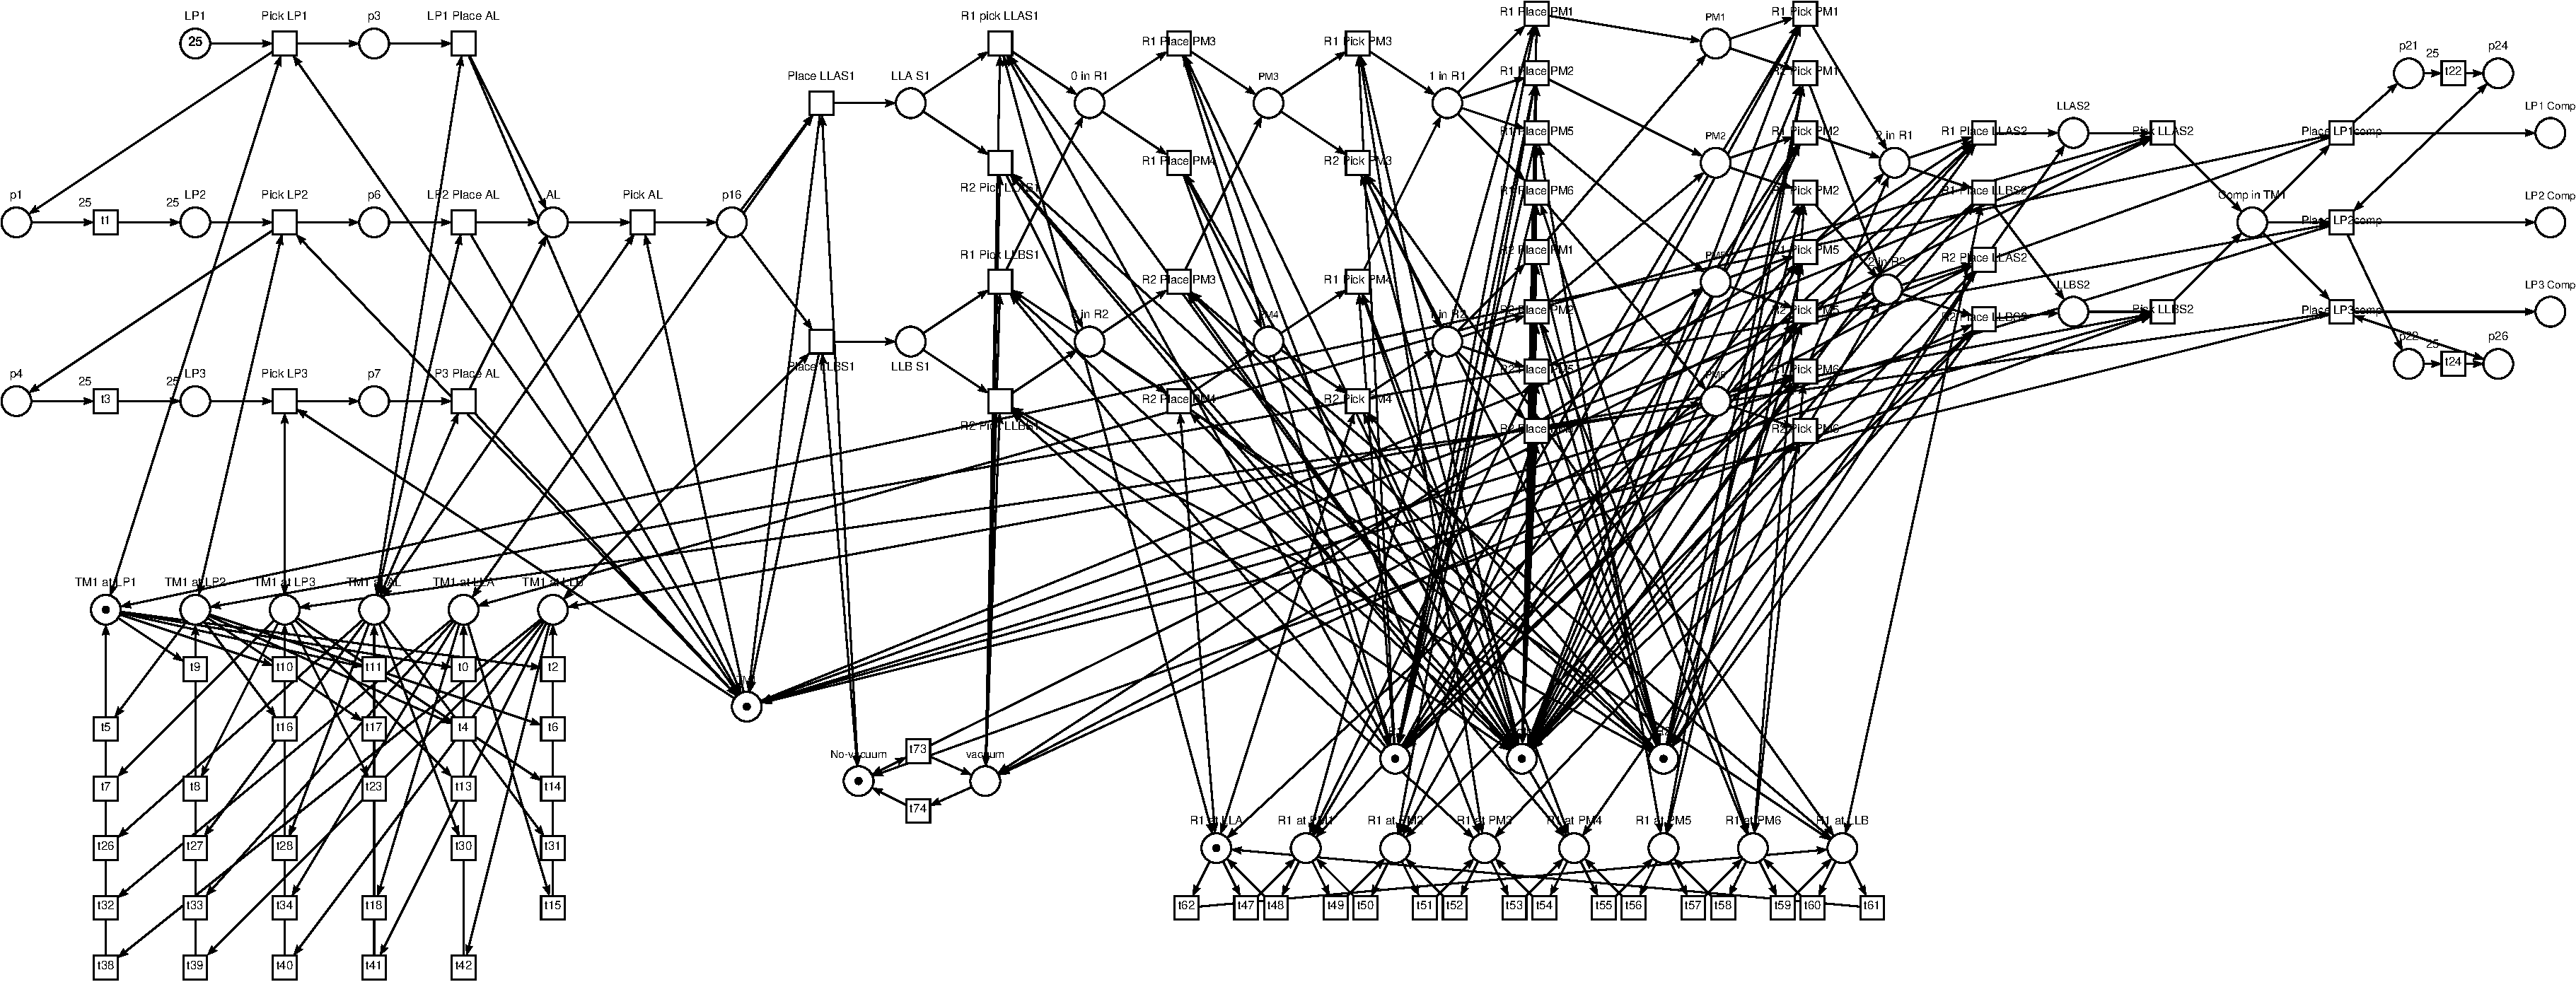
\includegraphics[width=\linewidth]{figures/国赛问题一完全.pdf}\\
	\caption{实际晶圆制造系统}
\end{figure}

本文第四章将使用蚁群算法对此模型进行调度。
\section{本章小结}
本章在上一章的基础上,将库所时间网和变迁时间网结合起来,提出了一种新的时间网子类:库所变迁时间网(TTPPN);
设计了一套TTPPN发射变迁的流程,供下一章的调度算法使用;
设计了一种计算各种Petri网模型的程序架构;
最后使用TTPPN对一个实际的晶圆制造系统进行建模。
% \chapter{基于库所变迁时延网的蚁群算法研究}
第二章介绍了一系列的时间Petri网,第三章提出了一种称为TTPPN的时间网子类,
并基于TTPPN对一个实际的半导体晶圆生产系统进行了建模。

本章将基于上章建立的TTPPN模型,使用算法计算出一条变迁序列。
TTPPN发射此变迁序列,会到达一个规定好的终止标识。
在实际的半导体晶圆生产系统中,最开始,晶圆会堆放在一个腔体中。
随着加工过程的运行,晶圆会被带离初始的腔体,经过一系列的环节,最终被放入到另一个腔体中。
在TTPPN中,这些腔体可被建模为库所。
因此算法的任务即为寻找一条能将一个库所中所有托肯转移到另一个库所中的变迁序列。

另外,按上一章的变迁发射逻辑,每个变迁发射都会有一个具体的时刻,将此时刻作为一个属性存入TTPPN的标识中,称为全局时刻。
TTPPN发射变迁序列生成的最终标识的全局时刻即为此系统完成晶圆加工的总耗时,称为完工时间。
实际情况下,需要完工时间越短越好。这个值将用来衡量算法的解质量。
算法从开始到找到终止标识所消耗的时间称为程序运行时间。这个值将用来衡量算法的速度。
对于启发式算法、群体智能算法来说,时间复杂度的分析十分困难。另外程序运行时间还会受操作系统进程调度策略的影响,未必能如实反映算法速度。
因此本章将记录Petri网的发射次数,用以作为分析算法速度的补充数据。
当Petri网的库所、变迁数确定时,发射变迁产生新标识的时间开销也是确定的。
而对于蚁群算法,其大部分时间开销是发射变迁带来的,因此用发射次数来表征算法的速度。
\section{基于TTPPN的基本蚁群算法}
蚁群算法(Ant Clony Optimization, ACO)是一种群智能算法,
它是由一群无智能或有轻微智能的个体(Agent)通过相互协作而表现出智能行为,
从而为求解复杂问题提供了一个新的可能性。
蚁群算法最早是由意大利学者Colorni A., Dorigo M. 等于1991年提出。
算法运行时蚂蚁会以更高的概率选择信息素浓度高的路,
而蚂蚁会为长度短的路留下更多的信息素。
因此选路机制与信息素添加机制构成了一个正反馈的逻辑,
随着程序的持续运行,正反馈会将解往更优的方向引导\cite{blum2003metaheuristics}\cite{li2015survey}\cite{colorni1992distributed}\cite{kennedy1995particle}\cite{dorigo2004ant}。

TTPPN为时间网,其托肯和变迁上均有时钟,
如果要完整的表示TTPPN,需要记录每一个托肯和变迁上的时钟。
即便两标识中所有库所中的托肯数都相同,但只要托肯上的时钟计时不同,
依然要视为不同的标识。
因此TTPPN与其不加时间的网相比,可达图会异常庞大。

但是在蚁群算法中,即便不存储TTPPN的完整信息,依然可以保证上述正反馈逻辑。
当区分标识仅考虑标识的库所向量时,可达图便可看作是一个边上权值可变的有向图。
\begin{figure}[H]
	\centering
	% Requires \usepackage{graphicx}
	\includegraphics[scale=0.7,angle=0]{figures/可变权值图.pdf}\\
	\caption{可变权值图}
\end{figure}
边上权值会受到初始标识到此标识路径的影响。
选路机制与信息素添加机制构成的正反馈逻辑并不会被破坏,
因此即便不区分时钟计时不同的标识,依然可以使用蚁群算法。

基于TTPPN的基本蚁群算法可分为三个阶段:蚂蚁循迹阶段、信息素稀释阶段和信息素添加阶段。

\begin{algorithm}[H]
    \caption{基于TTPPN的基本蚁群算法}
    \hspace*{0.02in} {\bf 输入:} 
    变迁库所时间网$TTPPN$,变迁库所时间网的初始标识$initMarking$,蚂蚁只数$antCount$,算法迭代轮数$round$\\
    \hspace*{0.02in} {\bf 输出:}
	变迁序列$trans$
    \begin{algorithmic}[1]
		\For {$i \leftarrow 1, round$}
			\State $Ants \leftarrow$初始化$antCount$只蚂蚁放入蚂蚁集合
			\State $RG \leftarrow$初始化一个空的可达图
			\State $antsTravel(Ants,RG,TTPPN,initMarking)$ //蚂蚁循迹阶段
			\State $dilute(RG)$ //信息素稀释阶段
			\State $putPheromone(RG,Ants)$ //信息素添加阶段
		\EndFor
		\State 返回找到的最优变迁序列$trans$
    \end{algorithmic}
\end{algorithm}

蚂蚁循迹阶段是算法的主要流程,本阶段中每只蚂蚁都会独立地在可达图中进行搜索。

\begin{algorithm}[H]
	\caption{蚂蚁循迹阶段}
	\label{alg4-2}
	\begin{algorithmic}
		\Procedure {antsTravel}{$Ants$,$RG$,$TTPPN$,$initMarking$}
		\ForAll{$ant \in Ants$} //$Ants$为蚂蚁的集合
			\State $antTravel(ant,RG,TTPPN,initMarking)$ //单只蚂蚁循迹
		\EndFor
		\EndProcedure
	\end{algorithmic}
\end{algorithm}

每只蚂蚁都有一个禁忌表,蚂蚁每次会选择发射一个变迁,并把发射变迁生成的标识存入此禁忌表中,之后的搜索过程会禁止发射到禁忌表中已经有的标识,
避免蚂蚁走重复的路。
此蚂蚁共有两种结局:1、蚂蚁走到终点标识;2、蚂蚁无路可走。

\begin{algorithm}[H]
	\caption{单只蚂蚁循迹}
	\label{alg4-3}
	\begin{algorithmic}
		\Procedure {antTravel}{$ant$,$RG$}
		\State $tabu \leftarrow$ 初始化蚁群禁忌表
		\State $log \leftarrow$ 初始化蚂蚁日志
		\While {蚂蚁未到达终点并且未走到死路} 
			\State $next(ant,RG,TTPPN,initMarking,tabu,log)$ //为蚂蚁选择变迁并发射的逻辑
		\EndWhile
		\EndProcedure
	\end{algorithmic}
\end{algorithm}

蚂蚁无路可走既可能是因为蚂蚁走上了死锁标识,没有使能变迁可以发射,也可能是此标识的所有使能变迁发射后的标识均在禁忌表中出现过了。
蚂蚁会一直搜索下去直到走到终点,蚂蚁在搜索过程中会记录发射的变迁序列,用以更新可达图上的信息素和输出最后的解。
因为每只蚂蚁的搜索过程相互独立,所以每只蚂蚁搜索过程可由独立的线程并发执行,以提升效率。
蚁群算法的可达图是不带有时间信息的,仅由标识与标识通过使能变迁连接,标识为图的节点,变迁为图的有向弧。
变迁上有一个权值,称为信息素浓度,蚂蚁会根据信息素浓度,并综合考虑到禁忌表,随机选择一个使能变迁发射。
如果蚂蚁到达的标识之前未被添加进可达图,则默认这个标识的所有使能变迁上的信息素浓度是相同的。

\begin{algorithm}[H]
	\caption{蚂蚁选择变迁并发射的逻辑}
	\label{alg4-4}
	\begin{algorithmic}
		\Procedure {next}{$Ants$,$RG$,$TTPPN$,$initMarking$,$ant$,$RG$}
		\State $t=chose(RG,initMarking)$
		\State $initMarking=lanuch(TTPPN,initMarking,t)$
		\State 将当前标识添加进禁忌表$tabu$中
		\State 将发射的变迁$t$记录在蚂蚁日志$log$中
		\EndProcedure
	\end{algorithmic}
\end{algorithm}

\textbf{定义4.1}\textbf{:}
记$P_{Mt}$为可达图中标识$M$的变迁$t$上的信息素浓度,$P_{Mt}\in \mathbb{R}$。
处于标识$M$的蚂蚁选择发射变迁$t$的概率为
$
	\frac{P_{Mt}}{\sum_{i \in T} P_{Mi} }
$。
蚂蚁随机选择变迁发射的算法为轮盘赌算法。
如果有n个待选择的元素,此算法会生成n个彼此相邻的区间,区间的长度与此元素被选择的概率成正比。
算法会随机生成一个大于0,小于区间长度的数值。
这个数值落在哪个区间内,算法就会选择哪个数。

\begin{algorithm}[H]
	\caption{蚁群算法中的轮盘赌算法}
	\label{alg4-5}
	\begin{algorithmic}
		\Procedure {chose}{$RG$,$initMarking$}
		\State $total \leftarrow 0$
		\State $probability \leftarrow $ 用于存储变迁和变迁上信息素浓度的键值对集合
		\State 
		\ForAll{$t \in T$}
			\If{$t^{-} \le m$}
				\State $next \leftarrow lanuch(TTPPN,initMarking,t)$
				\If{$next \in tabu$}
					\State continue
				\EndIf
				\State $value \leftarrow$ 变迁$t$上的信息素浓度
				\State $total=total+value$
				\State $put(probability,t,value)$ //$put(probability,t,value)$指在键值对集合probability中添加键值对$(t,value)$
			\EndIf
		\EndFor
		\State $random \leftarrow $随机生成一个大于0,小于$total$的数
		\State $total=0$
		\ForAll{$t \in keys(probability)$} //$keys(probability)$表示键值对集合$probability$中键的集合
			\State $value \leftarrow get(probability,t)$ //$get(probability,t)$表示从键值对集合$probability$中取键$t$的值
			\State $total=total+value$
			\If{$total \ge random$}
				\State return true
			\EndIf
		\EndFor
		\EndProcedure
	\end{algorithmic}
\end{algorithm}

蚂蚁会根据可达图变迁上的信息素浓度的大小,随机选择一个变迁发射,并在走到终点后,为可达图增加信息素。
随着蚁群算法不断运行下去,可达图中的信息素浓度会越来越高,导致之后蚂蚁添加的信息素占总信息素浓度的比重越来越低。
在这种情况下,后期蚂蚁对解的影响将会减少。
而前期可达图中信息素尚少,蚂蚁循迹几乎是随机的,所以后期的蚂蚁比前期的蚂蚁更为重要。
因此应该加入信息素稀释机制。

\textbf{定义4.2}\textbf{:}
记$\alpha $为信息素稀释率,$\alpha \in \mathbb{R}$,$P_{Mt}^{i}$为蚁群算法第$i$轮中$P_{Mt}$的值。
记$A_{Mt}^{ji}$为第$j$只蚂蚁第$i$轮要在标识$m$上添加的信息素浓度。
$P_{Mt}^{i+1}=\alpha P_{Mt}^{i}+A_{Mt}^{ji}$

每轮可达图上的信息素都会按比例被稀释掉。
\begin{algorithm}[H]
	\caption{信息素稀释阶段}
	\label{alg4-6}
	\begin{algorithmic}
		\Procedure {dilute}{$RG$}
			\ForAll{$M \in RG$}
				\ForAll{$t \in T$}
					\State $P_{Mt}=\alpha P_{Mt}$
				\EndFor
			\EndFor
		\EndProcedure
	\end{algorithmic}
\end{algorithm}

蚁群在循迹过程中,会将到达终点标识的变迁标识序列保存起来,称为蚂蚁日志(log),并在添加信息素阶段根据蚂蚁日志,更新信息素。
如果蚂蚁日志中的标识已经在可达图中存在,则直接更新其上的信息素。
如果此标识之前从未被放入可达图,则在此时放入可达图。
因此蚁群算法的可达图是随着算法运行,逐渐扩展出来的,并不需要一开始就提供。
信息素的添加量要和路径长度成反比,在我们时间网的场景下,蚂蚁日志中的变迁标识序列中最后一个标识记录的时刻是完成调度的总耗时。
因此信息素的添加量应与这一时刻成反比。

\textbf{定义4.3}\textbf{:}
记$T_{ji}$为第$j$只蚂蚁第$i$日志的变迁标识序列中最后一个标识记录的时刻,此蚂蚁要在标识$m$上添加的信息素浓度$A_{Mt}^{ji}=\frac{C}{T_{ji}} $。

\begin{algorithm}[H]
	\caption{信息素添加阶段}
	\label{alg4-7}
	\begin{algorithmic}
		\Procedure {putPheromone}{$RG$,$Ants$}
			\ForAll{$ant \in Ants$}
				\ForAll{$M \in Markings(log)$} \\$Markings(log)$为蚂蚁日志log中的标识序列
					\If{$M \in RG$}
						\State $P_{Mt}=A_{Mt}$
					\Else
						\State 将$M$放入$RG$中
						\State $value \leftarrow 默认值$
						\State $P_{Mt}=value$
					\EndIf
				\EndFor
			\EndFor
		\EndProcedure
	\end{algorithmic}
\end{algorithm}
上述流程如果以单只蚂蚁为粒度,进行并发计算,无线程安全问题容易解决。
因为每只蚂蚁所需要的资源仅有两种:可达图、蚂蚁日志。
其中日志为每只蚂蚁私有资源,其他蚂蚁无权操作,因此无线程冲突。
而蚂蚁对于可达图有两种操作:读、写。
写操作只发生在稀释和更新信息素阶段。
而读操作发生在蚂蚁循迹阶段。
读写操作是分离的。
因此读操作不存在线程冲突。

对于写操作,有线程安全问题,因此需要加锁,并发度不如其他流程。
但通过合理选择可达图的数据结构,可以尽可能提升并发度。

\section{蚁群可达图使用的数据结构}
蚂蚁在循迹阶段,需从可达图上得出当前标识上各个使能变迁的信息素浓度。
因此蚂蚁对可达图有查询操作。

在信息素浓度稀释阶段,可达图上各个变迁的信息素浓度需按比例稀释。
因此可达图需支持修改数据的操作。

在添加信息素阶段,蚂蚁有可能探索到从未被发现的标识。
需要将这个标识的信息加入可达图中。
因此蚂蚁对可达图有添加信息的操作。

随着算法的一轮轮迭代,某些标识上的使能变迁的信息素已经被稀释到很低了。
蚂蚁走上此标识的概率极小,即便走上了,其使能变迁上信息素浓度也近乎均匀。
因此应该从可达图中删除这类标识,以节约内存。

基于以上的分析,蚁群算法的可达图需支持增、删、改、查四种操作。
所以应该选择增、删、改、查复杂度均为$O(1)$的哈希表作为数据结构实现。

可达图在算法流程中需写入数据,此操作有线程安全问题,因此需要对其加锁。
一下两种为哈希表的常规加锁方式。
\subsection{对操作方法加锁}
当算法中有线程要对可达图进行写入操作时,
需尝试取得写入操作的锁,
并在写入完成后释放锁。
锁的数量只有一个。
对于取得锁和释放锁的逻辑,均调用操作系统自带的原语以保证原子性。
如果某流程具有原子性,则此流程只有两种状态:未开始状态、已完成状态。
因此可以使用CAS原语实现加锁。
CAS的功能是将某地址的值与给定值比较并交换,并根据比较结果返回特定值。
CAS方法具有原子性,利用CAS方法的特点可以设计互斥锁。
互斥锁实现方法如下:

1、判断CAS操作是否成功,如果不是则重复此步;

2、执行写可达图的操作;

3、使用CAS将特定地址的值置回初值。


使用此逻辑,保证了不可能有两个线程同时修改可达图,从根本上解决了线程安全问题。
但是这种加锁逻辑,过于粗糙,大大降低了并发度。

使用CAS锁,如果某线程未取得锁,它会一直尝试取得锁。
可以使用信号量机制,直接让处理机暂停执行此线程,从而执行其他线程,来提高效率。
\subsection{对数据加锁}
即便是对可达图进行修改,如果修改的不是同一个标识的数据,也是不会有线程安全问题的。
而同时对同一个标识进行写操作,完全是小概率事件。
所以对具体标识进行加锁是更为高效的选择。

基于哈希表的底层原理,实际上是对哈希表内部数组的各个地址进行加锁,锁的数量最多为内部数组长度。
当写操作需要处理某地址的数据,先尝试取得此地址上的锁,并在写入完成后释放锁。

锁的数量增加会带来额外的内存开销。
如果需减少这部分的内存开销可以将锁加在地址的区间上,以减少锁的数量。
\section{备份可达图提高算法并发度}
本算法分为三个阶段:蚂蚁循迹阶段、信息素稀释阶段、信息素添加阶段。
原算法中三阶段是串行的。
蚂蚁需要先循迹,得到解后才能添加信息素,因此第一阶段和第三阶段存在依赖关系,必然是串行的。
然而第二阶段和一、三阶段的依赖关系并不明确。
理论上第二阶段和第三阶段可看作是一个大阶段,
即更新信息素阶段。
而第一阶段和第三阶段本质上并没有依赖关系,
只因为第一阶段蚂蚁循迹需要读可达图,第二阶段可达图稀释需要写可达图,
因此为保证线程安全,将其分为两个阶段。

如果将可达图备份一份,这两个阶段是可以并发执行的。

现将可达图分为两份,主可达图($RG$)与副可达图($RGCopy$)。
这两份可达图互为副本,在之后蚁群算法一轮轮迭代中会交替充当主可达图供蚁群使用。

在蚂蚁循迹阶段另外加入一个线程,专门用于完成可达图备份与稀释。

主可达图因为上一轮被修改了信息,这部分信息未被加入副可达图中,
副可达图也需要同步这部分修改。

修改的内容分为三部分:对原标识的信息素更新、添加新标识、删除信息素浓度过低的标识。
因此需遍历原可达图,并基于此修改副可达图的信息。
再遍历副可达图,删除原可达图中不存在的标识。

完成蚂蚁循迹流程后,交换原副可达图。

\begin{algorithm}[H]
	\caption{备份可达图}
	\label{alg4-9}
	\begin{algorithmic}
		\Procedure {copy}{$RG$,$RGCopy$}
			\ForAll{$m\in RG$}
				\If{$m \in RGCopy$}
					\State 同步$m$上的信息素浓度
				\Else
					\State 将$m$添加入$RGCopy$中
				\EndIf
			\EndFor
				\ForAll{$m \notin  RGCopy$}
				\If{$m \in RG$}
					\State 从$RGCopy$中删除$m$
				\EndIf
			\EndFor
		\EndProcedure
	\end{algorithmic}
\end{algorithm}

\section{蚁群求解实际问题}
本节将使用蚁群算法求解第四章对实际晶圆生成系统建立的模型。
为衡量蚁群算法解的质量,需要知道模型的最优调度策略。
本节将使用迪杰斯特拉算法求解Petri网模型的最优变迁序列。
\subsection{基于迪杰斯特拉算法求解Petri网最优变迁序列}
迪杰斯特拉算法用于求取图的最短路径。
如果图的节点数为n,此算法可以在$O(nlog(n))$的时间复杂度下得出各节点到起点的最短路径。

基于时间网的背景,设计迪杰斯特拉算法。

\subsubsection{存放将要扩展的标识的集合}
设计一个集合,此集合专门用于存放接下来将要扩展的标识,命名为$OPEN$集合。
Petri网的可达图是随算法运行动态添加进内存中的,所以$OPEN$中一开始只有初始标识,
随着程序的运行,如果遇到有扩展价值的标识,此标识会被放入$OPEN$中。

$OPEN$会被取出标识进行扩展,也会被放入标识。
但基于迪杰斯特拉算法的机制,取出的标识应该是集合中离原点最近的标识,
也就是全局时间最短的标识。

如果遍历这个集合寻找全局时间最短的标识,当集合大小为$n$时,其时间复杂度为$O(n)$。
但是如果使用小根堆去实现,其时间复杂度为$O(log(n))$。
因此本算法将使用小根堆作为此集合的实现。

\subsubsection{已经扩展的标识的集合}
此集合专门用于存放已经扩展的标识,命名为$CLOSE$集合。
当一个标识从$OPEN$取出,并且它的所有变迁均被处理过,就会放入此集合中。
因为每次处理的标识都是$OPEN$中全局时间最短的标识,
所以当此标识进入$CLOSE$中,如果之后再扩展到它,如果时间网可达图路径上的时间间隔是确定的,其全局时间必然更长。
所以当标识已经在$CLOSE$中了,是没有扩展的意义的。

但实际上时间网可达图路径上的权值是可变的,所以$CLOSE$表中存储的为键值对,键为标识,值为目前到达此标识的最短时间。
此后判断标识是否值得扩展,应该判断到达此标识的全局时间是否比$CLOSE$表中记录的最短时间短,
如果此时间确实更短,才去扩展此标识。

$CLOSE$涉及到两种操作:将已完成扩展的标识存入此集合中、查询标识是否在此集合中。
因此本算法选取哈希表作为此集合的数据结构实现。哈希表存与查的时间复杂度均为$O(1)$。
使用哈希表实现的$CLOSE$其底层是一个固定长度的数组。
标识需要得到$CLOSE$底层数组的一个元素索引,才能进入$CLOSE$表。
进入$CLOSE$表的标识会被存放在特定索引上。
此索引是根据哈希值得出的,哈希值是使用哈希函数得出的,哈希函数的输入是标识向量。
对于哈希值相同的标识,本$CLOSE$表会将其统一存放在一棵红黑树中。
如果红黑树的节点数为$n$,其增删改查的时间复杂度是$log(n)$。

\subsection{算法流程}
迪杰斯特拉算法每次会从$CLOSE$中取一个全局时间最短的标识$curr$,如果此标识就是终点标识,则找到终点。
如果$CLOSE$集合取空都未找到终点,则说明终点不可达。
对$curr$的所有使能变迁均发射一次,如果发射产生的新标识$next$已经在$OPEN$中存在,并且其全局时间更短,则将其取出,更新其全局时间后再放入。
在$OPEN$中查询标识的时间复杂度为$O(log(n))$,往其放入标识的时间复杂度为$O(log(n))$。
如果$next$的全局时间已经高于$CLOSE$中对于标识处记录的最短时间,则没有必要扩展此标识,如果不存在,之前查找时也没在$OPEN$中找到就将此标识放入$OPEN$中。
当$curr$的所有使能变迁均处理完成,将其放入$CLOSE$中。

迪杰斯特拉算法流程如下所示:

\begin{algorithm}[H]
    \caption{基于时间网的迪杰斯特拉算法}
    \hspace*{0.02in} {\bf 输入:} 
    变迁库所时间网$TTPPN$,变迁库所时间网的初始标识$initMarking$,终点标识$endMarking$\\
    \hspace*{0.02in} {\bf 输出:}
	变迁序列$trans$
    \begin{algorithmic}[1]
		\For {$i \leftarrow 1, round$}
			\State 往$OPEN$放入初始标识$initMarking$
			\While{$OPEN$不为空}
				\State $curr \leftarrow$从$OPEN$中取出全局时间最小的标识
				\ForAll{$t\in curr$的使能变迁}
					\State $next \leftarrow launch(TTPPN,curr,t)$
					\If{$next$在$OPEN$中且全局时间更短}
						\State 更新$OPEN$中$next$的全局时间
					\EndIf
					\If{$next$值得扩展}
					\State 将$next$放入$OPEN$
					\EndIf
				\EndFor
				\State 将$curr$放入$CLOSE$中
			\EndWhile
		\EndFor
		\State 返回找到的最优变迁序列$trans$
    \end{algorithmic}
\end{algorithm}

\subsection{实验和结果分析}
在处理器为i5-1130G7,最大内存为8GB的设备上,排除文件读入、结果输出的耗时,仅在调用算法前后记录系统时间戳,
分别使用迪杰斯特拉算法和蚁群算法求解第五章建立的晶圆制造系统的模型。

\subsubsection{迪杰斯特拉算法的实验结果分析}
以下是使用6GB内存,迪杰斯特拉算法的结果。

变迁序列为:$t_{1}$->$t_{7}$->$t_{1}$->$t_{2}$->$t_{1}$->$t_{17}$->$t_{3}$->$t_{7}$->$t_{16}$->$t_{1}$->$t_{23}$->$t_{2}$->$t_{1}$->$t_{17}$->
$t_{27}$->$t_{7}$->$t_{16}$->	$t_{1}$->$t_{2}$->$t_{1}$->$t_{4}$->$t_{14}$->$t_{24}$->$t_{12}$->$t_{22}$->$t_{1}$->
$t_{13}$->$t_{29}$->$t_{11}$->$t_{22}$->$t_{1}$->$t_{14}$->$t_{12}$->$t_{22}$->$t_{20}$->$t_{18}$->$t_{1}$->$t_{4}$->$t_{14}$->
$t_{24}$->$t_{12}$->$t_{22}$->$t_{20}$->$t_{18}$->$t_{13}$->$t_{1}$->$t_{29}$->$t_{11}$->$t_{22}$->$t_{20}$->$t_{18}$->$t_{14}$->
$t_{1}$->$t_{12}$->$t_{22}$->$t_{20}$->$t_{18}$->$t_{1}$->$t_{4}$->$t_{14}$->$t_{24}$->$t_{12}$->$t_{22}$->$t_{20}$->$t_{18}$->
$t_{13}$->$t_{20}$->$t_{18}$->$t_{8}$->$t_{29}$->$t_{22}$->$t_{14}$->$t_{20}$->$t_{18}$->$t_{9}$->$t_{22}$->$t_{20}$->$t_{18}$->
$t_{20}$->$t_{18}$->$t_{4}$->$t_{10}$->$t_{9}$->$t_{24}$->$t_{22}$->$t_{6}$->$t_{8}$->$t_{22}$->$t_{28}$->$t_{10}$->$t_{20}$->
$t_{18}$->$t_{9}$->$t_{22}$->$t_{20}$->$t_{18}$->$t_{20}$->$t_{18}$->$t_{4}$->$t_{10}$->$t_{9}$->$t_{22}$->$t_{20}$->$t_{18}$

完工时间为:1600.8s

程序运行时间为:8.972s

迪杰斯特拉算法每次都会选取离起点最近的节点进行扩展,因此扩展过程为一层层推进,其扩展过的可达标识数与可达图成比例。
本算法在使用变迁发射方法$launch$时会使用到标识的时钟信息,
而时间网的标识数巨大,为节约内存开销,本算法仅将标识向量存入$CLOSE$中。
因此在扩展过程中会产生大量的垃圾信息,需要被垃圾回收。
内存大小影响垃圾回收的次数,内存越大,垃圾回收次数越少。

分别测试从1GB内存到6GB内存迪杰斯特拉算法的程序运行时间。

\begin{table}[H]
	\centering
	\caption{内存与程序运行时间关系}
	\resizebox{!}{!}{
		\begin{tabular}{l|lllllllll}
			\toprule
			内存(GB) & 1 & 2 & 3 & 4 & 5 & 6 \\ \hline
			程序运行时间(s) & 12.695 & 10.930 & 9.031 & 8.752 & 8.803 & 8.972 \\
			\bottomrule
		\end{tabular}
	}
\end{table}

\begin{figure}[H]
	\centering
	% Requires \usepackage{graphicx}
	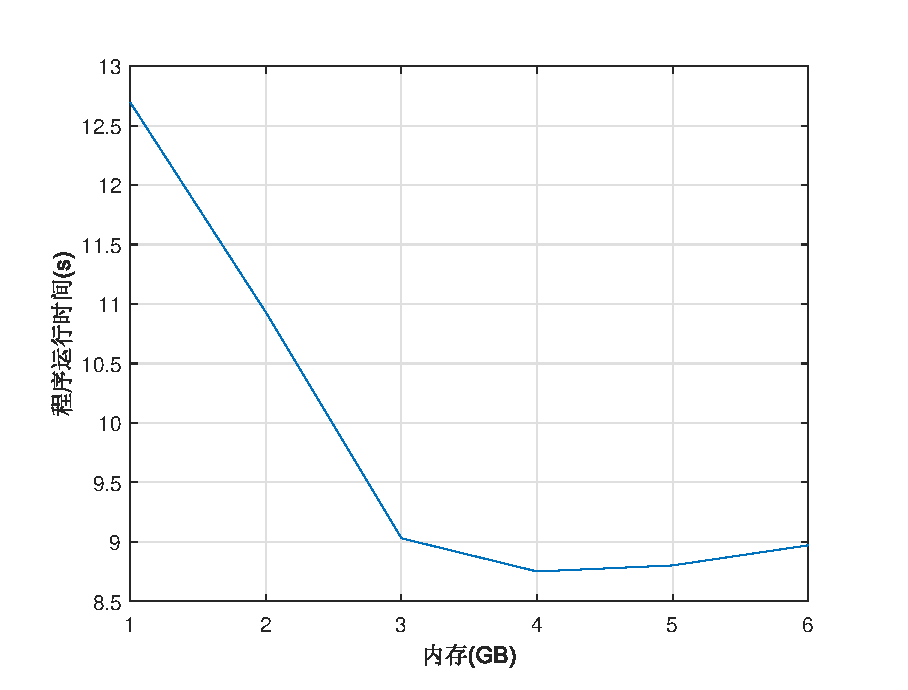
\includegraphics[scale=1.00,angle=0]{figures/mem_t.eps}\\
	\caption{迪杰斯特拉算法内存与程序运行时间关系}
\end{figure}

如上图所示,随着内存的增加,程序运行时间有下降的趋势,当内存增加到3GB时,程序运行时间稳定在9s左右。

\subsubsection{蚁群算法的实验结果分析}
以下是使用6GB内存,蚁群算法100只蚂蚁迭代100轮的结果。

变迁序列:$t_{1}$->$t_{2}$->$t_{1}$->$t_{7}$->$t_{17}$->$t_{3}$->$t_{16}$->$t_{23}$->$t_{1}$->$t_{2}$->$t_{1}$->$t_{4}$->$t_{13}$->$t_{24}$->$t_{7}$->$t_{14}$->$t_{3}$->$t_{4}$->$t_{9}$->$t_{10}$->$t_{24}$->$t_{22}$->$t_{1}$->$t_{11}$->$t_{13}$->$t_{23}$->$t_{21}$->$t_{19}$->$t_{12}$->$t_{21}$->$t_{18}$->$t_{17}$->$t_{20}$->$t_{18}$->$t_{1}$->$t_{27}$->$t_{24}$->$t_{10}$->$t_{28}$->$t_{12}$->$t_{14}$->$t_{23}$->$t_{22}$->$t_{8}$->$t_{21}$->$t_{24}$->$t_{6}$->$t_{19}$->$t_{12}$->$t_{22}$->$t_{17}$->$t_{8}$->$t_{27}$->$t_{22}$->$t_{1}$->$t_{7}$->$t_{1}$->$t_{17}$->$t_{7}$->$t_{20}$->$t_{18}$->$t_{23}$->$t_{1}$->$t_{2}$->$t_{1}$->$t_{17}$->$t_{7}$->$t_{20}$->$t_{19}$->$t_{3}$->$t_{28}$->$t_{14}$->$t_{27}$->$t_{12}$->$t_{21}$->$t_{16}$->$t_{18}$->$t_{24}$->$t_{14}$->$t_{4}$->$t_{9}$->$t_{21}$->$t_{18}$->$t_{6}$->$t_{28}$->$t_{8}$->$t_{6}$->$t_{24}$->$t_{10}$->$t_{22}$->$t_{4}$->$t_{9}$->$t_{10}$->$t_{21}$->$t_{18}$->$t_{9}$->$t_{22}$->$t_{20}$->$t_{18}$->$t_{8}$->$t_{21}$->$t_{18}$->$t_{20}$->$t_{18}$->$t_{20}$->$t_{18}$

完工时间:2554.7s

程序运行时间:23.374s

此结果无论是完工时间还是程序运行时间,均要长于迪杰斯特拉算法的解。

导致此结果的可能原因有3个:算法不能收敛、算法收敛到较差解、算法收敛慢。

基于以上的分析,设计实验。
依次提高迭代轮数,观察完工时间,如果随迭代轮数增加,完工时间分布随机,则说明算法未收敛。
如果随迭代轮数增加,完工时间区域稳定值,并且稳定值接近迪杰斯特拉算法的解,说明算法收敛慢,如果稳定值显著高于迪杰斯特拉的解,
说明算法收敛到较差解。

另外,在计算机CPU有限的情况下,提高蚂蚁只数会时程序频繁进行线程切换,增大程序运行时间。
使用需要探寻蚂蚁只数与算法效率的关系。

将迭代轮数从10轮每次递增10轮直到100轮,统计完工时间,观察蚁群算法是否有收敛趋势。

\begin{table}[H]
	\centering
	\caption{蚁群算法迭代轮数与完工时间的关系}
	\resizebox{\linewidth}{!}{
		\begin{tabular}{l|lllllllllllll}
			\toprule
				轮数 & 10 & 20 & 30 & 40 & 50 & 60 & 70 & 80 & 90 & 100 \\ 
				\hline
				完工时间(s) & 2554.7 & 2254.1 & 1956.1 & 1921.7 & 2223.8 & 2494.7 & 2513.5 & 2487.9 & 2393.8 & 2554.7 \\
				\bottomrule
			\end{tabular}
	}
\end{table}

如图所示,蚁群算法在本场景下并没有收敛,迭代轮数在30轮之前,完工时间有下降趋势,但随着轮数的增加,完工时间也增加,最终有稳定在2500.0s的趋势。

从这个结果可以看出,此蚁群算法收敛到一个较差的解上,而且并不是收敛到局部最优解,因为随着迭代轮数增加,算法曾到达了较优的解,但依然有向差解接近的趋势。

为证明前30轮确实有下降趋势,而非是偶然现象,将迭代轮数从1轮每次递增10轮直到10轮,统计完工时间。

\begin{table}[H]
	\centering
	\caption{蚁群算法迭代轮数与完工时间的关系(小轮数)}
	\resizebox{\linewidth}{!}{
		\begin{tabular}{l|lllllllllllll}
			\toprule
			轮数 & 1 & 2 & 3 & 4 & 5 & 6 & 7 & 8 & 9 & 10 \\ \hline
			完工时间(s) & 3274.6 & 3136.1 & 3153.8 & 3024.6 & 2952.2 & 2840.0 & 2708.3 & 2630.0 & 2600.5 & 2554.7 \\
			\bottomrule
		\end{tabular}
	}
\end{table}

\begin{figure}[H]
	\centering
	% Requires \usepackage{graphicx}
	\includegraphics[scale=1.00,angle=0]{figures/round_t_small.eps}\\
	\caption{蚁群算法迭代轮数与完工时间关系(1到10轮)}
\end{figure}

如上图所示,低轮数时蚁群算法确实有收敛趋势。

本程序中每只蚂蚁都是一个线程,如果线程数量小于CPU数量,各个线程能并行指向,彼此互不影响。
而如果线程数量高于CPU数量,CPU就需要不断第切换到不同的线程,以实现程序并发地执行。
如果两线程竞争一个CPU,必然会导致其中一个线程等待。
因此随蚂蚁只数增加,程序运行时间会增加。
此外线程切换本身也是有开销的。
所以需要探寻蚁群算法蚂蚁只数对完工时间的影响,得出一个恰当的蚂蚁只数,并以此合理配置CPU数量。

为了观察蚂蚁只数对算法收敛性的影响,固定迭代轮数为10轮,从10只蚂蚁每次递增10只直到100只对此模型进行求解,观察完工时间。

\begin{table}[H]
	\centering
	\caption{蚁群算法蚂蚁只数与完工时间的关系}
	\resizebox{\linewidth}{!}{
		\begin{tabular}{l|lllllllllllll}
			\toprule
				蚂蚁只数 & 10 & 20 & 30 & 40 & 50 & 60 & 70 & 80 & 90 & 100 \\ \hline
				完工时间(s) & 2799.9 & 2404.6 & 3184.9 & 2314.9 & 2637.2 & 2718.6 & 2599.7 & 2596.0 & 2894.7 & 2554.7 \\
			\bottomrule	
		\end{tabular}
	}
\end{table}

\begin{figure}[H]
	\centering
	% Requires \usepackage{graphicx}
	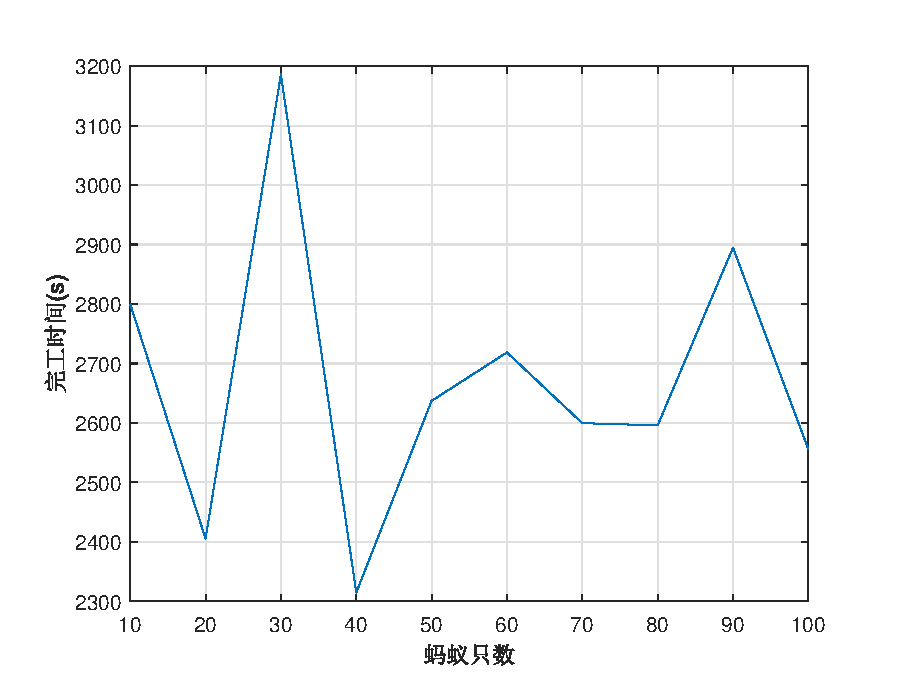
\includegraphics[scale=1.00,angle=0]{figures/count_t.eps}\\
	\caption{蚁群算法迭代轮数与完工时间关系(1到10轮)}
\end{figure}

如上图所示,随着蚂蚁只数的增加,完工时间是随机的,这意味着可能10只蚂蚁以后,蚂蚁只数就对算法收敛性影响不大了。

为表明低蚂蚁只数时,蚂蚁只数对算法收敛是有影响的,固定迭代轮数为10轮,从1只蚂蚁每次递增1只直到10只对此模型进行求解,观察完工时间。

如果蚂蚁只数在增加到一定值后,对解质量影响不大,则应该让蚁群算法运行在CPU数量高于此蚂蚁只数的机器上,
以避免线程切换与等待的开销,提升算法运行效率。

但是如果蚂蚁只数较高,应该选择处理器更多的GPU来运行蚁群算法。
本蚁群算法的可达图是动态扩展的,因此存在大量内存申请与清理的操作,此操作不适合在GPU上使用,
所以本文的代码是为CPU编写的。

\begin{table}[H]
	\centering
	\caption{蚁群算法蚂蚁只数与完工时间的关系(小只数)}
	\resizebox{\linewidth}{!}{
		\begin{tabular}{l|lllllllllllll}
			\toprule
			蚂蚁只数 & 1 & 2 & 3 & 4 & 5 & 6 & 7 & 8 & 9 & 10 \\ \hline
			完工时间(s) & 3640.5 & 3760.5 & 3262.0 & 3362.1 & 3256.0 & 3008.7 & 2651.0 & 2684.5 & 2752.9 & 2799.9 \\
			\bottomrule	
		\end{tabular}
	}
\end{table}

\begin{figure}[H]
	\centering
	% Requires \usepackage{graphicx}
	\includegraphics[scale=1.00,angle=0]{figures/count_t_small.eps}\\
	\caption{蚁群算法迭代轮数与完工时间关系(1到10轮)}
\end{figure}

如上图所示,在蚂蚁数量较少时,蚂蚁只数越大,完工时间越小。

综上,提升蚁群算法蚂蚁只数、和算法迭代次数,在一开始会对算法收敛性有较大贡献。随着蚂蚁只数增加到10只后,再增加蚂蚁只数对算法影响不大。
当迭代轮数增加到30轮以后,蚁群算法的解有恶化的趋势,再继续增加迭代轮数会使算法稳定在一个较差的解。

但是无论如何配置蚂蚁只数和迭代轮数,都无法使解向迪杰斯特拉算法求出的解靠近。下一节将继续分析蚁群算法解的情况,并且尝试了一系列优化方案。
\section{改进的蚁群算法}
基于上一小节的数据进行分析,原始的蚁群算法存在求解特定时间网的变迁序列时存在缺陷。
如果某时间Petri网的最优变迁序列上的使能变迁很少,
而完工时间较差的变迁序列彼此又互相连通,
原始蚁群算法便无法收敛。
其原因为走上最优解的蚂蚁有更高的概率走入死锁标识,失去添加信息素的资格。
而走向较差解的蚂蚁会有更高的概率走向终点标识,并在可达图上留下信息素。
原始蚁群算法的正反馈机制被打破,使算法无法收敛。
为修复这一异常,本文对原始蚁群算法进行了如下改进。
\subsection{超级蚂蚁机制}
如果此蚂蚁的解比目前的最优解还优,则赋予它添加更多信息素的权利,能添加的额外的信
息素和对解优化的贡献相关。
这么做是为了削弱之前非最优解的蚂蚁对流程的影响。当某蚂蚁运气好,得出的解远好于目
前的解,便可迅速提升这个解上的信息素,从而将误入歧途的蚂蚁重新引入正轨。

\textbf{定义4.5}\textbf{:}
记$MinTime$为蚁群算法运行时,当前得到的最短完工时间。
$CurrTime$为当前蚂蚁完成循迹后得出的完工时间。
$\beta$为此蚂蚁添加信息素的增益。
\begin{equation}
	\beta=\left\{
		\begin{aligned}
			1 \quad MinTime-CurrTime \leqslant 0\\
			MinTime-CurrTime \quad MinTime-CurrTime > 0\\
		\end{aligned}
		\right.
		\nonumber 
\end{equation}
此蚂蚁添加的信息素应乘上此增益。
因此第$j$只蚂蚁第$i$轮要在标识$m$上添加的信息素浓度$A_{Mt}^{ji}$应修改为
$$
A_{Mt}^{ji}=\beta A_{Mt}^{ji}
$$
当此蚂蚁循迹得出的解好于目前找到的最优解,它添加的信息素会被增益$\beta$放大。
当得出的解的完工时间越短,增益越大。
蚁群算法出现局部收敛时,
使用此机制,蚂蚁只要以小概率探索到了局部以外的更优解,
此解便会被添加大量信息素,
引导其他蚂蚁探索新解,
跳出局部收敛。

此蚂蚁需将找到的解更新为新的最优解。
因此在每只蚂蚁的添加信息素逻辑中需添加一段更新最优解流程。
\begin{algorithm}[H]
	\caption{更新最优解}
	\label{alg4-10}
	\begin{algorithmic}
		\Procedure {renNewMinTime}{}
			\If{$\beta>1$}
			\State $MinTime=CurrTime$
			\EndIf
		\EndProcedure
	\end{algorithmic}
\end{algorithm}

此流程中需修改$MinTime$这一全局变量。
而添加信息素逻辑是并发执行的,因此此处$MinTime$有可能同时被多个线程写入。
但因为此处即便有线程安全问题,也不影响算法执行,因此为提高并发度,不进行加锁。
\subsection{贪心选取初始信息素}
原算法蚂蚁遇到从未走过的地点(没有一只蚂蚁去过的地点),会以平均的概率选取下一步。
如果蚂蚁所在标识的各使能变迁是等价的,并不知道哪个变迁更优,蚂蚁在首次经过此标识时确实应该以平均的概率选择一条变迁。
但结合实际背景,这些变迁并不等价。
加工腔中的晶圆如果加工完毕,应该尽早取走。
基于此特点,
现将蚂蚁初次选路的策略修改为以更大的概率选择近的路。

将原算法中遇到新标识时构建新信息素对象的逻辑修改为以下逻辑。
\begin{algorithm}[H]
	\caption{贪心选取初始信息素}
	\label{alg4-11}
	\begin{algorithmic}
		\Procedure {greedyInitPheromone}{}
			\ForAll{$t\in T$}
				\If{$t^{-} \le m$}
					\State $nextMarking \leftarrow lanuch(currMarking,t)$
					\State 将变迁$t$上的信息素浓度设置为$time(nextMarking)-time(currMarking)$
					\\$time(marking)$为取得标识$marking$全局时间的方法
				\EndIf
			\EndFor
		\EndProcedure
	\end{algorithmic}
\end{algorithm}
对于此标识的所有使能变迁,均发射一次得出此标识的后继标识。
按这些后继标识的全局时间对这些变迁分配初始信息素。
时间越短初始信息素浓度越高。

这是一种贪心的思想。
发射使后继标识全局时间最短的变迁,意味着寻求单步最优的变迁发射。
实际生产系统中单步最优构成的解往往质量不差,因此这种逻辑在某些场景下,效果不错。
但如果模型最优解远离贪心解,此机制探寻新路径时依然会使用贪心的逻辑,会影响算法的收敛效率。
因此下一节将提出一种约束较弱的贪心策略。
\subsection{使用贪心算法预添加信息素}
与上一节使用的思想类似,使用贪心的思想优化算法。
具体逻辑为:
先使用贪心算法求解出一个解,在此解的变迁标识序列上添加一部分信息素。
再使用蚁群算法在此基础上继续求解。

贪心算法会不断地发射使后继标识全局时间最短的变迁,直到找到终点。
因为可达图中存在死锁标识,需为算法加入回溯机制,
遇到死锁标识时,回溯,并发射使后继标识的全局时间次大的变迁。

因此定义一个函数$find(marking)$,
此函数的功能为判断以标识$marking$为初始标识,判断是否能探索到与终点标识连通的路径。
\begin{algorithm}[H]
	\caption{贪心算法}
	\label{alg4-12}
	\begin{algorithmic}
		\Procedure {find}{$marking$}
			\If{$marking$为终点标识}
				\State return true
			\EndIf
			\State 对$marking$的使能变迁按全局时间进行排序,并装入$enableTrans$中
			\ForAll{$t \in enableTrans$}
				\State $nextMarking \leftarrow lanuch(t,currMarking)$
				\If{$nextMarking$被扩展过}
					\State continue
				\EndIf
				\If{$find(nextMarking)$}
					\State return true
				\EndIf
			\EndFor
			\State return false
		\EndProcedure
	\end{algorithmic}
\end{algorithm}
此函数使用递归实现了回溯功能。

在函数运行时一并记录发射的变迁,如果发生回溯,删除回溯的变迁,便得到一条变迁序列。
基于此序列预先为可达图分配信息素。

\subsection{复活蚂蚁}
当蚂蚁走到死锁标识时循迹结束,此时得到的变迁序列并不能到达终点标识,因此无法基于此序列添加信息素。
如果最优解附近存在大量死锁,那么大部分最优解附近的蚂蚁将失去添加信息素的资格,反而使得差解信息素浓度过高。
本节设计了一种机制,可以为使走上死锁的蚂蚁复活。

\textbf{定义4.6}\textbf{:}
记$similarity(s_{1},s_{2})$为标识序列$s_{1},s_{2}$的相似度。\\
$sameMarkingCount(s_{1},s_{2})$为标识序列$s_{1},s_{2}$中相同标识的数量。
$length(s_{1})$为$s_{1}$中标识的数量。\\
计算方法为:
$$
	similarity(s_{1},s_{2})=\frac{sameMarkingCount(s_{1},s_{2})}{length(s_{1})} 
$$

如果此蚂蚁死亡,则将其替换为活蚂蚁中与其相似度最高的蚂蚁。
\subsection{蚁群算法与模拟退火算法结合}
如果蚁群算法真的如预期,应该是会随着迭代次数的增加,收敛到一个最优解。这意味着最
优解实际上是出现在后期的。因此前期解的重要性不如后期。尽管本蚁群算法每轮都会去稀释信息素,但是是对信息素浓度总体进行成比例稀释。而信息素浓度分为两部分:初始信息
素+添加信息素。在前期解的重要性较弱的情况下,应该让蚂蚁更为随机地选择路径。所以前期应该降低添加信息素所占比例。
基于此思路,设计模拟退火机制:对添加信息素添加限制,随着轮数增加,逐步放开此限制。

\textbf{定义4.6}\textbf{:}
记$\varepsilon $为蚂蚁添加信息素的增益,
$i$为蚁群算法当前迭代轮数,
$round$为蚁群算法的总轮数。
$$
	\varepsilon=\frac{i}{round}
$$
将第$j$只蚂蚁第$i$轮要在标识$m$上添加的信息素浓度$A_{Mt}^{ji}$应修改为
$$
A_{Mt}^{ji}=\varepsilon A_{Mt}^{ji}
$$
随着轮数增加,增益$\varepsilon $会逐渐增加,加大了后期蚂蚁的重要性。

先前代码中为了加速收敛,提升了对解有贡献蚂蚁的地位。
这种蚂蚁出现在前期会让期待解变得很苛刻,以至于后期难有蚂蚁成为对解有贡献蚂蚁。
而模拟退火机制会削弱前期蚂蚁的地位。
两种机制实际上是矛盾的。

\subsection{蚂蚁回溯}
基于对本测试用例的解的分析,未避免走上最优解的蚂蚁重新走上岔路而死亡,
最为直观的策略为使蚂蚁拥有回溯的功能。
直接添加回溯功能会使蚂蚁不能死去,
以至于所有蚂蚁都要等待最后一只蚂蚁走到终点才能进行添加信息素的流程。
这无疑会极大地增加算法的时间开销。
所以应该设置蚂蚁寿命上限,
来提前结束对解优化意义不大的蚂蚁流程。
基于以上的分析,此寿命上限理应是当前最优解的全局时间。
但如果使用全局时间,
意味着其他蚂蚁依然会搜索以此全局时间为半径的部分可达图,
时间复杂度过大。
所以本算法倾向于使用最长跳数为蚂蚁寿命上限。

在原蚁群算法当蚂蚁循迹时,所有的后继标识均已在禁忌表中存在,以为着蚂蚁死亡。
在蚂蚁死亡时,将蚂蚁的当前标识替换为蚂蚁日志中倒数第二个标识,
再删除日志的最后一个标识,
便完成了回溯。

\begin{algorithm}[H]
	\caption{蚂蚁回溯}
	\label{alg4-13}
	\begin{algorithmic}
		\Procedure {antTraceBack}{}
			\State $currMarking \leftarrow log[length(log)-2]$
			\State 删除$log$中最后一个标识
		\EndProcedure
	\end{algorithmic}
\end{algorithm}

在执行回溯操作时,不能从禁忌表中删除回溯的标识。
回溯完成后,因为回溯掉的标识依然存在于禁忌表中,因此蚂蚁再次出发时,不会走向被回溯的标识。

使用蚂蚁跳数作为寿命,需要在单只蚂蚁循迹流程执行$next$方法后对此蚂蚁寿命加1。
将这种策略定义为最小步数策略(Min Step Strategy)。
\begin{algorithm}[H]
	\caption{最小步数策略}
	\label{alg16}
	\begin{algorithmic}
		\Procedure {minStepStrategy}{}
			\While{蚂蚁未到达终点且蚂蚁未到达寿命上限}
				\While{蚂蚁死亡}
					\State $antTraceBack()$
				\EndWhile
				\State $next()$
				\State 蚂蚁寿命加1
			\EndWhile
		\EndProcedure
	\end{algorithmic}
\end{algorithm}
此策略中蚂蚁寿命将由两部分组成:解的长度、蚂蚁回溯次数。

\textbf{定义4.7}\textbf{:}
记蚂蚁寿命为$life$,解的长度为$length$,蚂蚁回溯次数为$back$。
$$
	life=length+back
$$
本质上蚂蚁寿命上限的大小表示着蚂蚁的循迹能力。
寿命上限越大,循迹能力越强。
因此如果要保证最终解的质量需要较大的蚂蚁寿命上限。
而在此机制下,蚂蚁寿命上限会受到解长度的影响。
如果将解分为优解与差解,比较其长度,有两种区别的形式:
优解长差解短、差解长优解短。

当差解长优解短时,一旦寿命上限收敛到优解时,蚂蚁将失去探寻差解的能力。
这对于解质量无不良影响。
但是当情况为优解长差解短时,一旦寿命上限收敛到差解时,蚂蚁将失去探寻优解的能力。
会使解质量变差。

因此应该将解长度对蚂蚁寿命的影响剔除,这样蚂蚁寿命只与回溯次数有关。
$$
	life=back
$$
为实现此机制,需要将蚂蚁寿命加1的逻辑移动至蚂蚁回溯之后。
将这种机制定义为最小失败策略(Min Fall Strategy)。
\begin{algorithm}[H]
	\caption{最小失败策略}
	\label{alg4-14}
	\begin{algorithmic}
		\Procedure {minFallStrategy}{}
			\While{蚂蚁未到达终点且蚂蚁未到达寿命上限}
				\While{蚂蚁死亡}
					\State $antTraceBack()$
					\State 蚂蚁寿命加1
				\EndWhile
				\State $next()$
			\EndWhile
		\EndProcedure
	\end{algorithmic}
\end{algorithm}

回溯蚂蚁有两种终止条件:找到终点标识、寿命超过上限。
因此蚂蚁寿命的配置会影响到算法效率。

\subsubsection{静态蚂蚁寿命}
外部设置一个值作为蚂蚁寿命,在程序运行时,此值不会发生改变。
在此策略下,程序的最大耗时是容易估计的。
悲观的情况下,每一轮所有蚂蚁均无法找到终点,走完了最大寿命。
记蚂蚁的个数为$a$,迭代轮数为$b$,寿命上限为$c$,
此策略下时间复杂度为$O(abc)$

但是静态配置寿命上限不能很契合实际情况。
寿命上限过低会使得大量蚂蚁无法找到终点,
相当于减少了种群数量,
使收敛性大大下降。
而寿命上限配置过高,所有的蚂蚁都需等待最后一只蚂蚁完成循迹,
延长程序运行时间。
\subsubsection{最小蚂蚁寿命}
此机制下,蚂蚁有权刷新寿命上限,
当此蚂蚁走到终点时,寿命比寿命上限还低,
可更新寿命上限为自己的寿命。

蚂蚁的寿命上限会随着程序运行不断降低。
后期蚁群循迹速度会越来越快。
而且只有蚂蚁走到终点才会更新寿命上限,
因此总会有可行解上被添加信息素。
之后的蚂蚁会依靠这些信息素,
相对于静态寿命上限,
此策略获得可行解的概率更高。

但是此策略有两个缺陷。
1、变迁序列短的解未必完工时间短。
更新寿命上限后,可能会排除最优解。
2、此策略会使局部收敛更为严重。
在最优解周围存在大量死锁标识时,
蚂蚁一旦走上最优解,意味着大量的回溯,
这消耗了蚂蚁寿命。
因此使用此机制,不能很好地发挥出回溯蚁群的优化效果。
\subsubsection{统计平均寿命}
如果蚂蚁的寿命服从正态分布,那么极少数蚂蚁将拥有极长的寿命。
如果放弃这部分蚂蚁将大大提高程序运行速度,
而这部分蚂蚁所占的比例很少,
即便放弃也不会对解造成很大的影响。

\textbf{定义4.8}\textbf{:}
记$\mu$为蚂蚁平均寿命,记$\sigma^{2}$为蚂蚁寿命的方差,蚂蚁寿命上限$maxLife$为
$$
maxLife=\mu+3\sigma
$$

蚂蚁的平均寿命无法直接得出,需要设计统计量估计。

\textbf{定义4.9}\textbf{:}
记$\widehat{\mu}$为蚂蚁平均寿命$\mu$的统计量,$\mu_{i}$表示第$i$只蚂蚁的寿命,$n$为蚂蚁数量。
一般来说为蚂蚁平均寿命的统计量计算公式为:
$$
	\widehat{\mu}=\frac{1}{n} \sum_{i = 1}^{n}  \mu_{i}
$$

如果使用此方式估计蚂蚁平均寿命,需要等待一轮蚁群循迹完全结束。
如果初始值配置不合理,首轮蚁群循迹效果将不理想。
如果初始值配置过大,首轮蚁群中最后一只蚂蚁迟迟无法结束循迹,
其余蚂蚁将等待最后一只蚂蚁,
大大增加程序运行时间。
如果初始值配置过小,首轮循迹的蚂蚁容易提前结束循迹,
样本数量将大大减少,以至于蚂蚁平均寿命将长时间无法被有效更新,
之后的蚁群循迹将重复首轮的情况。
因此需要设计一种新的统计量,统计蚂蚁平均寿命。

新的统计量将使用迭代的定义方式。

\textbf{定义4.10}\textbf{:}
记$\widehat{\mu}_{i}$为蚂蚁平均寿命$\mu$第$i$代的统计量,$\mu_{i}$表示第$i$只蚂蚁的寿命,$\rho \in (0,1)$为系数
蚂蚁平均寿命的统计量计算公式为:
$$
	\widehat{\mu}_{i+1}=\rho \widehat{\mu}_{i}+(1-\rho)\mu_{i}
$$
并且$\widehat{\mu}_{1}=\mu_{1}$。

此统计量是无偏的,可用数学归纳法证明。
\begin{proof}
	$E(\widehat{\mu}_{1})=E(\mu_{1})=\mu$\\
	假设$E(\widehat{\mu}_{i})=\mu$\\
	$E(\widehat{\mu}_{i+1})=E(\rho \widehat{\mu}_{i}+(1-\rho)\mu_{i})=\rho E(\widehat{\mu}_{i})+(1-\rho) E(\mu_{i})=\mu$\\
	因此此统计量是无偏的。
\end{proof}

对$\widehat{\mu}_{i}$求方差,并令$i \rightarrow \infty$,以$\rho$为变量求最小值。
得出$\rho=0.5707$。

使用此统计量使,只要蚂蚁一旦走到终点,即可更新平均寿命从而解决了上述问题。
使用相同的方式设计蚂蚁寿命的方差的统计量为:
$$
	\widehat{\sigma}_{i+1}^{2}=\rho \widehat{\sigma}_{i}^{2}+(1-\rho)(\widehat{\mu}_{i}-\mu_{i})^{2}
$$
使用此估计方式,尽可能准确地估计蚂蚁寿命上限。
\section{实验数据及其分析}
上一节为了修复在求解第四章给出的晶圆制造系统模型时蚁群算法无法收敛到最优解的问题,
提出了超级蚂蚁、贪心选取初始信息素、贪心预添加信息素、复活蚂蚁、蚁群与模拟退火结合、回溯蚁群6种优化思路。
本节将对上述思路进行实验并分析结果。

分别对上述6种优化思路,使用100只蚂蚁的蚁群算法分别从10轮每次递增10轮直到80轮进行测试,观察完工时间。

\begin{table}[H]
	\centering
	\caption{各优化思路完工时间与迭代轮数关系}
	\resizebox{\linewidth}{!}{
		\begin{tabular}{c|cccccccccc}
			\toprule
			\diagbox{优化思路}{完工时间(s)}{迭代轮数} & 10 & 20 & 30 & 40 & 50 & 60 & 70 & 80  \\
			\hline
			超级蚂蚁 & 2023.5 & 1931.2 & 1924.3 & 1911.5 & 1830.2 & 1911.5 & 1973.7 & 2024.1  \\
			贪心选取初始信息素 & 1629.0 & 1600.8 & 1612.8 & 1657.3 & 1612.5 & 1600.8 & 1788.9 & 1600.8  \\
			贪心预添加信息素 & 1600.8 & 1600.8 & 1600.8 & 1600.8 & 1600.8 & 1600.8 & 1600.8 & 1600.8  \\
			复活蚂蚁 & 2124.5 & 2000.5 & 2024.5 & 1911.5 & 1880.5 & 1920.7 & 1920.5 & 2040.5  \\
			蚁群与模拟退火结合 & 2554.7 & 1921.7 & 1956.1 & 1990.1 & 2393.8 & 2554.7 & 2494.7 & 2023.5  \\
			回溯蚁群 & 1763.5 & 1662.4 & 1600.8 & 1606.2 & 1600.8 & 1600.8 & 1600.8 & 1600.8  \\
			\bottomrule
		\end{tabular}
	}
\end{table}

\begin{figure}[H]
	\centering
	% Requires \usepackage{graphicx}
	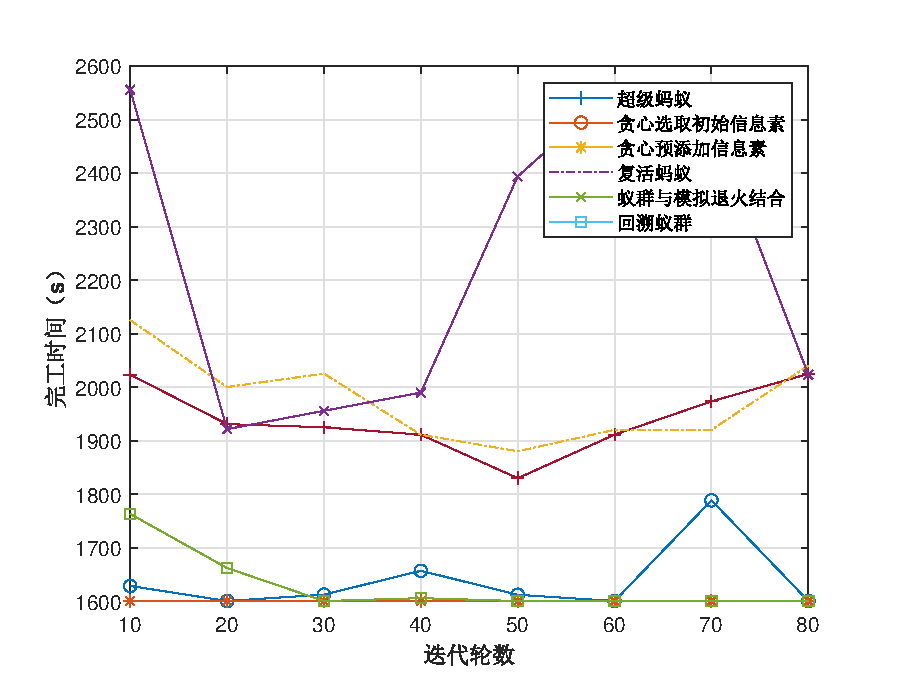
\includegraphics[scale=1.00,angle=0]{figures/test1.eps}\\
	\caption{蚁群算法各个优化思路迭代轮数与完工时间关系(10到80轮)}
\end{figure}

如上图所示,按迭代轮数与完工时间关系曲线的运动趋势可将6种优化思路分为3类:随迭代轮数增加,完工时间先递减后在较高值处振荡、完工时间始终在迪杰斯特拉解附近、随迭代轮数增加完工时间有收敛到迪杰斯特拉解的趋势。

关系曲线符合随迭代轮数增加,完工时间先递减后在较高值处振荡的优化思路有:超级蚂蚁、复活蚂蚁、蚁群与模拟退火结合

关系曲线符合完工时间始终在迪杰斯特拉解附近的优化思路有:贪心选取初始信息素、贪心预添加信息素

关系曲线符合随迭代轮数增加完工时间有收敛到迪杰斯特拉解的趋势的优化思路有:回溯蚁群

各种优化思路均对解产生了效果,单纯从解质量来看贪心选取初始信息素、贪心预添加信息素、回溯蚁群均能求解出接近迪杰斯特拉算法的解。
接下来将对各优化思路的类别进行分析。

\subsection{对随迭代轮数增加,完工时间先递减后在较高值处振荡的优化思路进行分析}
超级蚂蚁、复活蚂蚁、蚁群与模拟退火结合这三种思路随迭代轮数增加,完工时间先递减后在较高值处振荡。
将其与原始蚁群相比较,可以发现这三种优化思路都能够加快低迭代轮数时完工时间下降的速度。
复活蚂蚁机制的完工时间下降速度低于超级蚂蚁机制。
但是随着迭代轮数的继续增加,完工时间下降的趋势明显减缓,最终会在一个较高值附近振荡。
加入模拟退火机制的算法的振荡幅度显著高于其他两种机制,并且前期完工时间是从较高值快数下降的。

对于超级蚂蚁来说,如果发现更优的解,更优解会被添加上远高于其他解的信息素,前期几乎所有蚂蚁都会被引导上某条更优解。
但是基于上一节对第四章模型解分布的分析,最优解附近存在大量死锁,有走向最优解的蚂蚁很容易遇到死锁提前结束循迹。
因此即便使用超级蚂蚁,最优解上积累的信息素也会很快被其他互通的较差解超过。
算法无法收敛到最优解。

对于复活蚂蚁来说,前期完工时间下降快是因为提前结束循迹的蚂蚁被其他蚂蚁替代复活后,有效蚂蚁的数量大大增加,
实际上相当于增加了蚂蚁数量。
但是因为走向最优解并遇到死锁提前结束循迹蚂蚁会被走向较差解的蚂蚁替代,算法依然无法收敛到最优解。

对于模拟退火来说,在还未探索到较优解时,逐步提高后期蚂蚁,将避免算法局部收敛,因此算法前期波动会更大。
后期受第四章模型特殊的解分布的影响,拥有更高地位的蚂蚁反而会更剧烈地把解引导到互通的差解区域。
因此后期的解依然波动很大。

综上这三种机制并不适合求解类似第四章模型的时间Petri网。

\subsection{对完工时间始终在迪杰斯特拉解附近的优化思路进行分析}
贪心选取初始信息素、贪心预添加信息素这两种优化思路完工时间始终在迪杰斯特拉解附近。
这两种思路都和贪心的思想紧密相关。
有可能第四章模型本身适合使用贪心算法求解,因此需要排除贪心算法本身对解的影响才能分析蚁群算法效果。

使用贪心算法对第四章模型进行求解,结果如下:

变迁序列为:$t_{1}$->$t_{7}$->$t_{1}$->$t_{2}$->$t_{1}$->$t_{17}$->$t_{3}$->$t_{7}$->$t_{16}$->$t_{1}$->$t_{23}$->$t_{2}$->$t_{1}$->$t_{17}$->$t_{27}$->$t_{7}$->$t_{16}$->$t_{1}$->$t_{2}$->$t_{1}$->$t_{4}$->$t_{14}$->$t_{24}$->$t_{12}$->$t_{22}$->$t_{1}$->$t_{13}$->$t_{29}$->$t_{11}$->$t_{22}$->$t_{1}$->$t_{14}$->$t_{12}$->$t_{22}$->$t_{20}$->$t_{18}$->$t_{1}$->$t_{4}$->$t_{14}$->$t_{24}$->$t_{12}$->$t_{22}$->$t_{20}$->$t_{18}$->$t_{13}$->$t_{1}$->$t_{29}$->$t_{11}$->$t_{22}$->$t_{20}$->$t_{18}$->$t_{14}$->$t_{1}$->$t_{12}$->$t_{22}$->$t_{20}$->$t_{18}$->$t_{1}$->$t_{4}$->$t_{14}$->$t_{24}$->$t_{12}$->$t_{22}$->$t_{20}$->$t_{18}$->$t_{13}$->$t_{20}$->$t_{18}$->$t_{8}$->$t_{29}$->$t_{22}$->$t_{14}$->$t_{20}$->$t_{18}$->$t_{9}$->$t_{22}$->$t_{20}$->$t_{18}$->$t_{20}$->$t_{18}$->$t_{4}$->$t_{10}$->$t_{9}$->$t_{24}$->$t_{22}$->$t_{6}$->$t_{8}$->$t_{22}$->$t_{28}$->$t_{10}$->$t_{20}$->$t_{18}$->$t_{9}$->$t_{22}$->$t_{20}$->$t_{18}$->$t_{20}$->$t_{18}$->$t_{4}$->$t_{10}$->$t_{9}$->$t_{22}$->$t_{20}$->$t_{18}$

完工时间为:1600.8s

程序运行时间为:0.065s

变迁序列和完工时间均与迪杰斯特拉解一样,因此此网的贪心解就是最优解。

原模型为S3PR模型,本就适合最早加工策略的调度,因此使用贪心算法就能求出最优解。
破坏原模型的顺序结构,使其加工腔的晶圆可以重入得到网1 。

基于上文的分析,算法收敛到差解的主要原因是此模型存在死锁,因此需要研究算法在无死锁模型下的情况。
网1存在大量死锁,对网1进行死锁控制形成网2 。
对网1、网2使用100只蚂蚁的蚁群算法分别从10轮每次递增10轮直到80轮进行测试两种优化思路,观察完工时间。

网1的测试结果如下:

\begin{table}[H]
	\centering
	\caption{网1各优化思路完工时间与迭代轮数关系}
	\resizebox{!}{!}{
		\begin{tabular}{c|cccccccccc}
			\toprule
			\diagbox{优化思路}{完工时间(s)}{迭代轮数} & 10 & 20 & 30 & 40 & 50 & 60 & 70 & 80  \\
			\hline
			贪心选取初始信息素 & 2554.7 & 2124.5 & 2024.1 & 1973.7 & 1921.1 & 1973.7 & 1990.0 & 1973.7  \\
			贪心预添加信息素 & 2393.8 & 2024.5 & 2024.5 & 2024.1 & 1973.7 & 1920.7 & 1973.1 & 1921.1  \\
			\bottomrule
		\end{tabular}
	}
\end{table}

网2的测试结果如下:

\begin{table}[H]
	\centering
	\caption{网2各优化思路完工时间与迭代轮数关系}
	\resizebox{\linewidth}{!}{
		\begin{tabular}{c|cccccccccc}
			\toprule
			\diagbox{优化思路}{完工时间(s)}{迭代轮数} & 10 & 20 & 30 & 40 & 50 & 60 & 70 & 80  \\
			\hline
			贪心选取初始信息素 & 2040.5 & 2034.5 & 1911.5 & 1820.3 & 1788.9 & 1763.5 & 1662.4 & 1600.8  \\
			贪心预添加信息素 & 2554.7 & 2120.1 & 1973.7 & 1900.5 & 1820.3 & 1788.9 & 1700.5 & 1606.2  \\
			\bottomrule
		\end{tabular}
	}
\end{table}

\begin{figure}[H]
	\centering
	% Requires \usepackage{graphicx}
	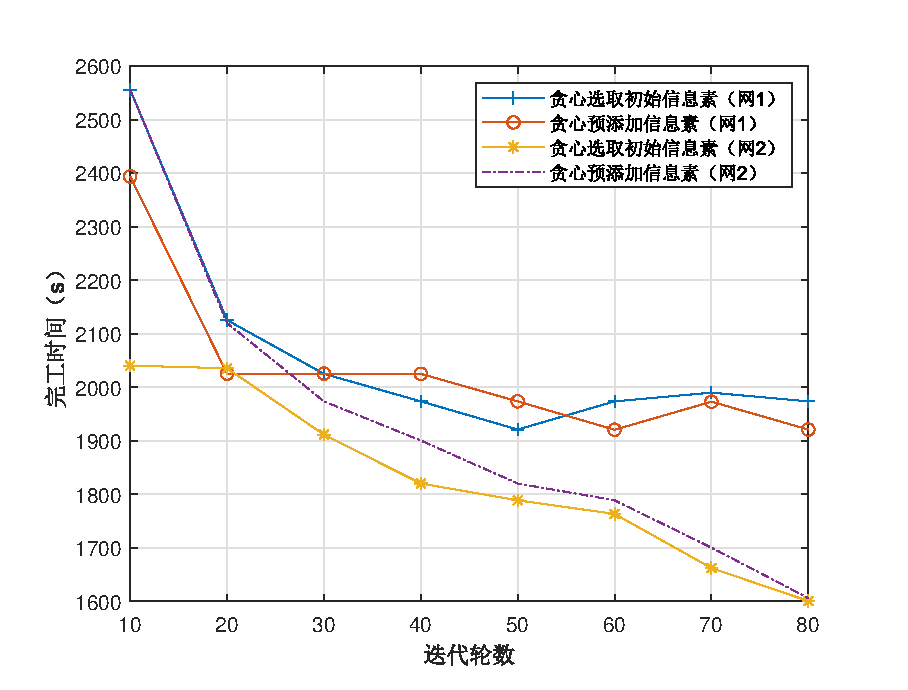
\includegraphics[scale=1.00,angle=0]{figures/test2.eps}\\
	\caption{贪心优化思路迭代轮数与完工时间关系(10到80轮)}
\end{figure}

如上图所示,如果不做死锁控制,加入贪心机制的蚁群算法依然无法收敛到最优解。
因此对于最优解附近有大量死锁的时间Petri网,这两种优化思路效果有限。但是如果在使用蚁群求解前,预先消除Petri网死锁,算法将会有很好的收敛效果。

\subsection{对随迭代轮数增加完工时间有收敛到迪杰斯特拉解的趋势的优化思路进行分析}
只有回溯蚁群机制一种优化思路能让算法随迭代轮数增加完工时间有收敛到迪杰斯特拉解的趋势。

本次测试回溯蚁群时蚂蚁寿命上限是使用统计平均寿命的方法实现的。
对静态蚂蚁寿命和最小蚂蚁寿命也在相同条件下进行实验,静态蚂蚁寿命设置为100 。

\begin{table}[H]
	\centering
	\caption{各寿命上限机制与完工时间与迭代轮数关系}
	\resizebox{!}{!}{
		\begin{tabular}{c|cccccccccc}
			\toprule
			\diagbox{蚂蚁寿命上限机制}{完工时间(s)}{迭代轮数} & 10 & 20 & 30 & 40 & 50 & 60 & 70 & 80  \\
			\hline
			静态蚂蚁寿命 & 2359.2 & 2120.1 & 1983.1 & 1900.5 & 1880.4 & 1780.5 & 1730.5 & 1616.2  \\
			最小蚂蚁寿命 & 2492.3 & 2020.4 & 2123.1 & 2124.7 & 2374.2 & 2522.5 & 2473.3 & 2554.7  \\
			\bottomrule
		\end{tabular}
	}
\end{table}

\begin{figure}[H]
	\centering
	% Requires \usepackage{graphicx}
	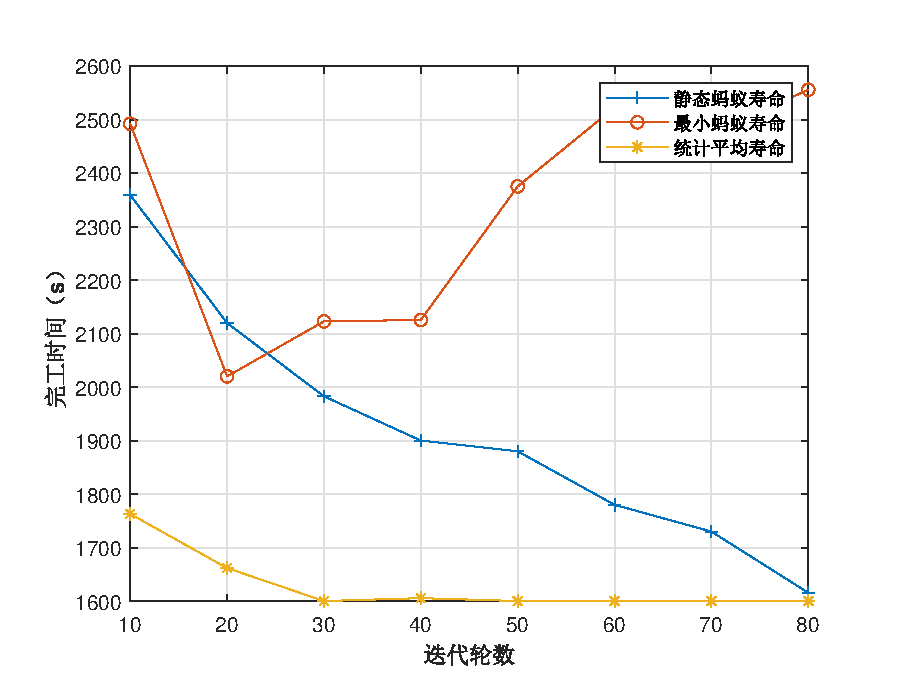
\includegraphics[scale=1.00,angle=0]{figures/test3.eps}\\
	\caption{不同蚂蚁寿命上限机制与完工时间关系(10到80轮)}
\end{figure}

如上图所示,静态蚂蚁寿命与统计平均寿命能够使算法收敛到最优解,但是最小蚂蚁寿命机制随着迭代轮数的增加,解的质量会恶化。

其原因可能是使用最小蚂蚁寿命机制时,算法后期的蚂蚁寿命上限过低,以至于蚂蚁失去回溯能力,无法走上死锁过多的路径。

统计使用最小蚂蚁寿命机制与统计平均寿命时,蚂蚁寿命上限与迭代轮数的关系。

\begin{table}[H]
	\centering
	\caption{各寿命上限机制与寿命上限与迭代轮数关系}
	\resizebox{!}{!}{
		\begin{tabular}{c|cccccccccc}
			\toprule
			\diagbox{寿命机制}{寿命上限}{迭代轮数} & 10 & 20 & 30 & 40 & 50 & 60 & 70 & 80  \\
			\hline
			静态蚂蚁寿命 & 83 & 24 & 10 & 1 & 1 & 1 & 1 & 1  \\
			统计平均寿命 & 167 & 201 & 123 & 25 & 12 & 15 & 10 & 13  \\
			\bottomrule
		\end{tabular}
	}
\end{table}

\begin{figure}[H]
	\centering
	% Requires \usepackage{graphicx}
	\includegraphics[scale=1.00,angle=0]{figures/test4.eps}\\
	\caption{不同蚂蚁寿命上限机制蚂蚁寿命上限与迭代轮数的关系(10到80轮)}
\end{figure}

如上图所示,使用最小蚂蚁寿命时,蚂蚁寿命上限很快降低到最小值,以至于后期蚂蚁几乎没有回溯能力。
但使用统计平均寿命时蚂蚁寿命上限最终收敛于12左右,依然具备一定的回溯能力,并且远小于直接配置静态寿命100,大大节约了程序运行时间。

\subsection{CPU数量对回溯蚁群算法速度的影响}
基于本章第1节对本蚁群算法流程的描述,本文所使用的蚁群算法为多线程算法。
所有蚂蚁均可并行地探索可达图,蚂蚁数量越多,在CPU数量不做限制时,算法将寻找到更多的解。
因此不论从解质量还是程序运行时间的角度看蚂蚁数量越多越好。

但是根据4.4.3.2节的实验数据,当蚂蚁数量在10以上时,再增加蚂蚁数量对解贡献就不大了。
而实际情况下CPU数量是有限的,线程切换时会有额外的CPU资源的开销,因此不宜设置过高的蚂蚁数量。

迪杰斯特拉算法是单线程算法,不会受到CPU数量影响,因此提升CPU数量无法减小程序运行时间。
在使用了m1 ultra的Mac Studio上使用迪杰斯特拉算法计算第四章建立的时间Petri网模型,程序运行时间为7.232s。
以此为基准,使用100只蚂蚁的蚁群算法迭代100轮,统计不同CPU数量下程序运行时间。

\begin{table}[H]
	\centering
	\caption{各寿命上限机制与寿命上限与迭代轮数关系}
	\resizebox{\linewidth}{!}{
		\begin{tabular}{c|cccccccccccc}
			\toprule
			CPU数量 & 11 & 12 & 13 & 14 & 15 & 16 & 17 & 18 & 19 & 20 \\ \hline
			程序运行时间(s) & 23.525 & 14.312 & 8.753 & 6.624 & 4.231 & 4.441 & 3.001 & 2.121 & 1.361 & 1.214 \\
			\bottomrule
		\end{tabular}
	}
\end{table}

\begin{figure}[H]
	\centering
	% Requires \usepackage{graphicx}
	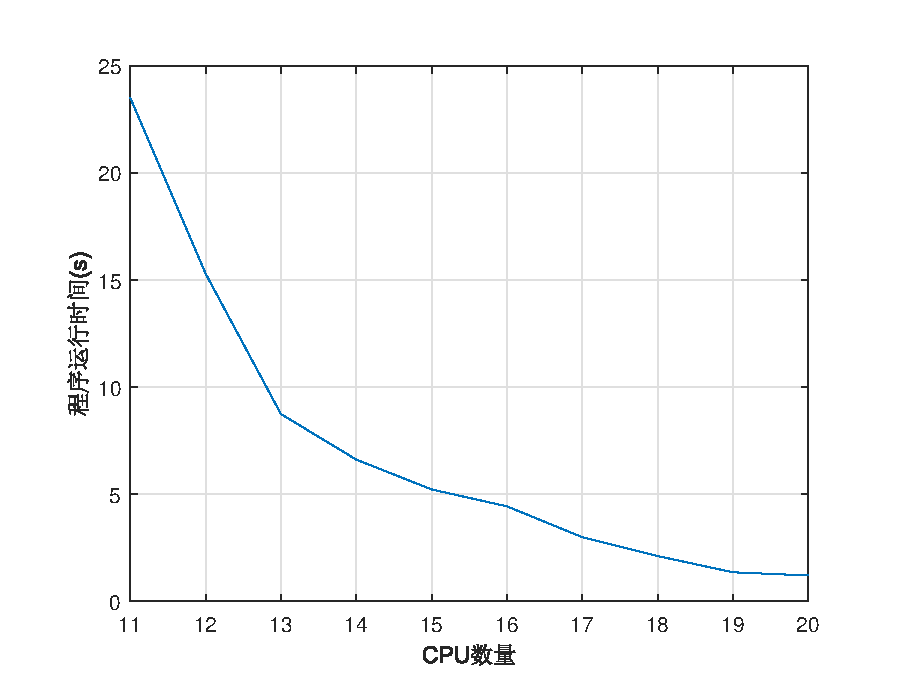
\includegraphics[scale=1.00,angle=0]{figures/test5.eps}\\
	\caption{蚁群算法不同CPU数量下程序运行时间}
\end{figure}

如上图所示,当开启14个CPU时,程序运行时间就已经优于迪杰斯特拉算法了,继续增加CPU数量能显著提升算法效果。

\section{本章小结}
本章提出了一种基于时间Petri网的蚁群算法,使用此算法求解上一章模型的调度策略,并与迪杰斯特拉算法相比较。
发现蚁群算法的解明显劣于迪杰斯特拉算法,
而且随迭代轮数增加,算法不能收敛。
于是基于实际情况,设计了6种优化方案,最终回溯蚁群策略效果明显。
% \chapter{总结与展望}
\section{总结}
晶圆制造系统是用于生产半导体芯片的设备和工艺的集合体。
它由多个工艺步骤组成,包括晶圆清洗、切割、涂覆、曝光、蚀刻、离子注入、金属沉积等。
晶圆制造系统通常由多个设备组成,包括晶圆清洗机、曝光机、蚀刻机、离子注入机、金属沉积机等。
这些设备通常由自动化系统控制,以确保工艺步骤的准确性和一致性。
本文使用Petri网对实际的晶圆制造系统进行建模,并设计蚁群算法求此系统进行调度。

本文第二章介绍了Petri网的基本理论,总结了各种调度算法。
并且梳理了一系列时间Petri网的相关知识。

第三章根据晶圆制造系统的特点,结合了第二章介绍的变迁时间网可库所时间网,提出了一种新的时间网子类,变迁库所时间网。
并且设计了一种此时间网变迁发射的时间计算流程,以保证变迁发射后系统时间尽可能短,以及一个用于计算各种Petri网模型的程序架构,供后续调度算法使用。
之后使用变迁库所时间网对一个实际的晶圆制造系统进行建模。

第四章使用蚁群算法对第三章建立的模型进行调度。
但发现调度结果不能收敛到最优解,通过对解的分析,从不同角度提出了6种优化思路,
最终回溯蚁群算法效果显著。
\section{展望}
\subsection{变迁库所时间网的进一步优化思路}
如果晶圆需要进入一系列的加工腔加工,并且规定此晶圆从进入第一个加工腔开始,必须在规定时间内完成加工,最直观的做法是有某套机制能够跟踪晶圆。
晶圆由托肯表示,各托肯在Petri网中是无法区分的。
因此之后可以设计并开发一套托肯编号机制。

实际的Petri网系统中,既有托肯表示晶圆,也有表示逻辑值,这类托肯在被变迁移动时所进入的库所是不同的,
并且实际系统中存在多个晶圆交换操作。
因此应该设计一套托肯移动的规则,以保证上述逻辑的正确。
\subsection{蚁群算法的进一步优化思路}
对于蚁群算法的进一步优化,可以从时间和空间两个方面入手。
减少算法的时间开销可以通过阻止蚂蚁探索无意义的标识实现;
减少空间开销可以设计更高效的数据结构来实现。
\subsubsection{全局时间禁忌表}
本文结合Petri网的实际情况,提出了回溯蚁群算法并取得了不错的成果。
蚂蚁能够回溯后便拥有了发现不可行解的能力。
如果将这批不可行解记录下来,下一轮蚁群循迹时提前禁止蚂蚁走上不可行解,将大大提高蚁群算法收敛速度。
不可行解由标识组成,因此可以使用一个新的集合存储这些标识。
此集合用于避免蚂蚁走上无意义的标识,功能与禁忌表相似,
因此将其命名为全局禁忌表。

而本算法是基于时间Petri网的,
此Petri网超过时间约束也会引发死锁,
此类死锁受时间因素影响不能简单的判定为不可行解。

综上全局禁忌表存储的应该为一系列的键值对,键为不可行解中的标识向量,
值应为一系列的充分条件。
如果蚂蚁探索到的标识满足这一系列的条件,则意味着继续探索不可能到达终点标识。
这一系列的充分条件会随着蚁群的探索一步步细化,逼近充要条件。
\subsubsection{实现禁忌表新的数据结构}
如果将Petri网的标识向量编码为二进制串,有一种比哈希表更高效的数据结构,二元决策图可以以更低的空间开销存储二进制信息。
蚁群算法为多线程算法,更为适合在GPU上运行,GPU的显存带宽远高于内存带宽,但通常来说显存大小不如内存,并且显存与内存通信需要消耗时间。
因此可以使用布隆过滤器在显存和内存间做一层中间层,把显存中长期未处理过的标识转移入内存中。
内存与硬盘间也可以使用相似的逻辑,这样可以极大提升存储标识的数量。
\chapter{绪论}
本章主要阐述了气井智能管控系统的研究背景及意义,对国内外油气数字化现状进行了调研。进一步解释了对气井进行分类、产量预测和开关井推荐的必要性。最后对论文主要研究内容和组织结构进行了简要说明。
\section{研究背景和意义}
天然气是世界上广泛使用的能源。2022年,世界天然气消费量3.94万亿立方米,全球油气勘探开发投资支出4934亿美元,其中我国全国天然气
消费量3646亿立方米,进口天然气1503亿立方米\cite{chinaGasGOv}。在我国的能源资源中有举足轻重的地位。

随着计算机技术的快速发展和软件技术的高速迭代,利用计算机技术来应用于传统行业已经十分有必要。
尽管我国原材料工业数字化转型不断走向纵深,但仍面临计算机技术应用于产业不够深入等问题\cite{workplanForPetrochemical}。油气行业面对气井智能分析的需求,迫切的需要利用计算机技术进
行数字化的建设和发展。本文将使用计算机方法来对气井进行分类、对气井产气量预测、根据预测结果进行开关井推荐,并以此为基础设计一个包含数据管理和智能分析的气井智能管控系统。

目前,已经有相当多的学者开展了气井分类方
面的研究,但当前绝大多数的分类方法需要基于
现场管理认识,给出指定的分类界限,对管理经验要
求较高的同时,还具有相当的主观性\cite{SYZC202104015}。同时,苏里格气田是典型的三低(低渗透、低压力、低丰度)气田,不仅单井产量低,产量递减快,压力下降快,且积液严重,大多数为间歇性气井\cite{KTSY202306014}。
对于该气田而言,不同井的特征随时间变化的差异很大,相对于基于传统特征的分类方法,采用时间序列聚类分析方法可以深入分析气井随时间变化的产气量,允许用户精准地识别出不同生产条件下气井的行为模式。时间序列聚类能够基于实际的生产动态,而不仅仅是静态和动态特征,提供更个性化、适应性更强的气井预测算法,从而可以根据预测结果来提供开关井策略。这有助于最大化生产效率,减少液体积累带来的问题,优化生产过程,从而在不同的生产阶段维持气井的最佳运行状态,提高整体的生产效能。

气井产能预测是气田开采过程中最基本的任务之一。常用的传统的预测气井产量的方式有两种:预测气井的绝对无阻流量和通过递减曲线分析来预测产量。气井的无阻流量指的是在气井井底流压降低到0.1MPa时,气井的产气量。实测无
阻流量指的是将气井彻底敞开,当井底流动压力和大气压保持相同时,测量产气量, 此即为实测无阻流量。 该方法被认为是不合理的 , 原因在于气管尺寸会影响到结果的准确
性。而且操作过程中形成的气体会有严重的消耗,在水的锥进以及砂子颗粒的磨损作用下气井会受到影响。递减曲线分析方法依赖于简化假设和历史生产数据,这可能不完全反映复杂的地质和工程条件,特别是在非常规气藏中。此外,该方法忽略了井筒和地层之间的非均质性,需要长期的生产历史来形成准确的分析,且未考虑经济因素,从而可能导致对未来产量的预测不够准确或适用。

鉴于传统预测方法有诸多弊端,很多学者采用机器学习如时间序列预测等方法来预测气井产量,目前油气产量时间序列预测的研究大多是同步时间序列预测,问题描述为:已知属性(Source)和预测目标(Target)在每一步相对应,且已知属性时间序列长度和预测目标时间序列长度相等时计算产量。同步时间序列预测实际上是对未测量数据的计算,因此,能够应用的场景有限。
本文通过将静态变量,现在已知的未来变量和过去的动态变量融合到同一个网络中,可以进行多时间尺度的预测。

在对气井进行预测后,企业可以根据预测结果来进行开关井推荐,使得生产决策更加数据驱动,确保资源的有效利用。气井的产量通常受到管网两端压力差的限制。当管网两端的压力差较大时,气井的产量会增加;而当压力差较小时,气井的产量会减少。相应地,开关井操作会改变管网两端的压力差。一般情况下,开井会导致管网两端的压力差减小,而关井则会导致压力差增大。此外,当管网两端的压力差发生变化时,会对气井的稳定性产生影响。特别是在压力差较小时,气井的稳定性容易受到影响。因此,在开关井控制中,需要综合考虑管网两端的压力差和气井的稳定性因素,制定最优的开关井策略,以确保气井的生产稳定性。
本文采用果蝇优化算法,根据用户期望产量,基于管网模型计算理论值与计算值的差值,来作为开关井选择的标准。

同时,陕西某油田企业不同部门的数据杂乱无章,数据格式不统一,内容不共享,用户往往需要维护多个平台的账号信息,学习每个平台的使用方式,使用Excel等格式文件在各平台间导入导出数据,导致管理十分混乱。随着企业战略发生变化,需要高度整合自身资源,避免未来的智能分析工作陷入瓶颈,系统设计了数据连接和数据管理功能。

受企业委托,本文提出了基于机器学习的气井智能管控系统,通过现有理论完成气井分类、产气量预测和开关井工作,并根据企业需求设计了气井智能管控系统。系统不仅包括气井分类、产气量预测和开关等推荐等智能分析的内容,还根据企业数据杂乱管理混乱的痛点
设计了数据连接、数据管理、可视化展示和用户权限管理等功能。本文系统已完成一期交付,正处于线上试用阶段,目前运行状况良好。

\section{国内外研究现状}
\subsection{时间序列聚类算法}
时间序列聚类可以很好地用于趋势分析和预测,在股票市场分析、气象预报等领域已经有了广泛应用。时间序列聚类与常规的数据聚类方法存在显著区别,主要体现在处理数据的方式上。其中一种方法是基于形状的聚类,它通过调整时间序列在时间轴上的延展和收缩来匹配两个序列的形状。C.Ratanamahatana等于2006年提出了一种混合聚类算法,这种算法先根据动态时间弯曲(Dynamic Time Warping, DTW)的相似性度量方法将时间序列分成不同的小组,然后利用K-Means和K-Medoids算法进行聚类。另一种方法是基于特征的聚类,其中V. Hautamaki和其他学者在2008年介绍了一种方法,该方法首先将每个时间序列转换成等长的特征向量,然后使用欧几里得距离来实现聚类。这些方法都是为了更好地解决时间序列数据的特殊性,以揭示数据中隐藏的模式和结构。
时间序列聚类的关键在于如何准确测量不同时间序列之间的相似性。这个概念最初由R.Agrawal及其同事在1993年提出,并迅速成为数据挖掘领域的重要问题。在寻找时间序列之间相似形状的传统方法中,欧氏距离和动态时间规整(DTW)距离是常用的指标。近年来,研究人员探索了新的方法来改进这一过程。例如,S. Chu在2002年基于DTW开发了一种名为迭代深化动态时间规整(IDDTW)的方法。此外,为了提高时序聚类的通用性、精确度和效率,John Paparrizos与Luis Gravano在2016年引入了一种新的基于形状的距离度量(SBD),这种方法不受时间伸缩和平移的影响,增强了其适用性和扩展性。
\subsection{时间序列预测算法}
在时间序列分析的历史进程中,自回归模型(AR),首次提出于1927年,为统计学在时间序列预测领域的应用奠定了基础。随后,自回归积分移动平均(ARIMA)模型的发展,标志着基于统计学的预测方法进入了一个新阶段,ARIMA模型因其综合了自回归、积分和移动平均的特性而成为后续研究的核心。此后的模型大多在此模型的基础上进行改进。
然而这些模型的建立和预测精度在很大程度上依赖于参数选择,而不当的参数设定可能导致预测效果不佳,尤其是在面对复杂和动态变化的数据时。因此,尽管统计学模型在时间序列分析领域内有着长久的应用历史和理论基础,但在实际应用中仍需要细致的参数调整和模型选择。
机器学习在处理时间序列数据时表现的十分优秀。支持向量机是一种二分类模型,但可以通过多个支持向量机进行回归预测。在时间序列预测中,支持向量机常用的核函数包括线性核函数、多项式核函数和径向基核函数。
随机森林是一种集成学习算法,其基本单元为决策树。在时间序列预测中,随机森林可以对多个决策树进行集成,从而提高预测的准确性。集成学习是一种将多个弱分类器组合成强分类器的机器学习算法。在时间序列预测中,集成学习可以通过组合多个基模型来提高预测的准确性。常用的集成学习[11]算法包括Adaboost、Bagging和随机森林等。其中LightGBM是一个基于Boosting的集成树模型,由微软亚洲研究院开发并开源,其通过构建梯度提升决策树来预测时间序列。该框架特别适合处理大规模数据集,因为它采用了直方图优化算法和叶子优先的树增长策略,显著降低了内存消耗和提升了计算速度。LightGBM还支持分类特征和连续特征,使其能够灵活处理各种类型的时间序列数据。此外,通过应用自动特征选择和过拟合防止策略,LightGBM能够生成准确且鲁棒的时间序列预测模型。
此外,还有一系列神经网络算法也应用于时间序列预测领域。循环神经网络(RNN)是1990年由Elman首次提出,用于处理序列数据。RNN通过在模型中设置隐藏层来保存过去的状态,并将其作为后续输入的一部分,以此来捕获时序信息。然而,RNN在处理长期依赖问题时表现不佳,因此发展出了长短期记忆网络(LSTM)和门控循环单元(GRU)等改进型网络。LSTM通过引入控制门机制来改善长时间依赖的捕获,而GRU则简化了LSTM结构,降低了模型复杂度。此外,为了解决RNN只能利用单向数据的限制,双向循环网络(Bi-LSTM)被提出,使模型能同时利用过去和未来的信息。自2017年由Vaswani等人提出Transformer模型以来,其已成为深度学习领域的革命性创新。该模型通过引入自注意力机制,有效改进了对长期依赖性的学习,显著提升了自然语言处理等领域的性能。尽管其在长序列预测上存在挑战,如二次时间复杂度,但其并行计算能力和高效的自注意力机制使其在多个领域得到广泛应用,展现出优越的性能。此外,最新研究也表明,注意力机制在时间序列预测方面相比传统模型展现出更好的效果。如TFT(Temporal Fusion Transformers),其结合了LSTM和自注意力机制的优势,能够有效地捕获时间序列中的长期和短期依赖性。TFT 的核心是一个多头自注意力机制,它允许模型同时关注过去、现在和未来的时间点,提高了预测的准确性和解释性。此外,TFT 通过其可变选择网络 (Variable Selection Networks) 部分,能够自动识别并选择对预测任务最相关的输入特征,这不仅提高了模型的效率,也增加了模型结果的可解释性。
\subsection{机器学习在油气产量的应用}
前文可知,有多种机器学习算法应用于时间序列预测领域,其在油气田产量预测领域的应用也十分广泛。
Hui团队考虑了地质和操作变量,测试了线性回归、人工神经网络、梯度提升树以及极端树四种不同的模型,最终发现极端树模型在预测页岩气产量方面最为有效,并据此提出了提高产量的建议。
Liao团队开发了一个基于数据挖掘的模型用于致密油产量预测,通过敏感性分析确认了关键变量,并确定随机森林为最适合的模型。
Niu等人应用了随机森林、支持向量机、K最邻近和梯度提升树四种机器学习方法来预测油田的最终采收率,其中支持向量机的表现最优,并指出早期生产数据对预测结果有重要影响。
Li等人的研究聚焦于使用机器学习方法优化压裂产能预测,经过变量筛选后,发现随机森林模型提供了最佳预测结果,并基于此提出了施工优化建议。
Morozov及其团队执行了一个全面的累积油产量预测研究,涵盖了从数据处理到模型比较的整个过程。他们测试了多种机器学习技术,包括支持向量机(SVM)、K最近邻(KNN)、人工神经网络以及多种基于树的算法,如决策树、随机森林、极端随机树、CatBoost、梯度提升树和极端梯度提升树。在进行了详细的超参数调整和模型比较后,他们发现CatBoost模型提供了最准确的预测结果。
Schuetter及同事对不同的预测模型进行了评估,包括简单线性回归、随机森林、支持向量机、梯度提升树和多维克里金方法,用以预测油井的生产指标。他们还利用决策树分析了各个模型中特征的重要性,以区分高产和低产油井,并对这些变量的重要性进行了探究。
Meng及同事研究了页岩气吸附行为的预测,建立了人工神经网络、随机森林、支持向量机和极端梯度提升四种机器学习模型。他们将这些模型的预测效果与传统的基于压力和密度的等温模型以及压力温度统一模型进行了比较。研究结果显示,机器学习模型能够提供准确的预测,并克服了温度和岩石类型的限制,其中极端梯度提升模型表现最佳。
这段内容总结了多个研究项目,每个都专注于使用不同的机器学习技术来预测油气产量。Kubota团队提出了一个适应性强的线性模型来准确预测油井的产油率和产液率,强调机器学习可以补充传统油气工程工具。Li等人利用主成分分析和神经网络识别了影响页岩气产量的主要因素,并提出了提高产量的策略。Lin团队通过BP神经网络和数据分析方法,预测了生产能力,并确定了最优的生产参数。Han等人探讨了不同模型在预测累积产气量方面的效能,发现深度神经网络最有效。Amirian和同事们展示了使用Levenberg-Marquardt和反向传播方法构建的模型在预测准确度上的优势,并强调了超参数和数据量在模型训练中的重要性。Wang等人的研究通过深度神经网络模型分析了影响短期和长期产油量的关键因素,强调了超参数的重要性。
Chaikine和Gates使用混合卷积递归神经网络(C-RNN)来预测多级压裂井的五年累积产量。他们发现这种模型在预测单个油井产量时不仅准确度高,而且当整合多个井的数据时,预测的准确性会显著提高。
Panja及其团队通过使用人工神经网络(ANN)、最小二乘支持向量机(LSSVM)和二阶多项式响应面法(RSM)来建立一个考虑时间和速度限制的油井采收率预测模型。他们的研究结果显示,RSM和LSSVM在预测原油采收率方面比ANN更有效,且LSSVM在预测油气比方面展现出更高的准确性。
以上研究皆表明机器学习方法可以在油气产量预测上有很好的应用且效果优于传统方式。
\section{论文研究内容}
结合油田企业数字化转型的问题背景分析以及相关国内外研究现状,本文基于时间序列预测领域相关的技术方案设计了基于机器学习的气井智能管控系统。该系统的智能分析模块包括气井分类、产气量预测和开关井推荐算法。本文的主要内容如下:
(1)给出了一种基于改进的K-Shape时间序列聚类算法的气井分类算法,用于解决气井分类的问题。首先,本文描述了气井产气的原理,分析了对不同气井进行分类管控必要性。然后对取得的气井数据进行数据清洗,建立了气井时间序列聚类
的模型。最终实验结果显示,该方法可以有效地对气井进行分类。
(2)为了帮助企业有效规划气井的开发和生产过程,本文分别针对不同的气井类型进行产气量预测,给出了一种基于transformer的气井产量预测算法。首先使用滑动窗口的方法对第三章已经清洗好的数据进行数据预处理,然后根据不同的协变量
对输入的历史时刻和未来时刻的特征经过一系列变换,得到一个抽象的表征,
然后分别输入到 Encoder 和 Decoder 中。Encoder 部分使用 GRU 网络来编码历史时刻
的信息,输出一个固定长度的向量,表示整个历史序列的含义。Decoder 部分使用自
注意力机制来解码未来时刻的预测值,每个预测值都是根据之前所有时刻的加权结
果得到的。通过该算法,系统可以预测出未来时刻气井的产气量。根据产气量预测的结果,本文采用果蝇优化算法来对气井的开关井策略进行推荐。
(3)设计了一个气井智能管控系统,依据该企业各种数据杂乱无章的痛点,使用Apache Hudi对煤
企业的数据进行采集和存储,使用ClickHouse提供强大的数据分析能力,搭建一个
数字化平台系统,帮助企业进行数据的存储、管理和分析。支持用户在系统中进行气井的智能分析,并支持数据的可视化展示,根据油田部门的部门体系设计了用户和权限管理功能。
\section{论文组织结构}
根据课题内容,论文主要组织结构如图\ref{fig:paperStructure}所示。
\begin{figure}[H]
    \centering
    \caption{论文主要章节结构图}
    \label{fig:paperStructure}
\end{figure}
根据图\ref{fig:paperStructure}的主要章节结构安排,本文主要由六个章节组成,各章节组织结构如下:

第一章:绪论。本章主要阐述了基于机器学习的气井智能管控系统的研究背景及研究意义,并对国内外当前的时间序列聚类、时间序列预测和机器学习在油气产量的应用现状进行了描述,最后简要阐述了论文的主要研究内容和论文的组织结构。

第二章:基础理论和相关技术。本章详细介绍了论文涉及的相关理论和相关技术,其中包括使用的算法技术、算法模型、数据库技术等。

第三章:基于改进的 K-Shape 时间序列聚类算法的气井分类算
法。本章为了识别具有相似生产行为和特性的气井群体,了解不同气井的行为模式,优化生产策略,实现更有效的资源管理和分配,提出了一个基于改进的 K-Shape 时间序列聚类算法的气井分类算
法。从算法流程和思路对算法模型进行介绍,对企业内部的数据进行清洗并验证,最终验证了模型的有效性。同时,通过第四章,先对气井分类后再做产气量预测,可以提高预测的准确性,它允许模型更好地理解和适应每个聚类内序列的特定特征和动态变化。

第四章:基于transformer的气井产量预测算法。
\chapter{相关技术概述}
\section{相关算法}
\subsection{K-Shape时间序列聚类算法}
\label{section2.1.1}
K-Shape算法\cite{yang2017k}是一种基于形状的时间序列聚类算法,用于将相似的时间序列分为同一类。其基本思想是通过对时间序列进行自动化预处理和转换,然后使用基
于形态的距离SBD(\textbf{\underline{S}}hped-\textbf{\underline{B}}ased \textbf{\underline{D}}istance)来计算时间序列之间的相似
度,从而实现聚类。K-Shpae使用归一化的互相关系数$NCC_{c}$(Normalized Cross-Correlation Coefficient)来描述两个时间序列的形状相似性。$NCC_{c}$是
一种衡量两个时间序列在不同时刻相似程度的度量方法。通过计算一个序列与另一个序列的滑动版本之间的相似性,我们可以识别它们之间的潜在关系。在时间序列 \( x_t \) 
和 \( y_t \) 中,\( x_t \) 可以通过滑动窗口 \( s \) 来计算与 \( y_t \) 的互相关 \( CC_w(x_t, y_t) \),其中 \( s \) 是滑动窗口的大小,
\( x_t' \) 是 \( x_t \) 的滑动版本。当 \( s > 0 \) 时,\( x_t' \) 是 \( x_t \) 向右滑动 \( s \) 个单位的结果,
即 \( x_t' = (0, \ldots, 0, x_1, x_2, \ldots, x_{m-s}) \);当 \( s < 0 \) 时,\( x_t' \) 是 \( x_t \) 向左滑动 \( |s| \) 个单位
的结果,即 \( x_t' = (x_{-s}, \ldots, x_m - 1, x_m, 0, \ldots, 0) \)。具体表达式如公式\eqref{eq:shift}所示:
\begin{equation}
    x_(s) = 
        \begin{cases} 
        \overbrace{(0, \ldots, 0)}^{|s|}, x_{1+s}, x_2, \ldots, x_{m-s}, & s \geq 0 \\
        x_{1-s}, \ldots, x_{m-1}, x_m, \underbrace{(0, \ldots, 0)}_{|s|}, & s < 0 
        \end{cases}
    \label{eq:shift}
\end{equation}
\( CC_w(x_t, y_t) \) 的计算公式如公式\eqref{eq:NCC1}与公式
\eqref{eq:NCC2}所示。
当 \( w \leq m \) 时,
\begin{equation}
CC_w = \sum_{k=1}^w x'_k \cdot y_{k+m-w}
\label{eq:NCC1}
\end{equation}
当 \( w > m \) 时,
\begin{equation}
CC_w = \sum_{k=1}^{2m-w} x'_{k-m+w} \cdot y_k
\label{eq:NCC2}
\end{equation}
其中,\( m \) 是序列的长度,\( w \) 是滑动窗口的宽度。这允许我们在不同的时间滞后下计算序列 \( x_t \) 和 \( y_t \) 之间的相似度。
如图\ref{fig:NCC}所示,当$x_t$右移2步时\( CC_w(x_t, y_t) \)达到最大序列对齐。
\begin{figure}[H]
    \centering
    % Requires \usepackage{graphicx}
    \includegraphics[scale=0.3,angle=0]{figure/NCC.jpg}\\
    \caption{移动时间序列}
    \label{fig:NCC}
\end{figure}
不同的时间序列数据可能在量级上差异巨大,需要对其归一化调整到相同的尺度。归一化是数据预处理中常用的技术,主要用于调整数据集中变量的尺度,使
其具有统一的标准。这通常通过将每个数据点减去平均值并除以标准差来实现,以便转化后的数据集具有零均值(\( \mu = 0 \))和单位方差
(\( \sigma^2 = 1 \))。这种转换被称为标准化或Z得分归一化。对于一个给定的时间序列 \( x_t \),其归一化后的值 \( x_t' \) 可以通过以下
公式计算得出:

\begin{equation}
x_t' = \frac{x_t - \mu}{\sigma}
\label{eq:normal1}
\end{equation}

其中,\( \mu \) 是原始时间序列 \( x_t \) 的均值,\( \sigma \) 是其标准差。这个过程确保了不同的数据集可以在相同的比例上进行比较和分析。K-Shape
算法采用系数归一化$NCC_c = \frac{CC_w(x,y)}{\|x\|\|y\|}$的方式对\( CC_w(x, y) \)进行归一化。互相关序列除以各个序列自的几何平均值。归一化后,
SBD的计算公式如式\eqref{eq:SBD}所示:
\begin{equation}
    SBD(x_t, y_t) = 1 - \max_w \left( \frac{CC_w(x_t, y_t)}{\|x_t\| \cdot \|y_t\|} \right)
    \label{eq:SBD}
\end{equation}
当两段时间序列重合越多,他们形状越相似,$CC_w(x_t, y_t)$就越大。对比所有可能位置的相似度值,取最相似的$max(NCC_c)$,再通过$1-max(NCC_c)$得到
SBD。表明了当两条时间序列越相似时,SBD越小。由于归一化以后的$NCC_c$在[-1,1]之间,因此SBD的值在[0,2]之间。当SBD=0时,意味着两条序列一模一样。
但是用上述方法对序列之间距离做对比时,时间复杂度为$O(m^2)$,当序列长度较长时,复杂度会很高,计算量也会很大。为解决这一问题,作者通过傅立叶变换的
方法,将序列从时域转换为频域再进行比较。此时,离散傅里叶变换(Discrete Fourier Transform, DFT)及其逆变换(Inverse Discrete Fourier Transform, IDFT)发挥了
至关重要的作用。DFT将时域信号转换为频域表示,而IDFT则实现了反向过程,允许序列从频域返回到时域。在K-shape聚类算法中,DFT和IDFT的运用可以描述如下。
给定时间序列 \( x_t \) 和 \( y_t \),首先应用DFT将这些序列转换为它们的频域表示 \( F(x_k) \) 和 \( F(y_k) \)。在频域中,通过简单地把原序列
的DFT结果,应用IDFT,我们可以有效地计算序列间在不同滑动窗口 \( w \) 下的互相关 \( CC_w(x_t, y_t) \)。
离散傅立叶变换和逆变换的数学表达式公式\eqref{eq:DFT}为:
\begin{equation}
    F(x_k) = \sum_{r=0}^{m-1} x_r e^{-\frac{2 \pi i r k}{m}}, \quad k = 0, \ldots, m - 1
    \label{eq:DFT}
\end{equation}
\begin{equation}
    F^{-1}(x_r) = \frac{1}{m} \sum_{k=0}^{m-1} F(x_k) e^{\frac{2 \pi i k r}{m}}, \quad r = 0, \ldots, m - 1
    \label{eq:IDFT}
\end{equation}
根据这些变换,互相关可以通过公式\eqref{eq:ccf}计算:
\begin{equation}
    CC_w(x_t, y_t) = F^{-1}(F(x_t) \times F(y_t))
    \label{eq:ccf}
\end{equation}
通过傅立叶变换的方式计算互相关的算法复杂度为\( O(m \log m) \),这使其计算SBD时在计算性能上十分高效,可以显著加快整个聚类过程。
K-Shape需要在簇内找到最优簇心$c_k^* = [c_1 \quad c_2 \quad \ldots \quad c_m]$使得簇$P_t$内所有序列$x_t$与$c_k^*$的SBD距离总和最小。其
等价的最大化问题为公式\eqref{eq:ck1}。
\begin{equation}
    c_k^* = \arg\min_{c_k} \sum_{x_t \in P_k} SBD(x_t, c_k)
    \label{eq:ck1}
\end{equation}
根据K-Shpae迭代的特性,将公式\eqref{eq:ck1}与公式\eqref{eq:SBD}结合,并将$c_k$标准化,可得到最终的簇心计算公式为式\eqref{eq:ckfin},其中$\mathbf{S} = \sum_{x_t \in P_k} x_t \cdot x_t^T$
\begin{equation}
    c_k^* = \arg\max_{c_k} \frac{c_k^T \cdot \mathbf{S} \cdot c_k}{c_k^T \cdot c_k}
    \label{eq:ckfin}
\end{equation}
此时,问题转化为了经典的瑞利商(Rayleigh Quotient)问题。只要求得矩阵$\mathbf{S}$的最大特征值,$c_k$的解就是$\mathbf{S}$最大特征值对应的特征向量。
\subsection{GRU}
\subsection{Transformer}
\chapter{基于改进的K-Shape时间序列聚类算法的气井分类算法}
在气井开采初期,气井一经投入使用就会打破气藏的静态平衡,诸如产量、压力和产物性质等关键参数便会随之变动。随着开采活动的进行,气水关系会愈加错综复杂。产水量将持续攀升,
低压井和产水井的数量不断增长,不同气井之间的差异会日益增大。这些因素会进一步增加气井的生产管理难度。为提高管理效能,企业需利用历史产量数据对气井进行有效分类。将
表现出相似生产特性的气井进行归类和分析,以帮助揭示它们的共同生产模式。使得企业能够迅速评估气井的生产状况,掌握关键生产特征,进而及时规划出针对性强的管理策略和治
理行动,以确保气井的顺畅运作。本章根据基于改进的分数阶时间序列聚类算法,根据气井的历史产量数据,对气井进行分类。首先对企业提供的报表数据进行整理和清洗,去除掉
报表中的冗余数据并将需要的信息批量提取出来。在获取了产量相关的序列后,使用改进的K-Shape时间序列聚类算法来对气井进行分类。
\section{问题分析}
企业气田的地质条件十分复杂,是典型的“低渗透、低压力、低丰度”气田。其单井产量小、压降速率快,随着气田不断进行规模开发,单井井数逐年增加,集气站也在不断的增大。
随着开采活动的不断进行,间歇井(气井按照固定的开关制度进行生产的气井)数量的也在逐步递增。气井在开采过程中,产量会随着井底污染、地层压力、地层渗透率、地层有效厚度
等的变化。不同气井产量随时间的变化差异巨大。因此,通过对气井产量进行时间序列聚类,可以将历史产量特性相似的井分为一类进行管理。帮助企业在后续开采、产气量预测
以及对间歇井的开关井策略制定时,根据类别分别制定方案。基于此需求,本章采用改进的K-Shape时间序列聚类算法,通过SBD来度量两变量之间的相似性,再根据数据的特征指定
初始簇心,通过迭代的方式不断更新,最终得到气井分类的结果。
\section{问题描述}
在气井产量的时间序列聚类分析中,我们的目标是将历史产量数据分组,以揭示不同气井的生产行为和潜在模式。具体而言,每个气井的时间序列数据可以表示为 \( X_i = \{x_{i1}, x_{i2}, \ldots, x_{im}\} \),其中 \( m \) 代表了时间序列的长度,即观测周期的总数。我们有 \( N \) 个这样的时间序列,形成了一个时间序列集合 \( X = \{x_1, x_2, \ldots, x_N\} \),我们的目标是将这些序列聚类到 \( k \) 个不同的类别中。
在聚类分析中,每个类别可能代表着不同的气井种类,正处在高产期和衰退期的井之间的时间序列差异巨大。假设k=3(但实际应用中需要根据肘部法则来确定最优的k值)则种类可以预先定义为类别 \( Y = \{0,1,2\} \)。因此,我们的任务是定义一个映射函数 \( f: X \to Y \),它可以将每个时间序列分配到这些预定义的类别中。
\section{基于改进的K-Shape时间序列聚类算法的气井分类算法}
\subsection{算法流程}
在传统的K-Shape聚类算法中,初始参考中心的选择是通过从样本集中随机挑选k个样本来进行的。这种随机选择方法可能会导致算法收敛于次优解,且每次运行结果都不一致,导致聚类结果不稳定。尤其是当数据集包含噪声或者离群点时。随机选取的初始中心可能不代表数据的真实结构,导致最终的聚类结果缺乏可解释性和准确性。此外,当样本集规模庞大时,随机选择方法可能导致算法收敛速度缓慢,影响聚类效率。
为了确定合适的聚类,通常采用多次实验的方法。本文结合领域知识和数据特点给出了一种改进策略:即根据数据特征选取初始中心点。具体如下:根据气井的历年累计产量,平均产量,
峰值产量的统计结果,对气井进行排序,并将其划分为k个区间,在每个区间内抽取中间的气井作为初始中心点。这样的方式可以使得初始的中心点更符合数据分布,从而实现
提高算法运行的稳定性。算法的流程图如图\ref{fig:K-Shape}所示。
\begin{figure}
    \centering
    % Requires \usepackage{graphicx}
    \includegraphics[scale=0.3,angle=0]{figure/K-Shape.jpg}\\
    \caption{基于改进的K-Shape时间序列聚类算法的气井分类算法流程图}
    \label{fig:K-Shape}
\end{figure}
初始报表的数据复杂且混乱,需要我们对其进行数据清理和整理,以形成一张规范的报表。在此基础上可以获取完整的产量数据,我们再根据第2章的方法对其进行归一化处理。然后
通过上文的方式选取初始参考中心。接下来,我们将通过不断的迭代更新簇心的方式来寻找最终的气井分类结果。这个过程将一直持续,直到簇心不再发生变化或者达到了预设
的最大迭代次数。最终,我们将得到一个高质量的气井分类结果。
\subsection{数据处理与分析}
原始数据集为单井日报文件,所给原始数据集时间跨度为:2012年8月3日至2022年8月15日,储存格式为一月的数据储存在一张excel多表中,一年共12张多表,每个
多表包含一月的数据,其中每日数据记录在一张excel表中,表中包含信息有所属井丛,井号,配产,生产时间(日累,月累,其中月累从2014年4月引入),油压,
套压(从2016年9月起开始引入),井口温度,注醇量(以井丛为单位),产气量(日产,月累,年累,历年年累),投产日期,备注(开关井信息)等。为进行批量读取处
理,需要先按照数据格式对所有报表进行划分,划分需考虑的因素包括不同的表头,报表的不同组织形式,不同的日期记录格式,剔除不需要的表(如一些影响批量读取的
总结性信息。如2012年的数据格式记录较为混乱,8,9两月的单井日报单井记录为了一个excel文件,10月,11月,12月三个月份的数据,由3个excel包含了各自月份的数据。

\chapter{基于transformer的气井产量预测算法}
在气井的全生命周期任务中,气井产量预测可以帮助企业有效规划气井的开发和生产过程,确定最佳的生产速率,以避免资源浪费和确保气井的长期稳定产出。同时,
准确的产气量预测有助于企业评估气井的经济价值,从而做出更加明智的投资决策,比如决定是否继续开发新的气田或是对现有气井进行增产操作。在制定策略时,了解
未来的产气量可以帮助企业更有效地分配资源,比如人力、资金和设备,确保这些资源被投入到最有价值和最需要的地方。并有助于在有风险的情况下识别潜在的生产下
降风险和其他相关风险,使企业能够及时调整策略以降低损失。气井产气量预测是根据气井的生产动态历史数据,对气井未来一段时间内的产能做出准确评估。过去比较广泛
的进行产量预测的方法为预测气井的绝对无阻流量或者通过下降曲线分析的快速方法来匹配生产率-时间历史数据。但是这些现有的用于非常规储量估算的产量递减评估技术
具有潜在的局限性和一些特定假设,如对于间歇生产气井难以进行预测,这可能导致估计错误。本文采用时间序列预测的方式,目前油气产量时间序列预测的研究大多是同步
时间序列预测,应用场景有限。例如:不能实现使用井的静态参数及已知生产曲线预测未来生产曲线,也不能结合训练好的模型来优化生产设计。基于这些痛点,本章借鉴
了TFT的算法,同时根据企业的专家经验设计了网络模型,完成了气井产气量的时间序列预测任务。
\section{问题分析}
气井产量预测要求根据不同气井的历史产气量数据,构建预测模型;在推理阶段,模型能够对任一指定气井未来一段时间内的单日产气量做出预测。

在时间序列预测中,协变
量(covariates)是指与时间序列相关的其他变量。这些变量可以影响时间序列的行为和变化,因此在时间序列预测中使用协变量可以提高预测的准确性。协变量可以是任
何与时间序列相关的变量,包括经济指标、天气数据、人口统计数据等。例如,假设我们正在预测某个城市未来一周的销售额。此时,可以考虑将天气数据作为协变量,因为
天气可能会影响人们购买某些产品的决策。

气井产量预测任务可以抽象为一个多时间序列预测问题(约1000个时间序列),使用变量包括静态协变量(气井号,井丛号,集气站号,气井类别),随时间变化的协变量
(Time-dependent Inputs),可以细分为过去可知,未来不可知的协变量(Past-observed Inputs),如油压,套压,井口温度,以及过去和未来都可知的协变量
(Apriori-known Future Inputs),如气井已经生产的天数,每日开井时间。此处,每日开井时间是一个影响产气量的重要因素,因为若开井时间为0,则产气量必定
为0。未来时刻的开关井时间受人工调控开关井的影响,是可知的,因此可以设置为过去和未来都可知的协变量。
\section{问题描述}
\subsection{单井产气量预测问题描述}
对于单个气井,其输入是气井一段时间的产量数据及对应的气井动态数据。对于单井一段时间内的数据,将其记为
\begin{equation}
    \left\{\left(x^1_{\delta}, x^1_{\rho}, x^1_{\sigma}, x^1_{\tau}, x^1_{h}, Y^1_{\phi}\right), \left(x^2_{\delta}, 
    x^2_{\rho}, x^2_{\sigma}, x^2_{\tau}, x^{2}_{h}, Y^2_{\phi}\right), \ldots, \left(x^T_{\delta}, x^T_{\rho}, x^T_{\sigma}, 
    x^T_{\tau}, x^{T}_{h}, Y^T_{\phi}\right)\right\}
    \label{eq:singlewell}
\end{equation}
其中\( N \)表示气井数据的总时间长度,其中上标$i$表示时刻$i$,下标表示不同的特征,分别如下所示:油压\( \delta \)、套压\( \rho \)、
井口温度\( \sigma \)、投产天数\( \tau \)、每日开井时间$h$、日产量$\phi$。则问题可以定义为:基于气井过去一段时间内的油压\( \delta \)等数据来预测气井未来一段时间内的产量,记要预测的未来时间步长$t$。形式化
地描述如公式\eqref{eq:sinpredic}所示。输入为。
\begin{equation}
    \begin{aligned}
        \left\{\left(x^1_{\delta}, x^1_{\rho}, x^1_{\sigma}, x^1_{\tau}, x^1_{h}, Y^1_{\phi}\right), \left(x^2_{\delta}, 
        x^2_{\rho}, x^2_{\sigma}, x^2_{\tau}, x^{2}_{h}, Y^2_{\phi}\right), \ldots, \left(x^T_{\delta}, x^T_{\rho}, x^T_{\sigma}, 
        x^T_{\tau}, x^{T}_{h}, Y^T_{\phi}\right), \left(x^{T+1}_{\tau}, x^{T+1}_{h}\right),\ldots, \left(x^{T+t}_{\tau}, 
        x^{T+t}_{h}\right)\right\}
    \end{aligned}
    \label{eq:sinpredic}
\end{equation}
输出为$\left\{ y^{T+1}_{\phi}, y^{T+2}_{\phi}, \ldots, y^{T+t}_{\phi} \right\}$。

对于时序数据预测问题,需要将一整条数据依据时间点划分为训练数据和测试数据,然后需要设置训练数据步长与滑动步长,从而生成多个样本。因此为将问题转换为时间
序列问题,需设置新的符合并对问题作进一步地定义。需要将记训练数据输入步长为$T$,$T$通常大于等于要预测的时间步长$t$,记滑动步长为$s$,记训练数据和测试数
据的划分时间点为$N_0$,记
\subsection{多井产气量预测问题描述}
现有产气量预测方法多为针对某一单一气井的建模,应用价值有限。每个气井的产量主控因素可能有较大差别,且很多参数是无法量化的,无法加入到机器学习中,带来了
较大的不确定性。因此,通过某一单一气井时间序列数据训练出的机器学习模型往往无法针对其他气井使用。

同时,对于本企业提供的气井数据集而言,一共包含1000余口气井的时间序列数据。一方面,要针对单一气井构建不同的时间序列模型是不现实的,单井的数据量是有限的,且部分气井仅具
有极少量数据,无法据此构建机器学习/深度学习模型,且模型过多会导致通用性差,难以管理等问题。另一方面,使用所有气井的数据集进行训练可以捕捉到不同气井之
间具有的相似的生产规律,提高了模型泛化性,实现了对多气井产气量预测的统一建模。

本文的多气井产气量预测在单井产气量预测的基础上添加一系列静态协变量(包括气井号,井丛号,集气站号和气井类别),并针对第三章得到的不同类别的气井生成特定类别的预测结果。因此多气井产量预测模型在
考虑了气井预测模型的泛化性的基础上又不失特殊性,从而实现了气井产量的高效预测。
\section{算法框架}
根据上文所述内容,需要根据气井的历史数据信息来预测气井的未来产量。本文借鉴了TFT的框架,并根据企业的气井数据特征来对TFT的模型进行了一些改进。具体
的算法框架如图\ref{fig:TFTprogess}所示。
\begin{figure}[H]
    \label{fig:TFTprogess}
    \caption{基于transformer的气井产量预测算法流程图}
\end{figure}
本章提出的气井产量预测算法具体分为以下几个步骤:
(1)气井数据提取:本章使用企业提供的气井数据,并在第\ref{cha:data}章中对气井数据进行了数据清洗,使得其可以直接在接下来进行数据处理。

(2)气井数据预处理:使用滑动窗口对气井数据进行处理,接下来对数据进行无量纲化处理,将所有特征缩放至$[0,1]$之间。最终把得到数据集用于后续模型的训练、验证和测试。

(3)获取气井类别:根据第三章的方式对气井进行分类,以根据气井在地质特征、井深、压力水平和历史产量等不同条件下分类的结果分别进行预测。

(4)使用基于transformer的方式对每类气井分别进行预测:根据气井不同的协变量,将输入的历史时刻和未来时刻的特征经过一系列变换,得到一个抽象的
表征,然后分别输入到Encoder和Decoder中。Encoder部分使用GRU网络来编码历史时刻的信息,输出一个固定长度的向量,表示整个历史序列的含义。
Decoder部分使用自注意力机制来解码未来时刻的预测值,每个预测值都是根据之前所有时刻的加权结果得到的,这样可以提高模型的准确性。
\section{数据处理及分类}
\label{sec:datafoc}
气井的数据在第\ref{cha:data}章已经选取了日期,集气站号,井序号,日产时间,井口压力(油压),套压,井口温度,日产量和投产时间等数据存储在了一
个名为GasProductionOri.csv的文件中。

但是此时的到的每条时间序列都过长,直接建模可能会由于计算资源的限制而变得不可行。为了统一输入输出格式,
降低模型复杂度和计算开销,本文使用滑动窗口技术将
训练数据切割为固定长度。滑动窗口模式是进行序列预测问题处理的最常用也是最有效方式,通过控制窗口的大小,可以调整参与预测的历史数据的数量。其模型如
图\ref{fig:slidewindow}所示。
\begin{figure}[H]
    \label{fig:slidewindow}
    \caption{滑动窗口数据分段示意图}
\end{figure}
如图\ref{fig:slidewindow}所示,设置滑动间隔为1,使用固定大小为4的滑动窗口,对气井的时间序列进行划分。在取出样本序列后,每个样本分段的数据差异大且复杂,
未经标准化处理的样本分段会导致机器学习模型的学习速度十分缓慢,甚至无法更新模型参数。同时,由于不同分段之间的差异,数值较大的分段可能会对模型的决策过程产生
不成比例的影响,导致模型偏向于这些数据,从而影响预测结果的准确性。我们需要对每个样本分段进行无量纲化处理,将所有特征放缩至$[0,1]$之间,即
\begin{equation}
    y = \frac{x - \text{min}}{\text{max} - \text{min}}
\end{equation}
其中$min$为该分段中的最小值,$max$为该分段中的最大值。

气井会因为它们的地理位置、地质构造、开采历史和技术等因素而表现出不同的产量特性。直接在所有气井数据上建立预测模型的话,模型就会过于复杂,难以捕捉到每一种类型气井的特点。而分类后,为每一类气
井建立模型可以简化问题,使得模型更容易泛化,减少过拟合的风险。同时,通过基于改进的K-Shape时间序列聚类算法对气井进行分类以后,可以将具
有相似产量特征的气井分为一组,使得预测模型能够专注于这些相似特征,从而提高预测准确性。第三章将气井分为 类,本章将分别对其进行产量预测。
\section{算法主要设计策略}
如图\ref{fig:TFT}所示,为基于transformer的气井产量预测算法的模型结构图。
\begin{figure}
    \label{fig:TFT}
    \caption{基于transformer的气井产量预测算法的模型结构图}
\end{figure}
由图中可知,网络模型主要由门控残差网络、输入层、时间特征处理层、时域注意力层、position-wise前馈层以及分位数预测层组成。
\subsection{门控残差网络}
\label{cha:GRN}
由于输入与目标之间的关系是未知的,对于预测结果而言,到底需要什么程度的非线性处理是一项巨大的挑战。非线性层过多会出现梯度消失或梯度爆炸的问题,因此,有时
需要简化模型来处理问题。为了让模型只在需要的时候才灵活地应用非线性地方式处理数据,我们提出了门控残差网络来处理数据。门控残差网络的输入为主输入$\mathbf{a}$
和一个可选的上下文向量$\mathbf{c}$。具体操作如下所示:
\begin{equation}
    GRN_{\omega}(\mathbf{a}, \mathbf{c}) = \text{LayerNorm}(\mathbf{a} + GLU_{\omega}(\boldsymbol{\eta}_1))
\end{equation}
其中:
\begin{equation}
    \boldsymbol{\eta}_1 = \mathbf{W}_{1,\omega} \boldsymbol{\eta}_2 + \mathbf{b}_{1,\omega}
\end{equation}
\begin{equation}
    \boldsymbol{\eta}_2 = \text{ELU}(\mathbf{W}_{2,\omega} \mathbf{a} + \mathbf{W}_{3,\omega} \mathbf{c} + \mathbf{b}_{2,\omega})
    \label{eq:eta2}
\end{equation}
上式中,ELU是指线性激活函数,$\eta_1 \in \mathbb{R}^{d_{\text{model}}}$, $\eta_2 \in \mathbb{R}^{d_{\text{model}}}$ 是中间层,
LayerNorm是于2016年被提出的标准归一化,$\omega$ 是表示权重共享的索引。当$\mathbf{W}_{2,\omega} \mathbf{a} + \mathbf{W}_{3,\omega} \mathbf{c} + \mathbf{b}_{2,\omega} \gg 0$时,
ELU激活函数将作为恒等函数,而当$\mathbf{W}_{2,\omega} \mathbf{a} + \mathbf{W}_{3,\omega} \mathbf{c} + \mathbf{b}_{2,\omega} \ll 0$ 时,ELU激活函数产生一个固定的输出,直接触发线性层的行为。我们使用基于门控线性单元 (GLUs)的组件门控层来
提供灵活性,以抑制数据集中不需要的任何体系结构。假设 $\boldsymbol{\gamma } \in \mathbb{R}^{d_{\text{model}}}$ 是输入,GLU的形式为:
\begin{equation}
    GLU_{\omega}(\boldsymbol{\gamma }) = \sigma(\mathbf{W}_{4,\omega} \mathbf{\boldsymbol{\gamma }} + \mathbf{b}_{4,\omega}) \odot (\mathbf{W}_{5,\omega} \mathbf{\boldsymbol{\gamma }} + \mathbf{b}_{5,\omega}),
\end{equation}
其中 $\sigma(\cdot)$ 是sigmoid激活函数,$\mathbf{W}_{(\cdot)} \in \mathbb{R}^{d_{\text{model}} \times d_{\text{model}}}$ 是权重,$\mathbf{b}_{(\cdot)} \in \mathbb{R}^{d_{\text{model}}}$ 是偏置,
$\odot $ 是元素的Hadamard乘积。GLU允许模型控制GRN对原始输入$\mathbf{a}$的贡献程度--如果必要,GLU的输出可以都接近于0,以便抑制模型非线性
的贡献。对于没有上下文向量$\mathbf{c}$的实例,GRN简单地将上下文输入视为0(即在\eqref{eq:eta2}中,$\mathbf{c}=0$)。
\subsection{输入层}
本模型将融合了多种数据源。具体地由图中可知:输入层包括三种类型的变量。最左侧的$S$是静态变量,包括气井号、井丛号、集气站号和气井类别。从$x_{t-k}$到$x_t$代表的是从过去$k$时刻已知
,但未来不可知的随时间变化的变量,包括井口温度,油压,套压,日产量等。最右侧的$x_{t+1}$到$x_{t+\tau_{max}} $代表的是从过去$t-k$到未来$t+\tau_{max}$时刻
都可知的随时间变化的变量,包括已经投产的天数,每日开井时长等。

其中静态变量$S$需要经过静态协变量编码器来整合来自静态元数据的信息。具体地,本文使用\ref{cha:GRN}所展示的门控残差网络来编码产生上下文向量$\mathbf{c}_h$
,$\mathbf{c}_h$将传入时间特征的局部处理层作为GRU的初始输入。
\subsection{时间特征处理层}
在时间序列的数据中,重要的点例如异常、变化点或者周期性模式一般都是根据他们周围的值来识别的。通过编码时间序列能够在序列中记忆和使用先前的信息,增强局
部上下文,从而提高基于注意力架构模型的性能。本文将采用序列到序列层来进行时间序列编码,TFT使用LSTM来对时间序列进行编码,但是LSTM参数量相对较多,其包
括更多的门控单元。这会导致在训练和推理过程中需要更多的计算资源,特别是气井数据集的规模较大。尽管LSTM设计用来更好地捕捉长期依赖关系,但有时候它会
受到梯度消失或爆炸的影响,导致难以有效地学习长期依赖,这可能需要额外的技巧或者调整来解决。基于以上痛点,本文使用GRU来对时间序列进行编码。
GRU具有更简单的结构,它合并了LSTM的遗忘门和输入门,因此参数数量较少。这使得GRU在训练和推理过程中的计算效率更高。且其有更快的训练速度,。这使得在大规
模数据集上进行实验和调整参数时更加高效。我们将过去的输入序列$\bm{\xi}_{t-k:k}$提供给编码器,将未来的输入序列$\bm{\xi}_{t+1:t+\tau_{max}}$
提供给解码器。使用GRU生成一组均匀的时间特征,作为下一阶段的输入,用$\phi (t,n)$来表示,
其中$\phi(t,n) \in {\phi(t, -k), \ldots, \phi(t, T_{\text{max}})}$,$n$是位置指标。这种方式也可以完美处理观测到的过去和未来的输入不同而
存在的差异。同时,为了让静态数据也参与到时间序列变量的编码中,我们使用$\mathbf{c_h}$上下文向量初始化第一个GRU的隐藏状态。在此处也使用门控跳跃链接:
\begin{equation}
    \tilde{\bm{\phi}}(t, n) = \text{LayerNorm}\left(\tilde{\bm{\xi}}_{t+n} + \text{GLU}_{\tilde{\phi}}(\bm{\phi}(t, n))\right)
\end{equation}
其中$n \in [ -k, \tau_{\max}]$是位置指标。
\subsection{时域注意力层}
在进行GRU编码后,我们采用自注意力来学习不同时间步之间的长期关系。传统的多头注意力每个头使用不同的值,仅通过权重注意力本身并不能指示特定特征的重要性,此处
在传统多头注意力的基础上共享V。具体如下:
一般来说,注意力机制基于键矩阵\( K \in \mathbb{R}^{N \times d_{\text{attn}}} \)和查询矩阵\( Q \in \mathbb{R}^{N \times d_{\text{attn}}} \)
之间的关系对值\( V \in \mathbb{R}^{N \times d_v} \)进行缩放:
\begin{equation}
    \text{Attention}(Q, K, V) = A(Q,K)V
\end{equation}
其中$A()$是一个归一化函数,\( N \) 是进入注意力层的时间步数(即 \( k + t_{\text{max}} \))。常用的选择是缩放点积注意力:
\begin{equation}
    A(Q, K) = \text{Softmax}\left(\frac{QK^T}{\sqrt{d_{\text{attn}}}}\right)
\end{equation}
为了提高注意力机制的学习能力,Vaswani于2017年提出了多头注意力,使用不同的头针对不同的表示子空间:
\begin{equation}
    \text{MultiHead}(Q, K, V) = [H_1, \ldots, H_m]W_H
\end{equation}
\begin{equation}
    H_h = \text{Attention}(QW^Q_{(h)}, KW^K_{(h)}, VW^V_{(h)})
\end{equation}
其中\( W^K_{(h)} \in \mathbb{R}^{d_{\text{model}} \times d_{\text{attn}}} \), \( W^Q_{(h)} \in \mathbb{R}^{d_{\text{model}} \times d_{\text{attn}}} \), \( W^V_{(h)} \in \mathbb{R}^{d_{\text{model}} \times d_v} \) 
是针对键、查询和值的头特定权重 \( W_H \in \mathbb{R}^{m \cdot h \times d_{\text{model}}} \) 用于将所有头输出合并。
为了展示特定特征的重要性,做出的修改如下:
\begin{equation}
    \text{InterpretableMultiHead}(\mathbf{Q}, \mathbf{K}, \mathbf{V}) = \tilde{\mathbf{H}} \mathbf{W}_h
\end{equation}
\begin{equation}
    \begin{aligned}
        \mathbf{\tilde{H}} &= \tilde{A}(\mathbf{Q}, \mathbf{K}) \mathbf{V} \mathbf{W}_v, \\
        &= \left\{ \frac{1}{m_H} \sum_{h=1}^{m_H} A(\mathbf{Q} \mathbf{W}_Q^{(h)}, \mathbf{K} \mathbf{W}_K^{(h)}) \right\} \mathbf{V} \mathbf{W}_v, \\
        &= \frac{1}{m_H} \sum_{h=1}^{m_H} \text{Attention}(\mathbf{Q} \mathbf{W}_Q^{(h)}, \mathbf{K} \mathbf{W}_K^{(h)}, \mathbf{V} \mathbf{W}_v),
    \end{aligned}        
\end{equation}
式中:$\mathbf{W}_v \in \mathbb{R}^{d_{\text{model}} \times d_v}$是跨所有头共享的值的权重,$\mathbf{W}_h \in \mathbb{R}^{d_{\text{attn}} \times d_{\text{model}}}$
用于最终的线性映射。$\tilde{A}(\mathbf{Q}, \mathbf{K})$允许我们通过分析一组注意力权重来进行简单的可解释性研究。

在进行了时间特征处理层之后,我们应用注意力层。将所有的时间特征组合成单一的矩阵即$\bm{\varPhi }(t) = \left[ \bm{\phi} (t, -k), \ldots, \bm{\phi }(t, \tau_{\text{max}}) \right]^T$
并在每个时间点($N = \tau _{max} + k + 1$)应用时域注意力:
\begin{equation}
    \mathbf{B}(t) = \text{InterpretableMultiHead}(\mathbf{\varPhi }(t), \mathbf{\varPhi }(t), \mathbf{\varPhi }(t)),
\end{equation}
生成了$\mathbf{B}(t) = \left[ \mathbf{\beta }(t, -k), \ldots, \mathbf{\beta }(t, \tau_{\max}) \right]$。在自注意力层之后,增加了一个额外
的门控层来促进训练:
\begin{equation}
    \boldsymbol{\delta}(t, n) = \text{LayerNorm}(\boldsymbol{\phi }(t, n)) + \text{GLU}_{\boldsymbol{\delta}}(\boldsymbol{\beta}(t, n)).
\end{equation}
\subsection{position-wise前馈层}
对自注意力层应用额外的非线性处理,此处依然使用门控残差网络:
\begin{equation}
    \boldsymbol{\psi}(t, n) = \text{GRN}_{\boldsymbol{\psi}}(\boldsymbol{\delta}(t, n))
\end{equation}
其中$ \text{GRN}_{\boldsymbol{\psi}}$的权重在整个层中共享。此处还应用了一个跳过整个transformer块的残差连接,为序列到序列层提供了直接的路径。
倘若不需要额外的复杂性,就可以得到一个更简单的模型。如下所示:
\begin{equation}
    \tilde{\boldsymbol{\psi}}(t, n) = \text{LayerNorm}(\tilde{\boldsymbol{\phi}}(t, n)) + \text{GLU}_{\tilde{\boldsymbol{\psi}}}(\tilde{\boldsymbol{\psi}}(t, n))
\end{equation}
\subsection{分位数预测层}
借鉴了MQRNN框架的思路,本文采用分位数回归预测作为模型的输出方式。具体来说就是回归模型在对目标产量进行预测的时候不只预测$y$的一个期望值$\hat{y}$,
而是预测出$y$的概率分布中不同百分位数(如10\%,50\%,90\%)的值。分位数预测是根据上一步输出的线性变换生成的:
\begin{equation}
    \hat{\boldsymbol{y}}(q, t, \tau) = \mathbf{W}_q \tilde{\boldsymbol{\psi}}(t, \tau) + \mathbf{b}_q
\end{equation}
本文采用联合最小化分位数损失来训练模型,并将所有的分位数方法相加,具体如式\eqref{eq:loss}所示。
\begin{equation}
    \mathcal{L}(\Omega, \mathbf{W}) = \sum_{y_t \in \Omega} \sum_{q \in \mathcal{Q} } \sum_{\tau=1}^{\tau_{\max}} \frac{\text{QL}(y_t, \hat{\boldsymbol{y}}(q, t - \tau, t), q)}{M_{\tau_{\max}}}
    \label{eq:loss}
\end{equation}
其中$\text{QL}(y,\hat{y},q)$为分位数损失,具体定义如下:
\begin{equation}
    \text{QL}(y, \hat{y}, q) = q(y - \hat{y})_+ + (1 - q)(\hat{y} - y)_+,
\end{equation}
在式\eqref{eq:loss}中,$\Omega$是包含M个样本的训练数据,$W$表示模型的权重,$\mathcal{Q}$是分位数的集合(用户可自行指定,本文使用$\mathcal{Q} = \{0.4, 0.6\}$)。
\section{实验对比分析}
\subsection{数据集描述与环境说明}
基于transformer的气井产量预测算法会在第\ref{sec:datafoc}节提供的数据集上进行验证。本次实验的硬件环境为处理器Inter(R) Xeon(R) Silver 4261 cpu @ 2.10Hz,
显卡GeForce RTX 3090,内存256G,磁盘1T,操作系统采用Windows 10,开发环境为Pycharm,Python环境为Anaconda-4.12.0 python=3.9。
\subsection{评估指标}
为了验证本章所提出的基于transformer的气井产量预测算法的有效性,使用两个指标用于评估。其中一个是平均绝对误差(Mean Absolute Error, MAE),其可以衡量
预测值与实际值之间的平均绝对偏差。公式如式\eqref{eq:MAE}所示。
\begin{equation}
    MAE(y, y') = \frac{1}{n} \sum_{i=1}^{n} |y_i - y'_i|
    \label{eq:MAE}
\end{equation}
另一个常用误差指标为累计产量的相对误差,公式如式\eqref{eq:RCPE}所示。
\begin{equation}
    RCPE = \frac{\sum_{i=1}^{n} |y_i| - \sum_{i=1}^{n} |y'_i|}{\sum_{i=1}^{n} |y_i|}
    \label{eq:RCPE}
\end{equation}
上面两式中,$i$表示索引,用于遍历数据集中的每一个数据点。例如,如果我们有一个包含多个观测值的数据集,$i$就用来表示这些观测值的序号,从第一个观测值
到第$n$个观测值。$y$表示真实值,也就是实际产量,$\hat{y}$表示预测值,也就是通过模型预测得到的产量。
\subsection{实验结果与对比分析}
(1)对比实验
根据前文所述,本问题需要同时对1000余口气井构建时间序列预测模型,且问题包含多种类型的协变量,因此选用基于注意力机制的seq2seq模型,lightGBM模型和TFT这三个可以
解决这类问题的模型来进行对比实验。为了展示各算法的预测性能,选出3口井的产量数据作为测试集进行测试,分别是:SN0016-05, SN0004-04,SN0012-10。这3口
井的近期平均产量分别位于大于2,1到2之间,小于1区间(单位:$10^4m^3$)。如表\ref{ta:compareTFT}所示。
\begin{table}[H]
    \centering
    \caption{不同算法预测结果对比表}

\end{table}

\chapter{实验结果}
\section{气井分类实验结果}

\section{产气量预测实验结果}
\chapter{系统设计与实现}
本章根据企业的的痛点需求,设计并实现了一个气井智能管控系统,系统包含了第三章的
结合RFM与核密度估计的气井分类算法和第四章的基于transformer的气井产量预测算法及开关井推荐算法。
主要功能有数据连接,数据管理和智能分析等模块。
\section{系统需求分析}
\subsection{总体需求分析}
某油田企业作为行业的重要参与者,面临着诸多数字化建设方面的挑战。随着气井数量的增多以及老井的管理难度加大,需要按照气井全生命周期管理理念,引入机器学习、大数据分析等前沿技术,提升气井生产管理的研究决策质量和效率。其在数字化建设中主要遇到下列问题:

首先,过去企业缺乏对数据的智能分析,主要依赖于传统的、基于经验的决策方式,这种做法未能充分利用现有数据资源,从而导致生产计划不稳定、资源利用效率低下等一系列问题。此外,尽管企业过去积累了大量的数据,但由于缺乏有效的智能分析工具,这些宝贵的数据资源并未被充分利用,造成了资源的极大浪费。

其次,随着智能分析需求的不断深入,需要引入地质、钻探、环境等数据等时,该企业发现其所涉及的气井数据呈现出高度的多样性和复杂性。地质数据和钻探数据的来源及格式多样,加之企业内部是按职能划分的垂直部门结构,导致不同部门间存在较大的生产数据格式差异。同时,企业在软
件应用上高度分散,各业务单元采用
不同的软件系统存储数据,这极大地增加了在智能分析过程中进行数据处理的难度。

针对以上问题,该企业迫切需要建立一个软件结构合理的气井管控系统。该系统应能够对气井数据进行智能分析,利用机器学习的方式科学地指导未来决策。
同时可以有效地整合、存储和管理各类数据,包括来自不同软件和不同格式的数据。
通过建立这样一个系统,该油田企业能够通过数据的高效共享与分析,来为企业的决策提供科学依据和参考。

本系统面向的是油田企业的员工,他们的计算机基础较为薄弱,期望使用简单易懂的界面,通过简单的操作加载数据并获取所需结果。具体包含了以下需求:

(1)拥有智能分析功能:可以对数据进行智能分析。系统可以对气井数据进行分类、产气量预测和开关井推荐,提升气井及生产管理的研究决策质量和效率。

(2)可以对多元异构数据对接和导入:可以从不同来源采集数据并统一存储在数据湖中,保留原始数据信息。可以处理来自不同系统、不同格式的数据,可以进一步的智能分析提供更加全面的数据资源。

(3)具有数据管理的功能:可以对导入到数据湖的数据进行持久化保存。此外,系统支持数据集定时和周期任务的调用,使数据处理过程更加自动化和高效。

通过对系统进行总体的需求分析,对气井智能管控系统进行模块划分。
具体包括以下三个模块:数据连接、数据管理和智能分析。其模块划分图
如图\ref{fig:allmodules}所示。
\begin{figure}[H]
    \centering
    \includegraphics[width=.5\linewidth]{figure/systemincludemodles.pdf}
    \label{fig:allmodules}
    \caption{气井智能管控系统模块划分图}
\end{figure}
\subsection{系统功能性需求}
(1)智能分析

智能分析是系统最重要的部分,目前的模块包括第二章和第三章的气井分类、产气量预测和开关井推荐操作。其中产气量预测可以让用户选择气井号,选择预测步长和开始预测日期,同时还提供模型效果检验功能。开关井推荐可以根据用户想要达到的产量目标、压力差阈值和用户想要
排除的不参与生产的井来进行开关井的推荐。
\begin{figure}[H]
    \centering
    \includegraphics[width=.7\linewidth]{figure/智能分析用例图.pdf}
    \caption{智能分析用例图}
    \label{fig:analyusecase}
\end{figure}

(2)数据连接

在气井智能管理系统中,数据连接模块负责从多种数据源中采集和导入数据。油田企业的数据通常存储在关系型数据库(如MySQL、SQL Server)中,也可能以CSV文件的形式存储。此外,油田数据还涉及到非关系型数据库(如HBase)和流式消息中间件(如Kafka)等数据源。
数据连接管理模块设计具有良好的扩展性,能够根据需要灵活添加新的数据源。在油田数据连接管理中,用户首先选择目标数据源,然后创建相应类型的数据连接,并填写相关的连接信息,如数据库地址、用户名、密码等。完成连接信息后,用户可以将连接信息持久化保存,以便后续使用。
其用例图如图\ref{fig:dataconnectionusecase}所示。
\begin{figure}[H]
    \centering
    \label{fig:dataconnectionusecase}
    \includegraphics[width=.7\linewidth]{figure/数据连接用例图.pdf}
    \caption{数据连接用例图}
\end{figure}

(2)数据管理 

数据管理包括对数据集进行目录管理、数据集管理以及对数据集更新。其中数据集管理包括新建数据集、浏览数据集等。
\begin{figure}[h]
    \centering
    \includegraphics[width=.6\linewidth]{figure/数据管理用例图 .pdf}
    \caption{数据管理用例图}
    \label{fig:datamaucase}
\end{figure}
新建数据集可以通过数据库数据集,SQL数据集,文件数据集,上传文件等方式创建。其中数据库数据集是直接从已有的数据连接中选择的数据库中的表作为数据集。
SQL数据集可以通过SQL语句和从已有的数据连接中获取返回结果作为数据集。
文件数据集表示用户导入本地Excel文件,上传为数据集。数据集更新主要包括对数据集手动更新或者通过定时/周期任务来更新。
上传文件表示用户导入本地其他类型的文件,上传为数据集。目录管理可以查看数据的各种结构关系。具体如\ref{fig:datamaucase}所示。

上文中对系统进行了总体需求分析和功能需求分析,但除了对必要的功能进行需求分析之外,气井智能管控系统还需要在响应时间、易用性等非功能的需求方面保障用户的使用体验。

(1)响应时间

在实际开发中,一般要求系统处理请求并返回结果的总耗时在一定时间内。对于系统的响应时间,通常会要求在3000毫秒内完成。此处要求一般任务可以在500ms内完成。
本项目最耗时的部分为数据导入、更新和智能分析部分。此处要求单个数据集的导入时间不超过0.5h,并可允许同时有5个气井数据进行导入/更新;智能分析模块中,气井预测可能耗时相对较久,此处要求气井预测时间不超过10s,

(3)易用性

系统的易用性是指用户在使用系统时的感受和体验,主要体现在用户能够轻松地学习、理解、操作系统,以及完成任务的效率和满意度。企业员工大多数计算机基础薄弱,因此系统提供了简洁明了的前端界面让用户进行数据管理和数据分析操作,可以让他们在不了解数据库、算法的前提下也能较快进行自己想要的操作。
同时提供了友好的反馈机制,能够及时给予用户反馈,包括操作结果、错误提示、进度指示等,让用户清楚地了解当前状态和下一步行动。
\section{系统总体设计}
根据前文的系统需求分析,系统主要分为三个模块:智能分析、数据连接和数据管理。

为了描述清楚系统内部各模块和组件之间的相互关系,此处将系统分为多个层次,通过系统架构图的方式,图形化地展示系统的实现模式
和工作模式。具体如图\ref{fig:sysstruc}所示。

由图中可以看出,系统采用分层的架构设计,这些层相对独立,各自专注于实现自身的功能,而不会直接依赖于其他层次的实现细节。层与层之间通过暴露的接口进行交互,实现数据和控制流的传递。有助于降低系统内部的耦合度,即各个组件之间的依赖关系较弱,提高了系统的灵活性和可维护性。
系统由底向上主要分为数据接入层,数据存储层、业务层和可视化层。下面是各个层的详细介绍。
\begin{figure}[H]
    \centering
    \includegraphics[width=.9\linewidth]{figure/系统架构图.pdf}
    \caption{气井智能管控系统架构图}
    \label{fig:sysstruc}
\end{figure}
(1)数据接入层

数据接入层负责将外部的异构数据导入到系统中,其中外部的异构数据源包括数据库数据(关系型数据库如SQL Server、MySQL;非关系型数据库HBase;外部文件数据CSV、XML、JSON等)。这些数据将通过Spark来导入到数据湖Apache Hudi中。
Spark提供了多种接口来对应不同的文件类型数据的导入。

(2)数据存储层

数据存储层主要是对系统中所有数据进行持久化的存储。其中包括大数据存储、业务数据存储和数据缓存。其中大数据存储主要通过数据湖框架Apache Hudi来对原始数据进行持久化存储,前面数据接入层的多源异构数据主要存储在这里。
业务数据主要存储在MySQL中,业务数据主要是针对系统提供服务,保证系统的正常运行。Redis和ClickHouse主要负责数据的缓存,其中Redis缓存的是业务数据,例如用户会话信息、登录状态、用户配置等。clickHouse主要是用于数据分析
过程,进行数据计算和中间结果的存储。

(3)业务层 

业务层负责处理业务逻辑和功能实现。它包含了系统的核心功能模块,通过提供访问接口来解析用户的行为,并将其转化为系统内部的各种调用。在业务层中,不同的功能模块专注于各自的业务规则和业务对象之间的交互,执行完毕后将结果返回给可视化层。
业务层采用高内聚、低耦合的系统设计思路,确保各个功能模块之间的独立性和可维护性,同时按照对扩展开放的原则进行设计,以保证整体业务的可扩展性。
业务层具体包含了数据连接、数据管理、智能分析、可视化展示和用户权限几个模块。

(4)可视化层

可视化层是用户与系统的桥梁,用户通过在前端进行操作来完成自己的一系列业务需求。系统使用React作为可视化框架,采用Ant Design作为前端的UI组件库,使用Echarts来创建丰富、交互式的数据可视化图表,并通过Axios和WebSocket来
实现钱后端的通信。

\section{系统业务模块设计与实现}
本节根据前文中提出的系统的业务模块,通过对重要的数据连接、数据管理和智能分析模块的实现类图进行详细的描述,介绍系统业务模块的设计。
\subsection{数据连接模块}
数据连接用于将目标数据源连接到系统中,接入系统中的目标数据源可以在后续的进行数据管理、数据分析等一系列操作。数据连接类型的类图如图\ref{fig:dataconneclass}所示。
\begin{figure}[H]
    \centering
    \includegraphics[width=.9\linewidth]{figure/数据连接类图.pdf}
    \caption{数据连接类图}
    \label{fig:dataconneclass}
\end{figure}
当系统用户发起一个请求时,DataConnectionController负责接收这个请求并解
析其中的参数。它随后会调用DataConnectionControllerService中定义的方法来执行具体的操作。DataConnectionControllerServiceImpl类实现了DataConnectionControllerService接口,它包含了系统
的主要业务逻辑。用户访问数据连接页面时,系统会调用 findAllDataConnection()
方法来检索系统中所有已建立的数据连接实例。在这个页面上,用户可以通过执行
establishInstance() 方法来创建一个新的数据连接实例,通过执行 testConnection() 方法
来测试现有数据连接是否正常工作,通过调用 deleteDataConnection() 方法来删除
一个数据连接实例,通过调用 modifyDataConnection() 方法来更新数据连接的信
息,以及通过调用 findDataConnectionInfo() 方法来查看已存在的数据连接配置信
息。DataDataConnection类是数据连接
实例的实体类,存储了平台中数据连接实例的信息,包括连接名称、连接 URL、连接
实例信息(用户名、密码等)等。DataDataConnectionMapper是用于与
数据库中数据连接实例信息表交互的接口。
\subsection{数据管理模块}
数据管理模块主要包括三个部分:目录管理、数据集管理和数据集更新。在目录管理中,主要任务是整理数据集的存储位置,确保它们正确归档在特定文件夹内。目录由不同的节点组成,包括文件夹和数据集本身,它们在目录中以不同的方式标记以便区分。保持这些节点之间的层次结构有助于形成一个有层次的目录结构。
在数据集管理方面,可以创建、删除、复制和查看数据集,以便有效地管理它们。

对于数据集更新,它允许数据集按计划或周期性地更新。更新可以是自动的,也可以是手动的。每个数据集都有一个关于如何更新的设置,如果用户未做设置,则使用默认配置。根据这些设置,平台会定期或按需更新数据集,并记录更新任务的详细信息和状态。
更新时,系统确保每个数据集同时只能有一个更新任务在进行。这是通过检查一个特殊的Map实现的,该Map确保每个数据集同时只有一个关联的更新任务正在运行。更新任务的执行是多线程的,使用了一个特定的线程池,该线程池可以调度周期性任务。对于一次性的手动更新,任务会直接提交给线程池执行。
数据管理模块的类图如图\ref{fig:datamanageclass}所示。

当前端发出请求时,DataManagementController将充当主要接口来处理并分析这些请求。目录和数据集的管理任务都通过DataSourceService接口完成,而数据集的具体动作则是由DatasetUpdateServiceImpl接口负责。在这种设置下,文件夹和数据集被看作是目录结构的元素,它们虽然共处一个层级,但通过不同的方式标记以区分。
在实现方面,DirectoryServiceImpl和DatasetImpl分别实现了DataSourceService接口的具体职责,处理不同的数据管理需求。当用户进入数据管理页面时,系统首先会调用getTotalCatalog()方法来获得全部资源目录结构。通过makeRootDir()方法可以创建在根目录创建新的文件夹,此外,还可以对文件夹进行移动、删除、重命名等操作。
通过文件夹进入到具体的数据集后,DatasetImpl的previewData()方法会将得到数据集的具体内容,前端通过与controller通信读取内容后经过处理,可以将预览数据集的结果显示在用户界面上。该处还支持用户通过establishDIYDataset()等方法上传自己的数据集、Excel文件、删除数据集等。
在数据模型方面,本文区分了两种类型的信息实体:DirectoryInfo 代表目录节点,而 DatasetInfo 代表数据集节点。DatasetUpdateServiceImpl是对DatasetUpdateService接口的实现,当进入数据集的更新设置页面后,会先调用getDatasetUpdateInfo()方法来查看
数据集已有的更新设置。随后可以通过setDatasetUpdateInfo()或setAllDatasetUpdateInfo()来修改一个或多个数据集的更新设置。修改完更新设置后,可以通过startDatasetUpdateTask()方法来启动一个更新任务,目前系统近支持
全量更新。随后可以关闭更新任务。同时getAllDatasetUpdateInfo()方法也可以查看用户的所有数据集更新信息。
\begin{figure}[H]
    \centering
    \includegraphics[width=.9\linewidth]{figure/数据管理类图.pdf}
    \caption{数据管理类图}
    \label{fig:datamanageclass}
\end{figure}
最后,为了实现数据的持久化,系统设计了三个映射类:DirectoryMapper、DatasetMapper 和 DatasetUpdateMapper,它们分别对应于目录管理、数据集管理和数据操作功能,确保所有相关数据都能被持久化存储并管理。
系统的架构遵循Controller-Service-Mapper-Model模式,以上提及的各个类相互配合,一起完成数据连接模块的全部功能。
\subsection{智能分析模块}
智能分析模块主要包括气井分类、产气量预测、开关井推荐。其中气井分类为第三章通过时间序列聚类对气井聚类之后的结果,用于企业对气井的精细化管理。产气量预测为第四章产气量预测的结果,企业可以根据预测结果完成进行
策略制定。开关井推荐也在第四章做过介绍,企业可以根据开关井推荐的结果来进行相应的开关井操作。
智能分析模块的类图如图\ref{fig:analyclass}所示。
\begin{figure}[H]
    \centering
    \includegraphics[width=.9\linewidth]{figure/智能分析类图.pdf}
    \caption{智能分析类图}
    \label{fig:analyclass}
\end{figure}
由于智能分析多是用Python进行算法实现,具体实现算法已经在前文进行了介绍。因此当前端进入智能分析页面后,IntelligentAnalysisController接口会分析findAllCluster()的参数,然后在IntelligentAnalysisServiceImpl类中调用Python结果,通过WellMapper查询气井信息,最后将结果展示在首页。
产气量预测与开关井推荐等也类似该方法。
\section{系统测试}
\subsection{测试环境说明}
气井智能管控系统的测试环境分为硬件环境和软件环境,表\ref{tab:systesthaen}所示为气井智能管控系统的硬件测试环境。其中硬件环境包括数据库服务器、业务服务器和Hudi集群。

数据库服务器包括存储业务数据的MySQL及业务数据的缓存ClickHouse。业务服务器主要包括钱后端以及Python的部署,可以用来执行操作逻辑处理业务需求。Hudi集群采用三节点配置,包括一个主节点和两个从节点,此分布式设置增强了数据持久化存储的稳定性与安全性。
\begin{table}
    \caption{硬件测试环境信息}
    \label{tab:systesthaen}
    \begin{tblr}{hlines,vlines,
        columns = {valign=m,co=-1},
        rows    = {halign=c},
        cell{3}{1} = {r=3}{c}
        }
        服务器类型 & CPU& 内存 & 磁盘 & 操作系统 \\ 
        数据库服务器    & Intel(R) Xeon(R) CPU E5-2683 v3 & 16G       & 500G      & Centos7    \\ 
        Hudi集群 & Intel(R) Xeon(R) CPU E5-2683 v3 & 8G        & 2TB       & Centos7   \\ 
        & Intel(R) Xeon(R) CPU E5-2683 v3 & 4G        & 1TB       & Centos7  \\
        & Intel(R) Xeon(R) CPU E5-2683 v3 & 4G        & 1TB       & Centos7  \\ 
        业务服务器      & Intel(R) Xeon(R) CPU E5-2683 v3 & 8G        & 500G      & Centos7   \\ 
    \end{tblr}
    % \begin{tabular}{|l|c|c|c|c|} % CPU列水平和垂直居中
    %     \hline
    %     \textbf{服务器类型} & \textbf{CPU}& \textbf{内存} & \textbf{磁盘} & \textbf{操作系统} \\ 
    %     \hline
    %     数据库服务器    & Intel(R) Xeon(R) CPU E5-2683 v3 & 16G       & 500G      & Centos7    \\ 
    %     \hline
    %     \multirow{3}{*}{Hudi集群} & Intel(R) Xeon(R) CPU E5-2683 v3 & 8G        & 2TB       & Centos7   \\ 
    %     \cline{2-5} & Intel(R) Xeon(R) CPU E5-2683 v3 & 4G        & 1TB       & Centos7  \\
    %     \cline{2-5} & Intel(R) Xeon(R) CPU E5-2683 v3 & 4G        & 1TB       & Centos7  \\ 
    %     \hline
    %     业务服务器      & Intel(R) Xeon(R) CPU E5-2683 v3 & 8G        & 500G      & Centos7   \\ 
    %     \hline
    % \end{tabular}
\end{table}
表\ref{tab:systestsoen}
所示为气井智能管控系统的软件测试环境。
\begin{table}
    \caption{软件测试环境信息}
    \label{tab:systestsoen}
    \begin{tblr}{width = \textwidth,
        colspec = {|X[c]|X[c]|X[c]|X[c]|},
        hlines, vlines,
        columns = {valign=m},
        cell{4}{1} = {r=4}{c} }
        模块名称 & 软件名称 & 版本号 \\ 
        Java开发 & JDK &1.5 \\
        算法开发 & Python & 3.9 \\
        数据存储 & MySQL & 5.6 \\
        & Redis &4.0 \\
         & ClickHouse & 21.10 \\
         & Hudi & 0.11.0 \\
    \end{tblr}
\end{table}
\subsection{系统功能性测试}
本小节从系统功能性需求出发,为每个模块设计测试用例和场景并记录结果。

(1)数据连接

数据连接管理模块主要包括新建数据连接、删除数据连接、编辑数据连接和测试
连接四个功能,其测试用例如表\ref{tab:testcon}所示。
\begin{table}[H]
    \caption{数据连接测试用例}
    \label{tab:testcon}
    \begin{tblr}
    {
    hlines,vlines,
    columns = {valign=m,co=-1},
    rows    = {halign=c},
    row{1}  = {font=\bfseries\boldmath},
    }
    编号 & 用例说明     & 测试步骤                                               & 预期结果                             \\
    1    & 创建数据连接 & {选择新建数据连接,输入数据库\\配置参数,完成数据连接} & 新建数据连接成功                     \\
    2    & 删除数据连接 & 选择一个数据连接,点击删除按钮                         & 删除数据连接成功                     \\
    3    & 编辑数据连接 & 选择一个数据连接,修改其参数配置并提交                 & 编辑数据连接成功                     \\
    4    & 测试数据连接 & 选择一个数据连接,选择测试按钮                         & {测试这个数据连接\\当前是否是成功的} \\
    \end{tblr}
\end{table}

根据表\ref{tab:testcon}的测试内容,可以在数据连接页面进行创建、删除、编辑和测试连接等操作。图\ref{fig:login}为系统的登陆界面。图\ref{fig:dataconre}为数据连接的界面。

\begin{figure}[H]
    \centering
    \includegraphics[width=.99\linewidth]{figure/login.pdf}
    \caption{气井智能管控系统登陆界面}
    \label{fig:login}
\end{figure}
\begin{figure}[H]
    \centering
    \includegraphics[width=.99\linewidth]{figure/数据连接.pdf}
    \caption{数据连接界面}
    \label{fig:dataconre}
\end{figure}

(2) 数据管理

由前文可知数据管理分为目录管理、数据集管理和数据集更新。其中目录管理测试用例如表\ref{tab:direte}所示。
\begin{table}[H]
    \caption{目录管理测试用例}
    \label{tab:direte}
    \begin{tblr}{hlines, vlines,
        columns = {valign=m,co=-1},
        rows    = {halign=c},
        row{1}  = {font=\bfseries\boldmath},
        }
        编号 & 用例说明 & 测试步骤 & 预期结果 \\
        5 & 新建目录 & 点击新建目录并命名 & 新建目录成功 \\
        6 & 重命名目录 & 选择现有的一个目录并将其改成一个新名字 & 目录改名成功 \\
        7 & 删除目录 & 选择一个目录并将其删除 & 目录及其下面的数据集等都被删除 \\
    \end{tblr}
\end{table}
目录管理的实现如图\ref{fig:dirre}所示。

\begin{figure}[H]
    \renewcommand{\arraystretch}{1.5}
    \centering
    \includegraphics[width=.99\linewidth]{figure/目录管理.pdf}
    \caption{目录管理界面}
    \label{fig:dirre}
\end{figure}

数据集管理分为新建数据集、浏览数据集和复制数据集,其测试用例如表\ref{tab:dasette}所示。
\begin{table}[H]
    \caption{数据集管理测试用例}
    \label{tab:dasette}
    \begin{tblr}{hlines, vlines,
        columns = {valign=m,co=-1},
        rows    = {halign=c},
        row{1}  = {font=\bfseries\boldmath},}
        编号 & 用例说明 & 测试步骤 &预期结果 \\
        8 & 新建数据集 & 点击新建数据集按钮,选择要创建的数据集种类,并根据种类配置参数 & 创建数据集成功 \\
        9 & 浏览数据集 & 点进具体的数据集,浏览里面的数据 & 数据集里面的数据成功显示在前端 \\
        10 & 复制数据集 & 选择数据集,将数据集复制到新的目录下面 & 数据集复制成功 \\
    \end{tblr}
\end{table}

数据集管理的实现结果如图\ref{fig:dasetre}所示。

\begin{figure}[h]
    \centering
    \includegraphics[width=.99\linewidth]{figure/数据集管理.pdf}
    \caption{数据集管理界面}
    \label{fig:dasetre}
\end{figure}

数据集更新分为新建、修改、删除定时/周期任务,其测试用例如表\ref{tab:updatete}所示。

\begin{table}[H]
    \caption{数据集更新测试用例}
    \label{tab:updatete}
    \begin{tblr}{hlines, vlines,
        columns = {valign=m,co=-1},
        rows    = {halign=c},
        row{1}  = {font=\bfseries\boldmath},}
        编号 & 用例说明 &测试步骤 & 预期结果 \\
        11 & 新建定时/周期任务 & 点击新建定时/周期任务并选取相应的参数创建任务 & 新建任务成功 \\
        12 & 修改定时/周期任务 & 选择某一任务,对其参数包括时间等修改 & 修改任务成功 \\
        13 & 删除定时/周期任务 & 选择某一任务,点击删除任务按钮将其删除 & 删除成功 \\
    \end{tblr}
\end{table}

数据集更新的实现如图\ref{fig:updatere}所示。

\begin{figure}[h]
    \centering
    \includegraphics[width=.99\linewidth]{figure/数据集操作.pdf}
    \caption{数据集更新界面}
    \label{fig:updatere}
\end{figure}

(3)智能分析

智能分析包括气井分类、产气量预测和开关井推荐,其中气井分类测试用例如表\ref{tab:clusterte}所示。

\begin{table}[H]
    \caption{气井分类测试用例}
    \label{tab:clusterte}
    \begin{tblr}{hlines, vlines,
        columns = {valign=m,co=-1},
        rows    = {halign=c},
        row{1}  = {font=\bfseries\boldmath},}
        编号 & 用例说明 & 测试步骤 & 预期结果 \\
        14 & 获取所有气井分类结果 & 进入气井分类页面,获取所有气井分类结果,并可以在三维坐标上展示 & 获取结果成功 \\
        15 & 获取单个气井分类结果 & 选择气井号,提交以后获得分类结果 & 获取结果成功 \\
    \end{tblr}
\end{table}

气井分类的界面如图\ref{fig:clusterre}所示。

\begin{figure}[H]
    \centering
    \includegraphics[width=.99\linewidth]{figure/气井分类.jpg}
    \caption{气井分类界面}
    \label{fig:clusterre}
\end{figure}

产气量预测的测试用例如表\ref{tab:predite}所示。

\begin{table}[H]
    \caption{产气量预测测试用例}
    \label{tab:predite}
    \begin{tblr}{hlines, vlines,
        columns = {valign=m,co=-1},
        rows    = {halign=c},
        row{1}  = {font=\bfseries\boldmath},}
        编号 & 用例说明 & 测试步骤 & 预期结果 \\
        16 & 预测产气量 & 选取气井号,并选择想要预测的步长,得到最终预测结果 & 成功预测产气量 \\
        17 & 模型效果检验 & 选择气井号以及预测步长,得到其真实值与预测值曲线之间的差异 & 检验成功 \\
    \end{tblr}
\end{table}

产气量预测的界面如\ref{fig:prere}所示。

\begin{figure}[H]
    \centering
    \subfloat[预测产气量]{\includegraphics[width=.99\linewidth]{figure/产气量预测_预测.pdf}%
    \label{pre}}
    \hfil
    \subfloat[模型效果]{\includegraphics[width=.99\linewidth]{figure/产气量预测_模型效果检验.pdf}%
    \label{model}}
    \caption{产气量预测界面}
    \label{fig:prere}
\end{figure}

开关井推荐的测试用例如表\ref{tab:opente}所示。

\begin{table}[H]
    \caption{开关井推荐测试用例}
    \label{tab:opente}
    \begin{tblr}{hlines, vlines,
        columns = {valign=m,co=-1},
        rows    = {halign=c},
        row{1}  = {font=\bfseries\boldmath},}
        编号 & 用例说明 &测试步骤 &结果预期 \\
        18 & 开关井推荐 & 用户输入目标产量及压力阈值,并根据选定的不能开的等条件作出开关井推荐 & 获得开关井推果,并具体展示集气站产量以及每天需要开关的井等 \\
    \end{tblr}
\end{table}

开关井推荐的界面如图\ref{fig:openre}所示。

%     \subcaptionbox{b01\label{可视化展示}}{\includegraphics[width=.3\linewidth]{figure/开关井预测-图片.pdf}}\hfill
%     \subcaptionbox{b02\label{分别到集气站的产量}}{\includegraphics[width=.3\linewidth]{figure/开关井推荐-各集气站产量.pdf}}\hfill
% \end{figure}
% \begin{figure}\ContinuedFloat
%     \subcaptionbox{b03\label{每日需开关的井}}{\includegraphics[width=.3\linewidth]{figure/开关井推荐-每日变化展示.pdf}}\hfill
%     \caption{开关井推荐界面}
%     \label{fig:openre}
% \end{figure}
% \end{figure}
\begin{figure}[H]
    \centering
    \includegraphics[width=.99\linewidth]{figure/开关井预测-图片.pdf}
    \caption{可视化展示}
    \label{fig:openre}
\end{figure}
\begin{figure}[H]
    \centering
    \includegraphics[width=.99\linewidth]{figure/开关井推荐-各集气站产量.pdf}
    \caption{分别到每个集气站的产量}
    \label{fig:stationprog}
\end{figure}
\begin{figure}[H]
    \centering
    \includegraphics[width=.99\linewidth]{figure/开关井推荐-每日变化展示.pdf}
    \caption{开关井推荐界面}
    \label{fig:openre}
\end{figure}
% \begin{figure}[H]
%     \centering
%     \subfloat[可视化展示]{\includegraphics[width=.99\linewidth]{figure/开关井预测-图片.pdf}%
%     \label{open}}
%     \hfil
%     \subfloat[分别到集气站的产量]{\includegraphics[width=.99\linewidth]{figure/开关井推荐-各集气站产量.pdf}%
%     \label{station}}
%     \hfil
%     \subfloat[每日需开关的井]{\includegraphics[width=.99\linewidth]{figure/开关井推荐-每日变化展示.pdf}%
%     \label{dailyopen}}
%     \caption{开关井推荐界面}
%     \label{fig:openre}
% \end{figure}
\subsection{系统非功能性测试}
\begin{table}[H]
    \caption{系统响应时间测试}
    \label{tab:timte}
    \begin{tblr}{hlines, vlines,
        columns = {valign=m,co=-1},
        rows    = {halign=c},
        row{1}  = {font=\bfseries\boldmath},}
        操作内容& 操作类型 & 响应结果1 & 响应结果2 & 响应结果3 \\
       登陆 & 用户输入账号密码登陆系统 & 144ms & 132ms & 129ms \\
       数据连接 & 用户进入数据连接界面,新建、删除、编辑、测试数据连接 & 288ms & 279ms &293ms \\
       目录管理 & 用户进入数据管理页面,对目录进行新建、重命名、删除操作 & 233ms & 249ms & 251ms \\
       数据集管理 & 用户进入数据集页面,对数据集进行新建、浏览、复制等操作 & 322ms & 334ms & 319ms \\
        气井分类 & 用户获得所有气井和单个气井分类的结果 & 151ms & 147ms & 138ms\\ 
        产气量预测 & 用户进行产气量预测和模型检验 & 7.2s & 9.5s & 8.3s \\
        开关井推荐 & 系统根据用户的目标产量及压力阈值生成开关井策略 & 0.93min & 1.24s & 1.09s \\
    \end{tblr}
\end{table}
功能性测试关注于验证实现的功能是否满足用户需求。与之相对地,本节将进行系统的非功能性测试,旨在评估系统的可靠性和安全性。本节主要对系统中的部分功能模块进行响应时间的测试。根据系统的功能模块划分,通过进行多轮测试实验并计算其平均值,确保了测试结果的准确性与
可靠性。

系统主要功能的响应时间测试结果将展示在表\ref{tab:timte}中。
由表可知,一些基础操作的响应时间都在400ms以内,产气量预测和开关井算法由于算法的复杂性会需要一定的时间,但依然在用户可接受范围内。
\subsection{本章小节}
本章对系统需求进行了详细梳理,并结合先前讨论的算法以及油田企业对数据的具体需求,设计并实现一套系统。首先企业需要对气井分类管理,然后要对气井未来的产气量进行预测预测。因此系统设计了智能分析模块,具体包括气井分类、产气量预测,并利用预测结果进行开关井策略推荐。
在处理企业新的智能分析需求时,发现了企业数据孤岛的问题,为了引入企业不同平台上的数据,本文设计了数据连接、数据管理模块。接下来本文给出了系统的详细设计类图,并在最后给出了实现结果以及功能测试和非功能测试结果,结果证明系统满足企业需求。




\chapter{总结与展望}
\section{论文工作总结}
陕西某油田企业作为气井行业的重要参与者,随着气井数量的增多及老井管理难度的提升,正面临着日益严峻的数字化建设挑战。企业历来依赖传统经验进行生产管理和决策制定,但随着技术的发展和市场的变化,此种做法已不再适应当前的行业发展需求。
此外,由于早期对数据管理缺乏足够的重视,导致大量宝贵的数据信息散布在各个不同的平台上,造成数据孤岛现象,同时很多员工手握大量线下数据,这不仅加大了信息整合的难度,也影响了企业的决策效率和精确度。

在这样的背景下,本文提出了一个创新的解决方案——气井智能管控系统。该系统旨在通过引入机器学习、大数据分析等先进技术,实现对气井全生命周期的智能管理,以此来提高气井生产管理和决策制定的质量与效率。

本文的主要研究工作可以概括为以下几个方面:

(1)鉴于不同气井显示出不同的生产特性,本文提出了将营销分析中的RFM模型应用于气井分类的创新方法。RFM模型原本用于分析客户价值和进行客户细分,但本文巧妙地将其运用于气井分类,通过结合RFM模型和核密度估计技术,成功开发出一种新型的气井分类算法。
相较于传统的聚类算法和时间聚类算法,这种新方法在分类效果上表现更为出色,且结果更加稳定,可为企业提供更加准确的数据支持。

(2)本文针对企业在决策制定上的盲目性和经验依赖问题,需要对气井产量进行预测的需求,提出了一种基于transformer算法的产气量预测模型。该模型能够综合利用混合输入,包括气井号这类静态信息、每日产量这类过去已知未来不可知信息和气井已生产天数等过去未来都已知的历史数据,
采用GRU来学习局部特征,并利用自注意力机制学习不同时间步之间的长期依赖关系。通过这种方式,模型能够更准确地预测未来的产气量,为企业提供更科学、更精确的数据支持,以优化生产管理和决策过程。同时通过实验证明先对气井分类再进行产气量预测可以提升预测准确率。

(3)在进一步的智能分析过程中,该陕西油田企业出现了的软件应用分散和数据孤岛问题,针对该问题,本文进行了详细的需求分析,在此基础上设计了包括数据连接、数据管理和智能分析三大模块的气井智能管控系统。该系统不仅能有效整合分散在不同平台的数据资源,解决信息孤岛问题,
还能通过其智能分析模块提供
气井分类、产气量预测和开关井推荐等功能,极大地提升了数据的有效利用率和企业的决策质量。
\section{后续工作展望}
尽管本文提出的气井智能管控系统在一定程度上缓解了企业当前面临的若干问题,但企业在智能分析领域仍有广泛的探索和发展空间。具体而言,企业的智能分析工作可分为以下几个重点领域:

(1)目前系统中的开关井推荐机制主要基于管网模型,尚未充分考虑到开关井与气井积液之间的密切相关性。因此,下一步工作需着重于气井产液量的精确预测。企业应开发一种综合算法,该算法不仅要考虑产液量,还要将其他相关因素纳入考量,以制定出更加符合企业实际需求的开关井策略。

(2)在通过数据连接获取了气井储层的关键参数(例如储层压力和温度)以及一些技术操作数据(例如钻井和完井情况)之后,可以进一步利用这些数据来构建更加精确和细致的地质及储层模型。这些模型将有助于深入理解储层的结构和流体的分布情况。
同时,借助三维可视化技术,对储层的孔隙度、渗透率和油气饱和度进行系统的详细分析,这不仅能为钻井位置的选择提供科学依据,也能显著提高开采效率。

(3)企业应将储层和生产数据应用于预测性维护的实践中,从而及时识别出可能需要干预或修井的气井。通过深入的智能分析,可以确定最佳的干预时机和方法,这不仅能有效降低停机时间,还能大幅减少维护成本。
\begin{appendixes}
% \include{chapters/figure}
% \include{chapters/table}
% \include{chapters/algorithm}
% @ARTICLE{24143,
  author={Murata, T.},
  journal={Proceedings of the IEEE}, 
  title={Petri nets: Properties, analysis and applications}, 
  year={1989},
  volume={77},
  number={4},
  pages={541-580},
  doi={10.1109/5.24143}}
\end{appendixes}
\XDUbackmatter
% \begin{thanks}
    在这个春光明媚,柳絮纷飞的日子里,我的学生生涯也终于迎来了尾声。在此,我有太多感谢。
    感谢我的同门李昕伟,在我论文完成的过程中给了我极大的帮助。从初期帮我构思到底应该用什么结构,到后期很多细节完善的过程中,
    都像面对自己的论文一样尽心尽力。
    感谢高素琪,在我被毕设折磨的焦头烂额的时候提出让我换一个题目,帮我检查论文的格式问题,帮我Debug。感谢张万鹏,在我一开始想
    创新点的时候就帮我指出了很多隐患,帮我看论文时也看出了很多致命问题。感谢杨嵘,跟我一起看论文,一起推公式,在我遇到疑惑时也
    倾囊相授。感谢龚林祺,在我斗志全无的时候远程视频电话,投屏跟我一起写论文
\end{thanks} 

\begin{resume}
\section*{1.\hspace{0.75em}基本情况}
\anonrvwinfo{邱运义}{XXX},女,陕西安康人,1998年7月出生,西安电子科技大学\anonrvwinfo{计算机科学与技术}{XXX}学院\anonrvwinfo{软件工程}{XXX}专业2021级硕士研究生。
\section*{2.\hspace{0.75em}教育背景}
\begin{resumelist*}
\resumelistitem 2017.09~2021.06,西安电子科技大学,本科,专业:\anonrvwinfo{软件工程}{XXX}
\resumelistitem 2021.09~\phantom{},西安电子科技大学,硕士研究生,专业:\anonrvwinfo{软件工程}{XXX}
\end{resumelist*}
\section*{3.\hspace{0.75em}攻读硕士学位期间的研究成果}
% \begin{resumelist}{\hspace{-0.25em}3.1\hspace{0.5em} 发表学术论文}
% \resumelistitem \anonrvwinfo{XXX, XXX, XXX}{第一作者}. Rapid development technique for drip irrigation emitters[J].RP Journal,UK.,2003,9(2): 104-110.(SCI: 672CZ, EI: 03187452127)
% \resumelistitem \anonrvwinfo{XXX, XXX, XXX}{第二作者}. 基于快速成型制造的滴管快速制造技术研究[J]. 西安交通大学学报, 2001, 15(9): 935-939. (EI: 02226959521)
% \resumelistitem \ldots
% \end{resumelist}
% \begin{resumelist}{\hspace{-0.25em}3.2\hspace{0.5em} 申请(授权)专利}
% \resumelistitem \anonrvwinfo{XXX, XXX, XXX等}{第一发明人}. 专利名称: 国别,专利号[P]. 出版日期.
% \resumelistitem \ldots
% \end{resumelist}
\begin{resumelist}{\hspace{-0.25em}3.3\hspace{0.5em} 参与科研项目及获奖}
\resumelistitem 实验室研发项目, 《基于大数据分析及机器学习的气井全生命周期管理先导性试验项目》, 起止时间, 完成情况, 作者贡献。
\end{resumelist}
\end{resume}

\end{document}

% \documentclass[psd]{xdupgthesis}
% \addtolength{\cftfignumwidth}{1.2em}
% \addtolength{\cfttabnumwidth}{1.2em}
% \renewcommand{\arraystretch}{1.5}
% \begin{document}
% \XDUfrontmatter
% \begin{abstract}
    本文针对晶圆制造系统,提出了一种新的时间Petri网子类,变迁库所时间网对其进行建模,并设计了一套变迁发射时Petri网时间更新机制,并使用蚁群算法对其进行调度。
    在蚁群算法中,将每一只蚂蚁看作一个调度器,通过模拟蚂蚁在Petri网可达图上的移动和信息交流,实现了对系统的调度优化。
    通过实验比较,发现蚁群算法无法得到最优解。
    于是提出超级蚂蚁机制、贪心选取初始信息素、使用贪心算法预添加信息素、复活蚂蚁、蚁群算法与模拟退火算法结合、蚂蚁回溯这6种优化思路,
    经过实验比较分析,最终蚂蚁回溯算法有不错的效果,
    证明了该方法在优化系统调度效率和降低制造成本方面的有效性。
    本文的研究为晶圆制造系统的调度问题提供了一种新的优化思路和方法。

\keywords{晶圆制造系统,Petri网,时间Petri网,蚁群算法,回溯算法}
\end{abstract}
\begin{englishabstract}
    In this paper, a new temporal Petri network subclass is proposed for the wafer fabrication system, which is modeled by the time network of the transition library, and a set of Petri net time update mechanism at the time of transition launch is designed, and it is scheduled by ant colony algorithm.
    In the ant colony algorithm, each ant is regarded as a scheduler, and the scheduling optimization of the system is realized by simulating the movement and information exchange of ants on the Petri network reachability map.
    Through experimental comparison, it is found that the ant colony algorithm cannot obtain the optimal solution.

    Therefore, six optimization ideas are proposed: super ant mechanism, greedy selection of initial pheromones, pre-addition of pheromones using greedy algorithm, resurrection of ants, combination of ant colony algorithm and simulated annealing algorithm, and ant backtracking.
    After experimental comparison and analysis, the ant backtracking algorithm finally has a good effect.

    The effectiveness of this method in optimizing system scheduling efficiency and reducing manufacturing costs is proved.

    The research in this paper provides a new optimization idea and method for the scheduling problem of wafer fabrication system.
    
\englishkeywords{Wafer fabrication systems,Petri Net,Time Petri Net,Ant colony algorithm,Backtracking algorithm}
\end{englishabstract}
\XDUpremainmatter
\begin{symbollist}{lX}
符号 & 符号名称\\
$[N]$                              &关联矩阵\\
$[N]^+$                            &输出关联矩阵\\
$[N]^-$                            &输入关联矩阵\\
$\mathbb{N}$                       &自然数集合\\
$\mathbb{N}^{+}$                   &正整数集合\\
$N$                                &Petri网\\
$P$                                &库所集合\\
$p$                                &一个库所\\
$p^\bullet$                        &库所$p$的后置\\
$^\bullet p$                       &库所$p$的前置\\
$\mathbb{Q}_{0}^{+}$               &正有理数集合\\
$R(N, M_0)$                        &网$(N, M_0)$的状态空间\\
$RG(N, M_0)$                       &网$(N, M_0)$的可达图\\
$\mathbb{R}^{+}$                   &正实数集合\\
$T$                                &变迁集合\\
$t$                                &一个变迁\\
$t^\bullet$                        &变迁$t$的后置\\
$^\bullet t$                       &变迁$t$的前置\\
\end{symbollist}
\begin{abbreviationlist}{lXX}
缩略语 & 英文全称 & 中文对照\\
TPN           &Time Petri Net                              &时间Petri网\\
TdPN          &Timed Petri Net                             &时延Petri网\\
TTPN          &Time Transition Petri Net                   &带时间变迁的Petri网\\
TPPN          &Time Place Petri Net                        &带时间库所的Petri网\\
TAPN          &Time Arc Petri Net                          &带时间弧的Petri网\\
TTPPN         &Time Transition Place Petri Net             &变迁库所时间网\\
\end{abbreviationlist}

% \XDUmainmatter
% \chapter{绪论}

\section{研究背景及意义}
自从我国80年代改革开放起,工业发展的速度就非常的迅速且稳定。
回顾近代工业史,我国在制造业方面的成就尤为亮眼,无论是工业化的科技理论水平还是实际成果产业都在世界舞台上有着令人瞩目的表现。
从官方数据总结中我们可以清晰的发现,在2017年我国GDP的构成中,有近乎三分之一的数据量来源自工业经济。从全球化的角度去对比,
通过当前世界工业标准分类我们可以清晰的发现,我国在22个总体大类中的煤炭,生铁等等七个传统大类中稳居制造生产的榜首,甚至在某些类别中具有压倒性地位;
同时针对于互联网时代下的新工业制造,我国也依旧具有很先进的科技手段和成熟的发展模式,
例如无论是工业机器人还是当今有着非常广泛应用的新能源汽车,我国都具有极高的市场占有率,并呈现出非常强劲的长期竞争力。
但是这并不代表着我国的工业发展是完美的,没有任何问题的。
我国工业前期的迅猛发展离不开人口红利和优势,仔细分析还会发现整体工业发展不平衡,
虽然科技理论非常先进,但是很多传统的工业流水线并不能利用被他们认为成“空中楼阁”的相关科学理论,
而是滞后的一直利用劳动力的廉价和数量的巨大进行重复的作业。这一现状随着整体人口结构的转型可预见的将会暴露越来越多的问题\cite{郭朝先2018改革开放40年中国工业发展主要成就与基本经验}。

传统的工业制造不再能满足21世纪以来新的产品需求:我们需要更加短的生产周期和更加复杂的产品性质,同时也不能忽略更加灵活的产品更新需求。
在这一现状的催生下,一个非常有创造性的理论被提出并逐渐完善应用。那就是柔性制造系统(Flexible Manufacturing System, FMS)。
这一系统着眼于现代工业对于多样和更新的需求,具有优秀的柔性化和智能化性质。
典型的FMS需要几个基本模块:数控机床,物料传递系统,计算机总控系统。
由于其集成性和网络化的特点,它为企业提供了更加高效、灵活的制造方式,从而提高了企业的竞争力。
较为典型的是它在生产时针对共享资源的处理,在实际工业生产中为相关的产线提供了极大的效率提升;
在无论是针对产品更新度还是多样化,柔性制造系统都为现代工业交出了一份令人惊艳的答卷\cite{李诚2015基于Petri网和启发式搜索的调度算法研究}\cite{金炳娥2010基于Petri网的柔性制造系统调度问题的研究}。
而在柔性制造系统中,有一个模块发挥着非常关键的作用,这一模块就是生产调度。这一模块的质量和效率直接关系到整体生产的质量和效率,无论从经济角度还是社会层面都具有非常战略性的意义。
但是这一问题经常是难以找到非常好的方式进行解决的:因为极其大量的实际产线调度问题都是多项式复杂程度的非确定性问题,
在学术界我们称之为NP(Non-deterministicPolynomial)完全问题\cite{李诚2015基于Petri网和启发式搜索的调度算法研究}\cite{李昭智1984NP-完全问题浅谈},
这一特点使得想要找到一个明确固定的规律是完全不可能的,从而导致了整体制造的调度非常的复杂。不止如此,随着工业发展,对于某些特定的产品,整体产线需要很多约束条件,
例如精确的时间要求,极端的生产环境等。这一实际情况无疑又加大了生产调度问题寻求更优方法的难度。综上我们不难发现,学术界和企业界都对调度问题有着非常大的关注度。

在新工业中,电子工业无疑是非常重要的一个方向。由于大多数电子组件的化学成分都为硅或部分含硅化合物,我们习惯性的直接将电子产业等同于半导体产业。
半导体产业与我们现代的生活息息相关,其中集成电路技术几乎出现在先进可以看到的所有电子产品中。
从大家每天使用的手机到机构企业需要的大型计算机,都不能离开集成电路,这也代表着半导体产业的强应用性。而在整体半导体产业中,对半导体的加工无疑是最具有经济效益和社会意义的产业。
具体对其进行分类,当今我国应用的主要技术包括晶圆制造加工,薄膜沉积、光刻、蚀刻、掺杂等等。
其中,晶圆制造这一步骤主要通过化学手段将硅精纯并制作成硅片达成;而晶圆加工往往需要更多的工业控制生产步骤加入,通过包括融化、晶体成长、裁切检测、切片清洗等等复杂而精确的加工步骤产生出最终的芯片。

想要解决晶圆制造问题,第一步就需要对一个现实复杂的模型进行精确又高效的建模。
只有数学模型贴合性好,我们才能正确的进行算法的模拟和运算,从而适应不同的加工需求和给出更优秀的调度结果。
一般在学术研究中,我们常用Petri网、自动机等对柔性制造系统进行建模分析;自动机无法很好的表述出系统并发关系,使针对晶圆制造这一典型的复杂离散系统,我们选择petri网进行建模\cite{顾佳颖2018考虑多重约束的半导体晶圆制造系统调度方法}\cite{贾林林2017半导体晶圆制造系统的瓶颈管理及调度优化研究}\cite{朱雪初,乔非2017基于工业大数据的晶圆制造系统加工周期预测方法}\cite{吴立辉,张洁2009基于多代理的知识有色赋时Petri网的晶圆制造系统建模方法}。

\section{国内外研究现状}
1962年,CarlAdam Petri在他的博士论文《与自动机通信》中首次提出了Petri网的概念。
后来,该模型被命名为Petri网,逐渐成为了理论计算机科学中的一个很有创造性的方向。
由于当时自动机理论中缺乏重要的并发概念,不适合描述和研究狭义相对论、测不准原理等现代物理学中的典型问题,
而Petri网模型能以自然、直观、易懂的方式分析并行系统的各种状态行为,这一非常优异的理论特色使得相关学术界中很多研究人员产生了浓厚的兴趣\cite{me2017}\cite{Martinez1986}。

1975年7月,麻省理工学院举办了第一届Petri网及相关理论研讨会。此后,国际上每年都会定期举办有关Petri网相关理论的研讨会,关于Petri网相关理论及其应用的研究成果不断涌现。
经过多年的深入研究,Petri网理论在垂直和水平两个方向上都得到了很大的发展和完善。
垂直发展体现在Petri网的建模理论上,从最基本的条件/事件网(C/E)、位置/过渡网(P/T)逐渐发展到谓词/过渡网和彩色网等高级网。
横向发展体现在Petri网的时间属性上,从非参数网发展到时间Petri网和随机Petri网。
目前,Petri网理论已广泛应用于柔性制造系统、离散事件系统、故障诊断系统、工作流建模与管理等多个领域\cite{5715371}\cite{vanderAalst2000}\cite{Clempner+2014+931+939}。

国内对于petri网的研究也在近30年中不断进步和完善。
1988年,南京航空航天大学的陈浩发表了第一篇关于Petri网的硕士论文,而随着国内学术界的不断耕耘和发展,相关的论文和成果达到近5000篇。
目前,仍有大量研究人员在该领域不断进行更深入的探索,相信未来会发现更多有用的研究成果。


\section{论文结构}
本文主要是研究基于Petri网和蚁群算法的柔性制造系统的调度问题,
基于库所时间网与变迁时间网提出一种新的时间网子类,
并使用此时间网子类对实际制造系统进行建模,
最后使用蚁群算法求解模型调度策略,
并结合模型实际情况,对蚁群算法设计了6种优化方案。
本论文包含五章,各章节主要内容如下:

第一章概括性地阐述了本文研究的背景与意义,简述了Petri网、各调度算法在国内外的现阶段的研究情况,然后总结了一系列求解调度问题的方法,最后给出了本文的组织结构。

第二章是本文的基础知识部分,这部分主要是详细介绍了Petri网的基本理论,包过Petri网的基本概念、定义和特性等,然后介绍了Petri网在晶圆制造领域的一些应用
并且介绍了基于Petri网的FMS建模相关理论与方法,通过一个简单的例子,简述了Petri网建模的过程。
最后介绍了一系列时间网。

第三章在第二章的基础上,将变迁时间网与库所时间网进行结合,提出变迁库所时间网这种新的时间网子类。
并基于变迁库所时间网设计了一种供调度算法使用的变迁发射流程,
并设计了一种用于计算各种Petri网模型调度策略的程序架构。
并通过一个简单的例子,描述了此发射流程的全过程。
在此基础上,使用变迁库所时间网对一个实际的晶圆制造系统进行建模。

第四章设计并使用蚁群算法对第四章建立的变迁库所时间网模型求解调度策略。
并对求解出的调度策略进行分析,对蚁群算法提出了一系列优化方案。
最后分别对这些优化方案进行实验分析。

最后一章为总结与展望,对本文所研究的内容进行了回顾,并提出了研究存在的不足以及接下来需要进一步研究的地方。
% \include{chapters/Related}
% \include{chapters/algorithm1}
% \include{chapters/algorithm2}

% \include{chapters/summarize}
% % \include{chapters/general}
% % \include{chapters/substance}
% % \include{chapters/edit}
% % \include{chapters/guide}
% % \begin{appendixes}
% %     \include{chapters/figure}
% %     \include{chapters/table}
% %     \include{chapters/algorithm}
% %     @ARTICLE{24143,
  author={Murata, T.},
  journal={Proceedings of the IEEE}, 
  title={Petri nets: Properties, analysis and applications}, 
  year={1989},
  volume={77},
  number={4},
  pages={541-580},
  doi={10.1109/5.24143}}
% % \end{appendixes}
% \XDUbackmatter
% \begin{thanks}
    在这个春光明媚,柳絮纷飞的日子里,我的学生生涯也终于迎来了尾声。在此,我有太多感谢。
    感谢我的同门李昕伟,在我论文完成的过程中给了我极大的帮助。从初期帮我构思到底应该用什么结构,到后期很多细节完善的过程中,
    都像面对自己的论文一样尽心尽力。
    感谢高素琪,在我被毕设折磨的焦头烂额的时候提出让我换一个题目,帮我检查论文的格式问题,帮我Debug。感谢张万鹏,在我一开始想
    创新点的时候就帮我指出了很多隐患,帮我看论文时也看出了很多致命问题。感谢杨嵘,跟我一起看论文,一起推公式,在我遇到疑惑时也
    倾囊相授。感谢龚林祺,在我斗志全无的时候远程视频电话,投屏跟我一起写论文
\end{thanks} 

% \begin{resume}
\section*{1.\hspace{0.75em}基本情况}
\anonrvwinfo{邱运义}{XXX},女,陕西安康人,1998年7月出生,西安电子科技大学\anonrvwinfo{计算机科学与技术}{XXX}学院\anonrvwinfo{软件工程}{XXX}专业2021级硕士研究生。
\section*{2.\hspace{0.75em}教育背景}
\begin{resumelist*}
\resumelistitem 2017.09~2021.06,西安电子科技大学,本科,专业:\anonrvwinfo{软件工程}{XXX}
\resumelistitem 2021.09~\phantom{},西安电子科技大学,硕士研究生,专业:\anonrvwinfo{软件工程}{XXX}
\end{resumelist*}
\section*{3.\hspace{0.75em}攻读硕士学位期间的研究成果}
% \begin{resumelist}{\hspace{-0.25em}3.1\hspace{0.5em} 发表学术论文}
% \resumelistitem \anonrvwinfo{XXX, XXX, XXX}{第一作者}. Rapid development technique for drip irrigation emitters[J].RP Journal,UK.,2003,9(2): 104-110.(SCI: 672CZ, EI: 03187452127)
% \resumelistitem \anonrvwinfo{XXX, XXX, XXX}{第二作者}. 基于快速成型制造的滴管快速制造技术研究[J]. 西安交通大学学报, 2001, 15(9): 935-939. (EI: 02226959521)
% \resumelistitem \ldots
% \end{resumelist}
% \begin{resumelist}{\hspace{-0.25em}3.2\hspace{0.5em} 申请(授权)专利}
% \resumelistitem \anonrvwinfo{XXX, XXX, XXX等}{第一发明人}. 专利名称: 国别,专利号[P]. 出版日期.
% \resumelistitem \ldots
% \end{resumelist}
\begin{resumelist}{\hspace{-0.25em}3.3\hspace{0.5em} 参与科研项目及获奖}
\resumelistitem 实验室研发项目, 《基于大数据分析及机器学习的气井全生命周期管理先导性试验项目》, 起止时间, 完成情况, 作者贡献。
\end{resumelist}
\end{resume}

% \end{document}
